% Preamble
% ******************
\documentclass[a4paper,12pt]{report}
% margin
\usepackage[margin=2.5cm]{geometry}
% line spacing
\setlength{\parindent}{4em}
\setlength{\parskip}{1em}
\renewcommand{\baselinestretch}{1.5}
% citation
% \usepackage{cite}
% Subfolders
\usepackage{subfiles}
% Graphics
\usepackage{subcaption} % Note: Subcaption and subfig are alternatives
% \usepackage{subfig}
\usepackage{graphicx}
\usepackage{placeins} % For float barriers
% \usepackage{adjustbox}
\graphicspath{{res/}{../res/}} % path variable for graphics folders
% other
\usepackage[utf8]{inputenc}
\usepackage{amsmath}
\usepackage{amsfonts}
\usepackage{amssymb}
\usepackage{hyperref}
\usepackage{cleveref}
\usepackage[bottom]{footmisc}
\usepackage{listings}
\usepackage{xcolor}
\usepackage{tabulary}
\usepackage[export]{adjustbox}

% ********
% For code style
\definecolor{codegreen}{rgb}{0,0.6,0}
\definecolor{codegray}{rgb}{0.5,0.5,0.5}
\definecolor{codepurple}{rgb}{0.58,0,0.82}
\definecolor{backcolour}{rgb}{0.95,0.95,0.92}

\lstdefinestyle{mystyle}{
    backgroundcolor=\color{backcolour},   
    commentstyle=\color{codegreen},
    keywordstyle=\color{magenta},
    numberstyle=\tiny\color{codegray},
    stringstyle=\color{codepurple},
    basicstyle=\ttfamily\footnotesize,
    breakatwhitespace=false,         
    breaklines=true,                 
    captionpos=b,                    
    keepspaces=true,                 
    numbers=left,                    
    numbersep=5pt,                  
    showspaces=false,                
    showstringspaces=false,
    showtabs=false,                  
    tabsize=2
}

\lstset{style=mystyle}

% ******************
\begin{document}{}
\begin{titlepage}
    \begin{center}
        \vspace*{0.5cm}

        \LARGE
        \textbf{An Exploration of Applied Semantic Image Segmentation}

        % \vspace{0.3cm}
        % Utilising 

        \vspace{1.0cm}
        \Large

        \textbf{Moritz Bergemann\\ 19759948}

        \vfill

        A thesis presented for the degree of\\
        Bachelor of Advanced Science (Computing) (Honours)

        \vspace{2.5cm}

        % \includegraphics[width=0.4\textwidth]{university}

        \large
        School of Electrical Engineering, Computing and Mathematical Sciences\\
        Curtin University\\
        Australia\\
        April 2023

    \end{center}
\end{titlepage}
% \maketitle
% \newpage

\thispagestyle{plain}
\begin{center}
    \Large
    \textbf{Statement of authorship}
\end{center}
The works embodied in this thesis contains the following published works of which I am second author: Chapter 1 contains reference to the paper "SCMNet: Shared Context Mining Network for Real-time Semantic Segmentation" \cite{singha_scmnet_2021} published in the Digital Image Computing: Techniques and Applications (DICTA) 2021. Chapter 1 also contains parts adapted from the paper "SC-CrackSeg: A Real-time Shared Feature Pyramid Network for Crack Detection and Segmentation" \cite{singha_sc-crackseg_2022}, published in DICTA 2022.
\newpage

\thispagestyle{plain}
\begin{center}
    \Large
    \textbf{An Exploration of Applied Semantic Image Segmentation}

    \vspace{0.4cm}
    \large
    % Thesis Subtitle

    \vspace{0.4cm}
    \textbf{Moritz Bergemann\\ 19759948}

    \vspace{0.9cm}
    \textbf{Abstract}
\end{center}

Semantic segmentation is a core task in computer vision. Due to its complexity, it is also one of the least accessible and most challenging to apply. In this work, we explore distinct aspects of implementing effective semantic segmentation in real-world scenarios. In the application space, we produce SC-CrackSeg, a lightweight model optimised for the domain-specific crack segmentation task, and explore the impact of aspects of its architecture. We further make novel contributions to the unsupervised domain adaptation (UDA) field for semantic segmentation. We assess the unexplored field of domain-adversarial training for segmentation transformers and uncover previously unseen complexities due to the advanced and flexible nature of transformers. We also explore the rarely-discussed field of UDA for efficient semantic segmentation models, key for applications with limited training data and computing resources. Here, our autolabelling-like Pseudo-Teacher achieves 61.18\% mIoU on GTA \textrightarrow CS (91.92\% of oracle performance), approaching the state-of-the-art while requiring orders of magnitude less compute.

\newpage
\chapter*{Acknowledgements}
This thesis has been completed under the supervision of Dr Sonny Pham and Associate Professor Aneesh Krishna, both of whom have played an integral role in the success of the endeavour.

\noindent I also give my acknowledgements to Tanmay Singha, Kristian Rados, Max Barker, and Harry Walters, who have all aided greatly through constant discussion and exchange of ideas.

\newpage
\tableofcontents
\newpage
\listoffigures
\newpage
\listoftables
\newpage
\thispagestyle{empty}

% List of Acronyms
% UDA - Unsupervised domain adaptation
% 
% 

% ------------------------------------------------------------------------------
% Introduction?
% ------------------------------------------------------------------------------
\chapter{Introduction}
Semantic segmentation is a core task in computer vision that involves performing classification on every pixel in an input image. Unlike other computer vision tasks such as image classification (identifying which of a set of classes an input image belongs to) or object detection (identifying, classifying, and locating objects in an image), semantic segmentation provides highly dense and semantically rich information, particularly about the shapes objects take up and the intersections between objects.

\begin{figure}[h]
    \centering
    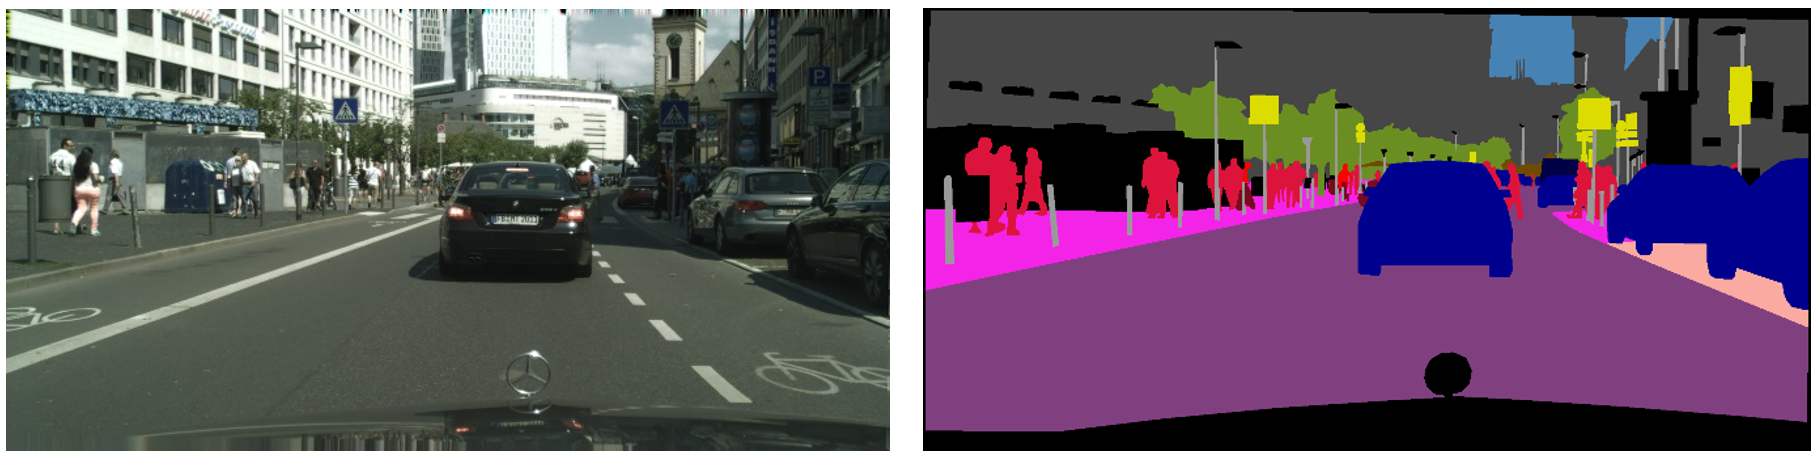
\includegraphics[width=\textwidth]{res/cityscapes-segmentation-sample.png}
    \caption{An example of an annotated semantic segmentation image from the Cityscapes dataset \cite{cordts_cityscapes_2016}.}
    \label{fig:cityscapes_segmentation_example}
\end{figure}

Segmentation is a key pre-processing task for many applications, such as self-driving cars and robotics. To safely drive, a self-driving car must be able to identify the shape, course, and edges of the road in front of it, not only identify it as a road, for instance. Medical analysis is another key segmentation task that helps automate essential biomedical tasks, such as CT or MRI image analysis \cite{hesamian_deep_2019}. Other applications include satellite mapping, video surveillance, augmented reality, damage detection, and domain transformation \cite{richter_enhancing_2021}.

Semantic segmentation is distinguished from other core computer vision tasks through its density and complexity. Density is key in segmentation as the output is pixel-wise. A significant amount of information must be known about each pixel in the image to accurately segment it, especially for the boundaries between images. The increase in computational cost is also intuitive - generating an output that has the same dimensions as the model input will always be more computationally intensive than an equivalent classification model that simply outputs a single vector. This, combined with the complexity of producing training data for the segmentation task, means there has been significant research into effectively applying semantic segmentation to a number of relevant real-world domains, with domain-specific applications often being necessary. My research has been into one of these domains - structural crack segmentation - as well as the more general concept of semantic segmentation domain adaptation, which improves the ability to use existing labelled data to apply semantic segmentation to any domain.

\section{Motivation}
Semantic segmentation is a complex problem on many levels. Models that produce densely detailed output in general require specialised architectures, whether this is through an encoder-decoder approach that uses a traditional vision model as a backbone \cite{chen_deeplab_2017} or via a wholly unique architecture \cite{yu_bisenet_2018}. Additionally, the process of producing manually labelled pixel-level data for semantic segmentation (\autoref{fig:cityscapes_segmentation_example}) is extremely expensive and time-consuming compared to other tasks. The popular Cityscapes dataset, for example, required over 1.5 hours of manual labelling for each of the 5000 finely labelled images \cite{cordts_cityscapes_2016}. Therefore, significant research has gone into the architecture and training aspect of semantic segmentation to improve its usability for real-world applications.

One aspect of research for applications is usage-specific architectures. Medical segmentation models, for example, may seek to maximise segmentation accuracy and detail without prioritising prediction speed \cite{ronneberger_u-net_2015}, whereas tasks needing real-time segmentation, such as self-driving cars, may use architectures that sacrifice some accuracy and detail but can produce many predictions per second \cite{poudel_fast-scnn_2019}. Structural crack segmentation is one such domain, where a relatively simple issue (segment only crack vs non-crack) requires fine resolution detail due to the thin nature of cracks, while also preferring efficient performance due to the large amount of data that must be processed. Therefore, one of the goals of this research was to investigate more performant efficient crack segmentation architectures.

Unsupervised domain adaptation (UDA) is a different means of applying segmentation to the real world. It involves taking the "knowledge" a segmentation model learns on one labelled dataset (e.g. The GTA5 dataset \cite{richter_playing_2016}) and applying it to an unlabelled task. While rarely as effective as using labelled data, UDA can produce acceptable results in a new domain without the extremely expensive process of manually labelling data. UDA can be exceptionally valuable for improving the accessibility of semantic segmentation by eliminating the need for labelling, combatting one of the key roadblocks to permitting individuals globally to take advantage of image segmentation. In this research, we further investigate UDA for semantic segmentation, placing specific focus on segmentation transformer architectures as the transformer has been found to be extremely effective for domain adaptation tasks \cite{yang_tvt_2021} \cite{xu_cdtrans_2021} \cite{hoyer_daformer_2022}. We also investigate ways of applying fast semantic segmentation models to domain adaption. We find this to be an under-explored area, despite being a key component of effectively and accessibly applying semantic segmentation without extensive resources, in combination with UDA. Efficient segmentation also helps combat the extensive energy usage of machine learning globally.


\section{Background}
This section includes a general review of semantic segmentation relevant to the research, with more specific background information appearing in the respective chapters.

As with most computer vision applications, deep convolutional neural networks (CNNs) traditionally achieved state-of-the-art results on semantic segmentation tasks for accuracy and efficiency. The superior performance of CNNs is often cited to be due to their possession of vision-specific inductive biases. Translational equivariance means that patterns present anywhere in an image will be extracted in the same way due to the constant convolution kernel that “slides” across the input. Locality means that CNNs, due to the limited size of each kernel, will inherently put stronger weights towards input features that are closer together in 2D space (\autoref{fig:receptive_field}) \cite{zhang_dive_2019}. All of this is achieved with fixed-size kernels, meaning the number of parameters that must be trained for any model does not increase with image size. Novel advances in general computer vision are typically first made on the simpler image classification task, then transferred to other tasks like segmentation.


\begin{figure}[t]
    \centering
    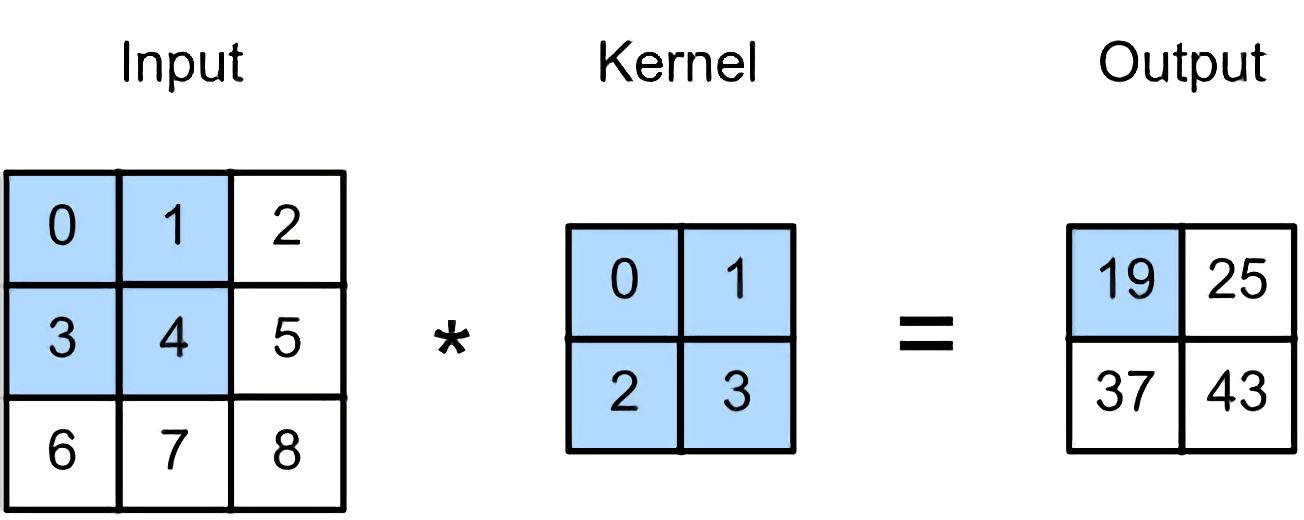
\includegraphics[scale=0.7]{res/convolution.png}
    \caption{A single step in the 2D convolution of an input tensor with a kernel \cite{zhang_dive_2019}. The next stage would be the computation of $25$ via $1 \times 0 + 2 \times 1 + 4 \times 2 + 5 \times 3$.}
    \label{fig:convolution}
\end{figure}

\begin{figure}[hb]
    \centering
    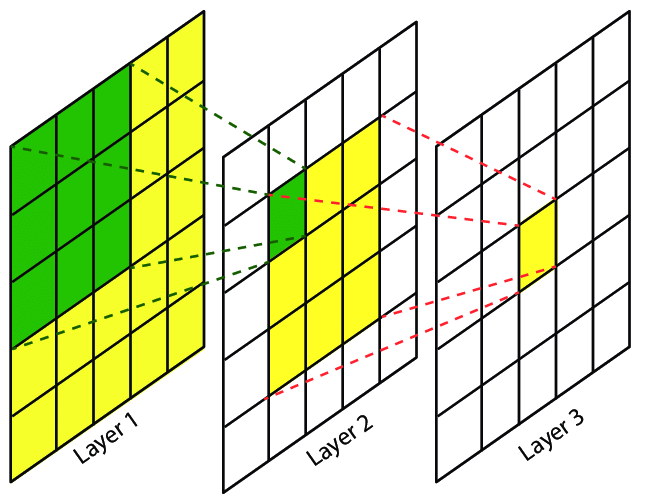
\includegraphics[scale=0.3]{res/receptive-field.png}
    \caption{A visualisation of locality across CNN layers \cite{lin_maritime_2017} - the neuron in each layer is only defined by the spatially close neurons in the previous layer. This also demonstrates CNNs' limited receptive field.}
    \label{fig:receptive_field}
\end{figure}

Most semantic segmentation approaches follow some kind of encoder-decoder structure \cite{zhang_dive_2019}. This approach consists of two parts. First, the encoder maps the input sequence to an abstract representation, typically known as a feature space. Many segmentation models, starting with FCN (Fully Convolutional Network) \cite{long_fully_2015}, use an existing classification network, called the "backbone", for this feature extraction. The decoder then reconstructs an output image from its feature representation, in this case into a segmentation map. U-Net \cite{ronneberger_u-net_2015}, ubiquitous in medical segmentation applications, is an early example of a backbone-less encoder-decoder for segmentation.

\begin{figure}[t]
    \centering
    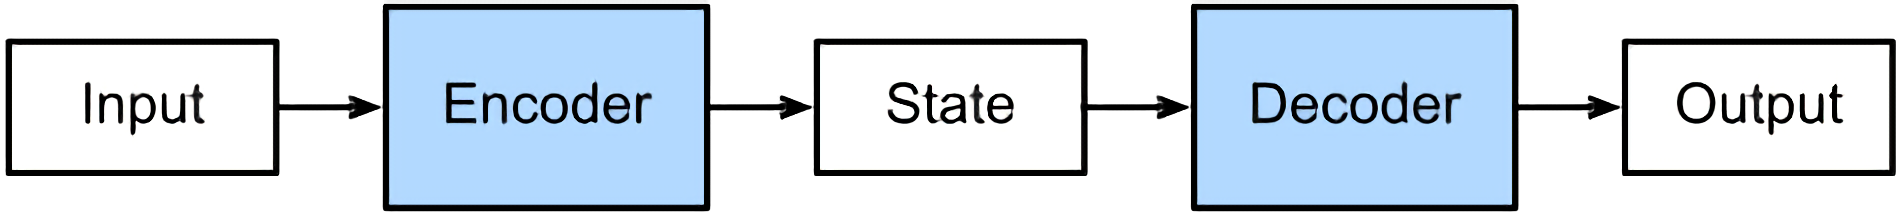
\includegraphics[width=\textwidth]{res/encoder-decoder.png}
    \caption{The encoder-decoder architecture \cite{zhang_dive_2019}.}
    \label{fig:encoder_decoder}
\end{figure}

Extraction of features at multiple scales is also important for dense prediction - a car in the distance will be differently sized to a car in the foreground, but both should be labelled accurately. This can be addressed by feeding in and parsing inputs at multiple scales, as in RefineNet \cite{lin_refinenet_2016} or using multi-scale pooling techniques, such as Spacial Pyramid Pooling (SPP) \cite{he_spatial_2014}.

\begin{figure}[h]
    \centering
    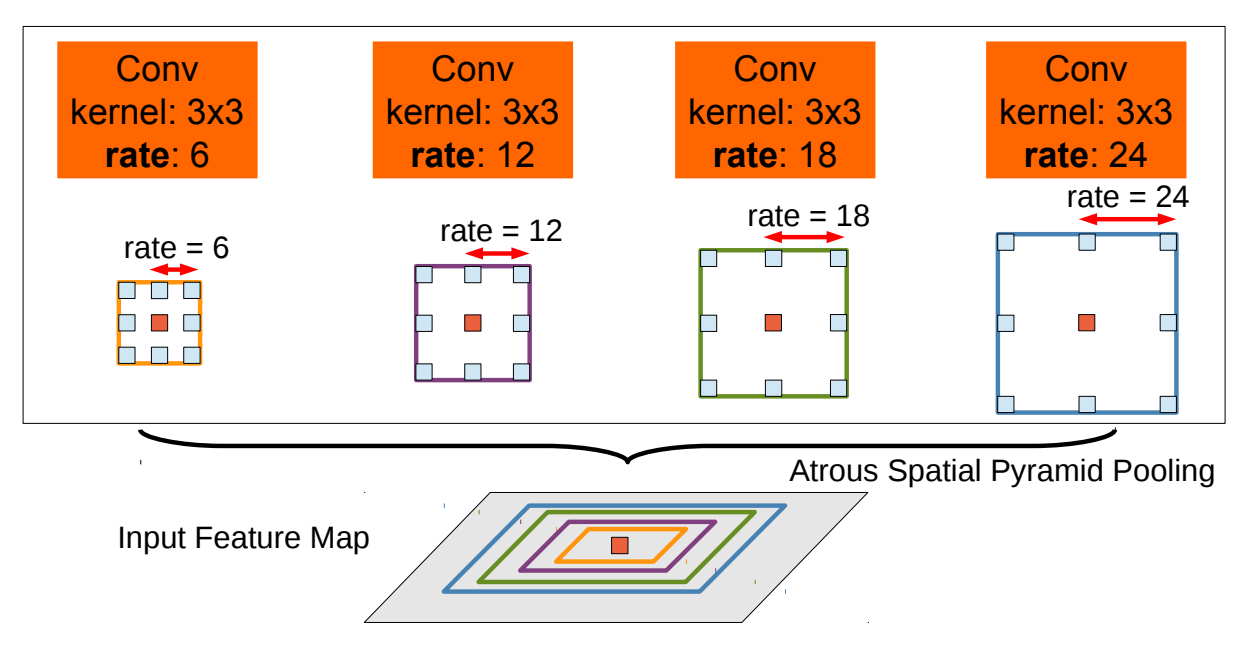
\includegraphics[scale=0.5]{res/deeplab-aspp.png}
    \caption{Visualisation of atrous spatial pyramid pooling \cite{chen_deeplab_2017}.}
    \label{fig:deeplab_aspp}
\end{figure}

Today, the DeepLab series of models is considered a benchmark for performant segmentation CNNs. DeepLab \cite{chen_semantic_2016} introduced the atrous convolution, which adds gaps between the weights used to inform the next layer’s pixels. This permits a larger receptive field without significantly increasing model parameters. DeepLabV2 \cite{chen_deeplab_2017} builds on this via Atrous Spatial Pyramid Pooling (ASPP), which combines PSPNet’s \cite{zhao_pyramid_2017} multi-scale features with a wider receptive field (\autoref{fig:deeplab_aspp}). DeeplabV3 \cite{chen_rethinking_2017} introduces a deeper architecture and adds a resizing component to ASPP that better suits atrous convolution’s large receptive field. DeepLabV3+ \cite{chen_encoder-decoder_2018} introduced an encoder-decoder design with DeepLabV3 as the encoder, and applies a simple decoder to better refine class boundaries. DeeplabV3+ achieves 82.1\% mIoU on the Cityscapes dataset \cite{cordts_cityscapes_2016}, a common benchmark for segmentation models.

% ------------------------------------------------------------------------------
% Crack Segmentation
% ------------------------------------------------------------------------------
\chapter{Crack Segmentation}
Crack segmentation is an example of a highly specialised semantic segmentation task with specific requirements. In this chapter, we explore novel architectures optimised to perform crack segmentation efficiently and at high-resolution.

\section{Background}
% \subsection{Semantic Segmentation}
\subsection{Crack detection and segmentation}
Crack detection has been a growing research area in recent years \cite{hamishebahar_comprehensive_2022}. The detection of surface-level cracks is significant in evaluating the health of structures, and achievable using automated camera-based approaches with modern computer vision techniques. Zhang \textit{et al.} \cite{zhang_road_2016}, for instance, proposed an early CNN for performing crack detection on a dataset of 500 crack images. While approaches initially focused on object detection and classification, many recent studies apply semantic segmentation \cite{hamishebahar_comprehensive_2022} due to the valuable additional information on crack shape and size it provides. Initial approaches often applied existing segmentation networks or backbones to crack detection, such as U-Net \cite{david_jenkins_deep_2018} and SegNet \cite{chen_pavement_2020}.

There are two unique issues in crack segmentation compared to other segmentation tasks. First, the thin and fine-grained nature of cracks means especially dense features must be maintained throughout the model, as any reduction in feature resolution will cause major inaccuracies in fine crack shapes. Secondly, cracks typically make up a minority of a given input image even when they are present ($<5\%$ of pixels), resulting in class imbalance. DeepCrack \cite{liu_deepcrack_2019} computes multi-scale features to ensure large and thin cracks are accurately segmented and applies a multi-head class-balanced loss to address class imbalance. FPHBN \cite{yang_feature_2019} instead derives multi-scale information via a feature pyramid. MR-CrackNet \cite{nayyeri_multi-resolution_2021} applies a modified ResNet \cite{he_deep_2015} backbone, addressing the maintaining of feature resolution by upsampling extracted features after each block.
Many of the above approaches are evaluated on unique datasets not publicly available, making comparisons challenging. A number of public datasets have been proposed for crack segmentation, including CrackBgData \cite{nayyeri_multi-resolution_2021}, CRACK500 \cite{yang_feature_2019}, and others \cite{eisenbach_how_2017} \cite{shi_automatic_2016} \cite{amhaz_automatic_2016} \cite{zou_cracktree_2012}.

\begin{figure}
    \centering
    \begin{subfigure}{.5\textwidth}
        \centering
        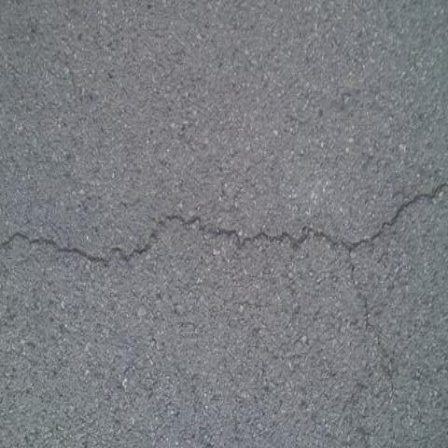
\includegraphics[width=0.8\linewidth]{res/dataset_CFD_029.png}
        \caption{Original crack image}
        \label{fig:crack-percentages-sub1}
    \end{subfigure}%
    \begin{subfigure}{.5\textwidth}
        \centering
        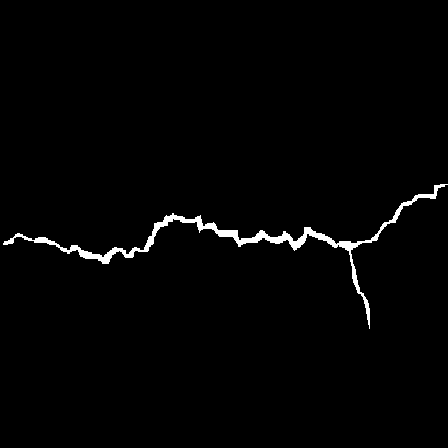
\includegraphics[width=0.8\linewidth]{res/dataset_CFD_029_label.png}
        \caption{Crack label}
        \label{fig:crack-percentages-sub2}
    \end{subfigure}
    \caption{Crack image and corresponding segmentation mask from the CFD dataset \cite{shi_automatic_2016}. Note the white `crack' class only makes up $\sim 1.5\%$ of pixels in the mask.}
    \label{fig:crack-percentages}
\end{figure}

\subsection{Fast semantic segmentation}
The density and number of predictions (typically one per input pixel) required for semantic segmentation makes it one of the most computationally expensive computer vision tasks. The large number of predictions in the output layer is itself computationally expensive, but dense predictions also typically require a higher-resolution feature map, further increasing memory and compute requirements. Many state-of-the-art segmentation models are therefore only capable of running at a speed of 2-3 predictions a second on modern hardware \cite{zhao_icnet_2018}. Since many uses of segmentation, such as self-driving cars and robotics, require  real-time inference, extensive research has been done to improve the efficiency of semantic segmentation.

ENet (Efficient Net) \cite{paszke_enet_2016} was one of the first models to explore low-resource segmentation, focusing on reasonable accuracy capable of running in real-time on mobile devices. It achieves this by making select sacrifices to minimise model parameters and computations while mitigating drops in accuracy. Input features are quickly downsampled to a low resolution ($\frac{1}{8}$th input) with few features. The model minimises the size of the decoder, and employs atrous and factorised convolutions to increase receptive field without increasing computation. E-Net achieves 58.3\% mIoU on the Cityscapes test set with 0.37M parameters, compared to the then state-of-the art DeepLab’s 63.1\% mIoU with 134.3M parameters.

Initial fast segmentation approaches had an inherent trade-off: reduced input size increases speed, as less convolutions must be performed, but reduces segmentation accuracy, as there are less fine details. ICNet \cite{zhao_icnet_2018} addresses this by taking in the same input image at different scales. High-resolution inputs are parsed through low-filter-count layers that are lightweight but still capable of extracting low-level details like edge and texture. Low-resolution inputs are parsed through more expensive high-filter-count layers capable of extracting high-level object information (e.g. “these pixels represent a car”), where the low resolution keeps computation time low. The computed features are then fused together through multiple “cascades” to produce the final features. This approach - delegating high-resolution branches to low-level details and vice versa - has become a staple of fast segmentation. BiSeNet \cite{yu_bisenet_2018} extends ICNet’s multi-resolution approach, finding that two ‘branches’, one high-resolution (the “spatial path”) and one low resolution (the “context path”) is most effective.

Many efficient segmentation models rely on innovations from other computer vision domains. The MobileNet \cite{howard_mobilenets_2017} classification models introduced the depthwise separable convolution block, which splits a standard convolution into a (far less expensive) combination of pointwise and depthwise convolution with minimal accuracy loss. MobileNetV2 \cite{sandler_mobilenetv2_2019} introduces the bottleneck residual block, which performs efficient convolutions by transforming inputs into a high-dimensional manifold. ContextNet \cite{poudel_contextnet_2018} uses a two-branch architecture like BiSeNet \cite{yu_bisenet_2018}, and introduces depthwise separable convolutions and bottleneck residual blocks for the high (shallow) and low (deep) resolution branches respectively. ContextNet’s successor, Fast-SCNN \cite{poudel_fast-scnn_2019}, has become a benchmark for fast segmentation performance. It replaces the high-resolution branch with a simple series of convolutions and skip connection for improved efficiency (\autoref{fig:fastscnn_architecture}).

\begin{figure}[h]
    \centering
    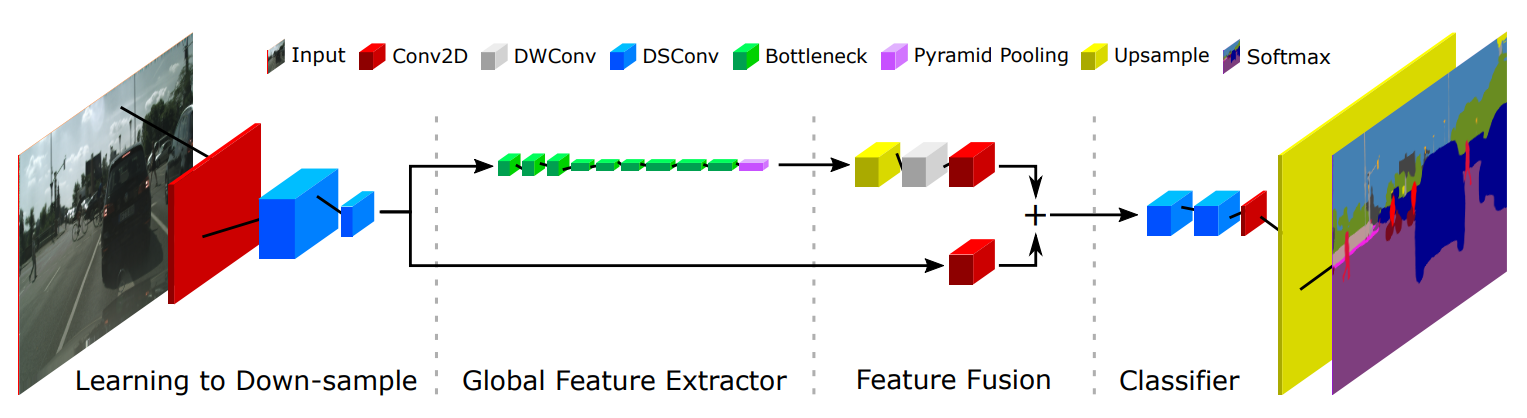
\includegraphics[width=\textwidth]{res/fastscnn-architecture.png}
    \caption{Fast-SCNN architecture \cite{poudel_fast-scnn_2019}.}
    \label{fig:fastscnn_architecture}
\end{figure}

\subsection{Efficient crack segmentation}
Processing efficiency is important when performing infrastructure crack detection due the large amount of images that must be processed when applied at scale. Various studies \cite{kerle_uav-based_2020} \cite{kang_autonomous_2018} have investigated the use of UAVs (Unmanned Aerial Vehicles) for high-speed crack segmentation, a system only viable with a highly efficient neural network such as Faster R-CNN \cite{ali_real-time_2021}. Recent studies have investigated efficient crack detection. SDDNet \cite{choi_sddnet_2019} maintains high-resolution features using a simple skip connection, and utilises depthwise separable convolutions and modified atrous spatial pyramid pooling techniques as introduced in the MobileNets \cite{howard_mobilenets_2017} and DeepLabV3+ \cite{chen_rethinking_2017} respectively. STRNet \cite{kang_efficient_2021} applies multi-head attention to the crack detection task, as well as a squeeze and excitation method for maintaining high feature detail.
These approaches are similar to traditional efficient segmentation architectures in the maintaining of different architectural components focusing on low and high-level features, but typically with a particular focus on high-resolution feature maps for the fine-grained crack segmentation task.

\section{The SC-CrackSeg model}

The use of a separate branch for maintaining high-resolution features in crack segmentation models \cite{nayyeri_multi-resolution_2021} is similar to the deep-brach/shallow-branch approach used in efficient segmentation models \cite{yu_bisenet_2018} \cite{poudel_contextnet_2018}. This key realisation lead to the development of our model, SC-CrackSeg, which sought to apply a proven architectural paradigm to achieve lightweight, efficient, and performant crack segmentation. We used our team's previous model, SCMNet \cite{singha_scmnet_2021}, as a baseline. In SCMNet, deep (low-resolution) and shallow (high-resolution) features are repeatedly merged and feature-extracted before being fed back into their respective branches, maintaining both global and local features while permitting both to learn from one another. We posit applying this approach to crack segmentation would allow for the efficient learning of global and high-resolution crack features while retaining the computational efficiency such approaches often struggle to achieve.

\begin{figure}[h]
    \centering
    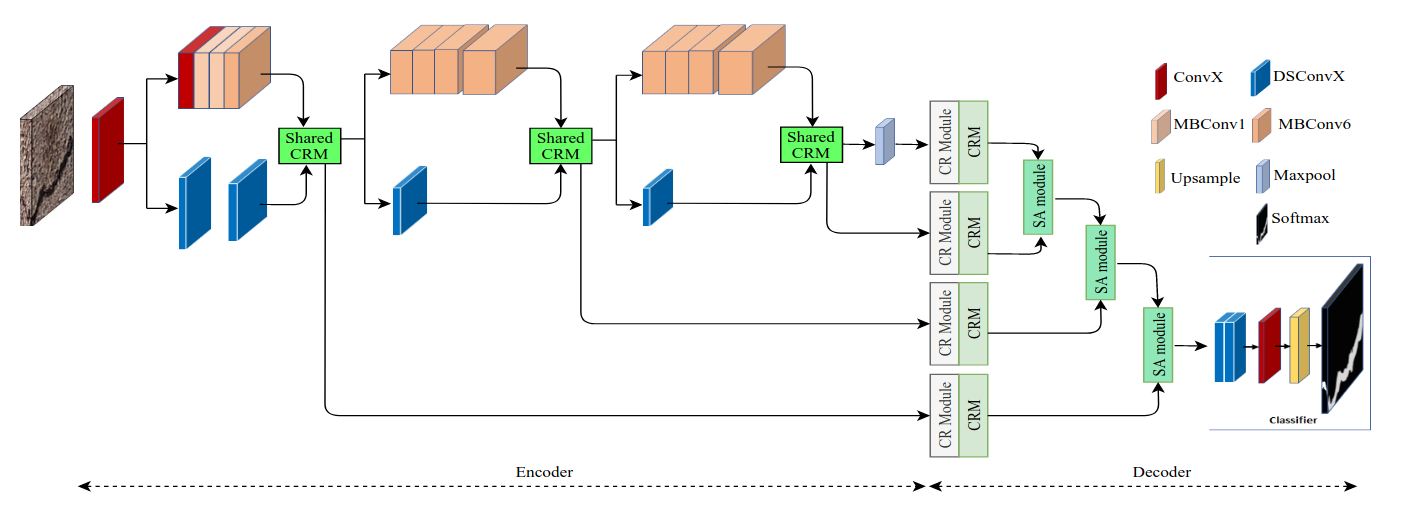
\includegraphics[width=0.75\textwidth]{res/sc-crackseg-architecture.png}
    \caption{Architecture of SC-CrackSeg \cite{singha_sc-crackseg_2022}.}
    \label{fig:sc-crackseg-architecture}
\end{figure}

We make a number of changes to SCMNet to better suit it to the crack segmentation task and generally improve it. We move from a two-input model to a single-input model to improve efficiency and simplicity of implementation. We modify SCMNet's Context Mining Module (CMM) by eliminating its image pooling components which contribute to boundary degeneration - especially significant with crack segmentation's fine boundaries. We also deploy a simplified feature fusion module, inspired by BiSeNet \cite{yu_bisenet_2018}, to aggregate the final features extracted from the two branches.

\subsection{Datasets}
Another key innovation was the use of a unified dataset to evaluate SC-CrackSeg's performance. As many datasets used to train and evaluate other crack segmentation models are either small or not publicly available, we use a combined dataset of 12 different source crack segmentation datasets, all using the same labelling scheme. Retrieved from Kaggle \footnote{\url{https://www.kaggle.com/datasets/lakshaymiddha/crack-segmentation-dataset}}, this dataset provided us with 9505 train and 1695 test images. While unorthodox, we find this dataset to be exceptionally challenging due to the large variety of image types it contains, from extremely thick to extremely thin cracks, different surfaces, and even samples that contain no cracks (which can be considered testing for false positives). We identify and amend a number of issues in this dataset, and then use it to benchmark a number of existing state-of-the art crack segmentation approaches against SC-CrackSeg.

\subsection{Class imbalance}
Besides feature resolution, class imbalance is the other key domain-specific issue in crack segmentation \cite{hamishebahar_comprehensive_2022}. Due to the overwhelming majority of "no crack" classes, the model is implicitly encouraged to prioritise predicting them in each pixel. Therefore, models must often be encouraged to accurately predict the minority class through class balancing. This is most commonly done by simply weighting the produced model losses depending on the sample, with less common samples receiving higher weights. In semantic segmentation, where each pixel in an image effectively contains its own loss, we achieved this by using the ground truth to map a multiplication operation onto the per-pixel losses. The weights chosen for each class can vary, but the inverse of each class proportion in the training dataset is typically used \cite{kochkarev_data_2020}.

\pagebreak

% \hspace*{4mm}
\begin{lstlisting}[language=Python, caption=Weighted categorical crossentropy function in python using TensorFlow 2.1]
def weighted_cat_crossentropy(target, output, class_weights, axis=-1):
    # scale preds so that the class probas of each sample sum to 1
    output = output / math_ops.reduce_sum(output, axis, True)

    epsilon_ = _constant_to_tensor(epsilon(), output.dtype.base_dtype)
    output = clip_ops.clip_by_value(output, epsilon_, 1. - epsilon_)

    # compute per-pixel categorical losses
    cat_losses = tf.reduce_sum(target * math_ops.log(output), axis=axis)
    
    # Apply class weights
    weight_indices = tf.argmax(target, axis=-1)
    weight_map = tf.gather(class_weights, indices=weight_indices)
    weighted_cat_losses = cat_losses * weight_map
    
    return - 1. * weighted_cat_losses
\end{lstlisting}

\subsection{Initial Results}
We find SC-CrackSeg's combination of efficiency and performance to be highly competitive. Typically, mean intersection over union (mIoU) is used to present segmentation results, but crack segmentation is highly unbalanced - the size of one class (no crack) would skew model results. Therefore, we also assess using F1 score to better consider false positives and false negatives across classes. In terms of pure performance, SC-CrackSeg is slightly beaten by other models like DeepCrack (\autoref{tab:sc-crackseg-initial-performance-comparison}). DeepCrack achieves 77.23\% mIoU and 85.49\% mean F1 score, while SC-CrackSeg produces 77.0477\% mIoU and 85.34\% mean F1. However, SC-CrackSeg is far more efficient (\autoref{tab:sc-crackseg-initial-efficiency-comparison}), over 12 times smaller and 4 times faster than DeepCrack. DeepCrack possesses 14.7 million parameters (size of weights) and requires 78.8GFlops of computation per prediction, while SC-CrackSeg requires only 1.24 million parameters and 2.8 GFLOPs. When optimised for performance using Nvidia's TensorRT, SC-CrackSeg achieves a speed of 220 predictions per second.


\begin{table*}[ht]
    \begin{adjustbox}{width=\columnwidth,center}
        % \centering
        \begin{tabular}{|c|c|c|c|c|c|c|c|c|c|c|c|c|c|}
            \hline
                                                              &                & \multicolumn{3}{|c|}{\textbf{IoU}} & \multicolumn{3}{|c|}{\textbf{F1 score}} & \multicolumn{3}{|c|}{\textbf{Precision}} & \multicolumn{3}{|c|}{\textbf{Recall}}                                                                                                      \\
            \hline
            {Model}                               u           & {Accuracy}     & {BG}                               & {Crack}                                 & {mIoU}                                   & {BG}                                  & {Crack} & {mF1}          & {BG}    & {Crack} & {aP}           & {BG}    & {Crack} & {aR}           \\
            \hline
            {DeepLab \cite{chen_encoder-decoder_2018}}        & {98.43}        & {98.50}                            & {52.28}                                 & {75.39}                                  & {99.24}                               & {68.66} & {83.95}        & {98.97} & {79.25} & {89.11}        & {99.52} & {60.57} & {80.05}        \\
            \hline
            {U-Net \cite{}}                                   & {98.18}        & {98.2}                             & {48.97}                                 & {73.58}                                  & {99.09}                               & {65.74} & {82.42}        & {98.96} & {70.62} & {84.79}        & {99.23} & {61.49} & {80.20}        \\
            \hline
            {SegNet\cite{chen_pavement_2020}}                 & {98.27}        & {98.30}                            & {52.17}                                 & {75.23}                                  & {99.14}                               & {68.57} & {83.85}        & {99.09} & {71.15} & {85.12}        & {99.19} & {66.17} & {82.63}        \\
            \hline
            {DeepCrack\cite{liu_deepcrack_2019}}              & \textbf{98.52} & {98.57}                            & {55.89}                                 & \textbf{77.23}                           & {99.28}                               & {71.70} & \textbf{85.49} & {99.13} & {77.95} & {84.54}        & {99.44} & {66.38} & \textbf{82.91} \\
            \hline
            {MR-CrackNet\cite{nayyeri_multi-resolution_2021}} & {97.88}        & {97.19}                            & {47.69}                                 & {72.80}                                  & {98.95}                               & {64.58} & {81.76}        & {99.11} & {62.59} & {80.85}        & {98.79} & {66.71} & {82.70}        \\
            \hline
            {SCMNet\cite{singha_scmnet_2021}}                 & {98.39}        & {98.41}                            & {51.33}                                 & {74.87}                                  & {99.20}                               & {67.84} & {83.52}        & {98.91} & {77.51} & {88.21}        & {99.48} & {60.32} & {79.30}        \\
            \hline
            {SC-CrackSeg}                                     & \textbf{98.52} & {98.52}                            & {55.55}                                 & {77.04}                                  & {99.25}                               & {71.43} & {85.34}        & {99.05} & {78.14} & \textbf{88.59} & {99.46} & {65.78} & {82.32}        \\
            \hline
            \multicolumn{11}{l}{}
        \end{tabular}
    \end{adjustbox}
    \caption{Performance evaluation of different models on crack test set}%\label{tab5}
    \label{tab:sc-crackseg-initial-performance-comparison}
\end{table*}

\begin{table*}
    \begin{adjustbox}{width=\columnwidth,center}
        \centering
        \begin{tabular}{|c|c|c|c|c|c|c|c|c|c|}
            \hline
            {}            & {}           & {}           & \multicolumn{5}{|c|}{\textbf{FPS of different types of model}} & {}          & {}                                                                                                                    \\
            \hline
            {Model}       & {Param.(M)}  & {GFLOPs}     & {Keras}                                                        & {TF}        & {TF-TRT32}   & {TF-TRT16}   & {TRT-INT8}   & {\begin{tabular}{@{}c@{}}Training\\time(s)\end{tabular}} &
            {\begin{tabular}{@{}c@{}}Model \\size (MB)\end{tabular}}                                                                                                                                                                                           \\
            \hline
            {DeepLab}     & {41.0}       & {78.8}       & {20}                                                           & {21}        & {32}         & {48}         & {82}         & {415}                                                    & {158}         \\
            \hline
            {U-Net}       & {31.0}       & {1740.0}     & {31}                                                           & {30}        & {39}         & {39}         & {50}         & {348}                                                    & {355}         \\
            \hline
            {SegNet}      & {29.4}       & {245.0}      & {32}                                                           & {32}        & {44}         & {45}         & {56}         & {316}                                                    & {225}         \\
            \hline
            {DeepCrack}   & {14.7}       & {123.0}      & {33}                                                           & {33}        & {48}         & {50}         & {65}         & {257}                                                    & {112}         \\
            \hline
            {MR-CrackNet} & {17.7}       & {331}        & {14}                                                           & {14}        & {25}         & {28}         & {45}         & {1013}                                                   & {203}         \\
            %\hline
            %{MR-CrackNet} & {17.7} & {331} & {} &  {} & {} & {} &  {} & {} & {}\\
            \hline
            {SCMNet}      & \textbf{1.2} & {3.3}        & {61}                                                           & {67}        & {111}        & {111}        & {114}        & {182}                                                    & {10.7}        \\
            \hline
            {SC-CrackSeg} & {1.24}       & \textbf{2.8} & \textbf{70}                                                    & \textbf{78} & \textbf{216} & \textbf{216} & \textbf{220} & \textbf{93}                                              & \textbf{10.8} \\
            \hline
            \multicolumn{10}{l}{}
        \end{tabular}
    \end{adjustbox}
    \caption{Efficiency analysis against SC-CrackSeg}
    \label{tab:sc-crackseg-initial-efficiency-comparison}
\end{table*}


\section{Further exploration of SC-CrackSeg and Competitors}
\subsection{The Performance of SDDNet}
While our team implemented a number of existing crack segmentation models for fair comparison against SC-CrackSeg, some could not be completed due to time limitations. Notably, a from-scratch implementation of 2019's SDDNet \cite{choi_sddnet_2019} was in development, but could not be completed in time for the publication. The SDDNet implementation has since been completed and evaluated, and results are surprising: SDDNet, at a similar parameter count and computational efficiency, outperforms all other models tested by a significant margin.

SDDNet was introduced in 2019 as a novel design specifically targeting the low class count and large object shapes present in the crack segmentation task while focusing on efficiency. A single-branch encoder-decoder model, SDDNet uses atrous spacial pyramid pooling and dense skip connections to extract features. Notably, it performs all of its depthwise separable convolutions in reverse, doing pointwise convolution first to initially reduce dimensionality and further reduce computation over the traditional method. While not explicitly stated, we intuit that the reduced channel resolution from performing depthwise first is not as significant in a low-class task like crack segmentation, where the feature space is relatively semantically sparse. It also removes the global average pooling component of its Atrous Spacial Pyramid Module as it was found to strongly regularise, detrimental to a low-parameter model.

\begin{figure}[ht!]
    \centering
    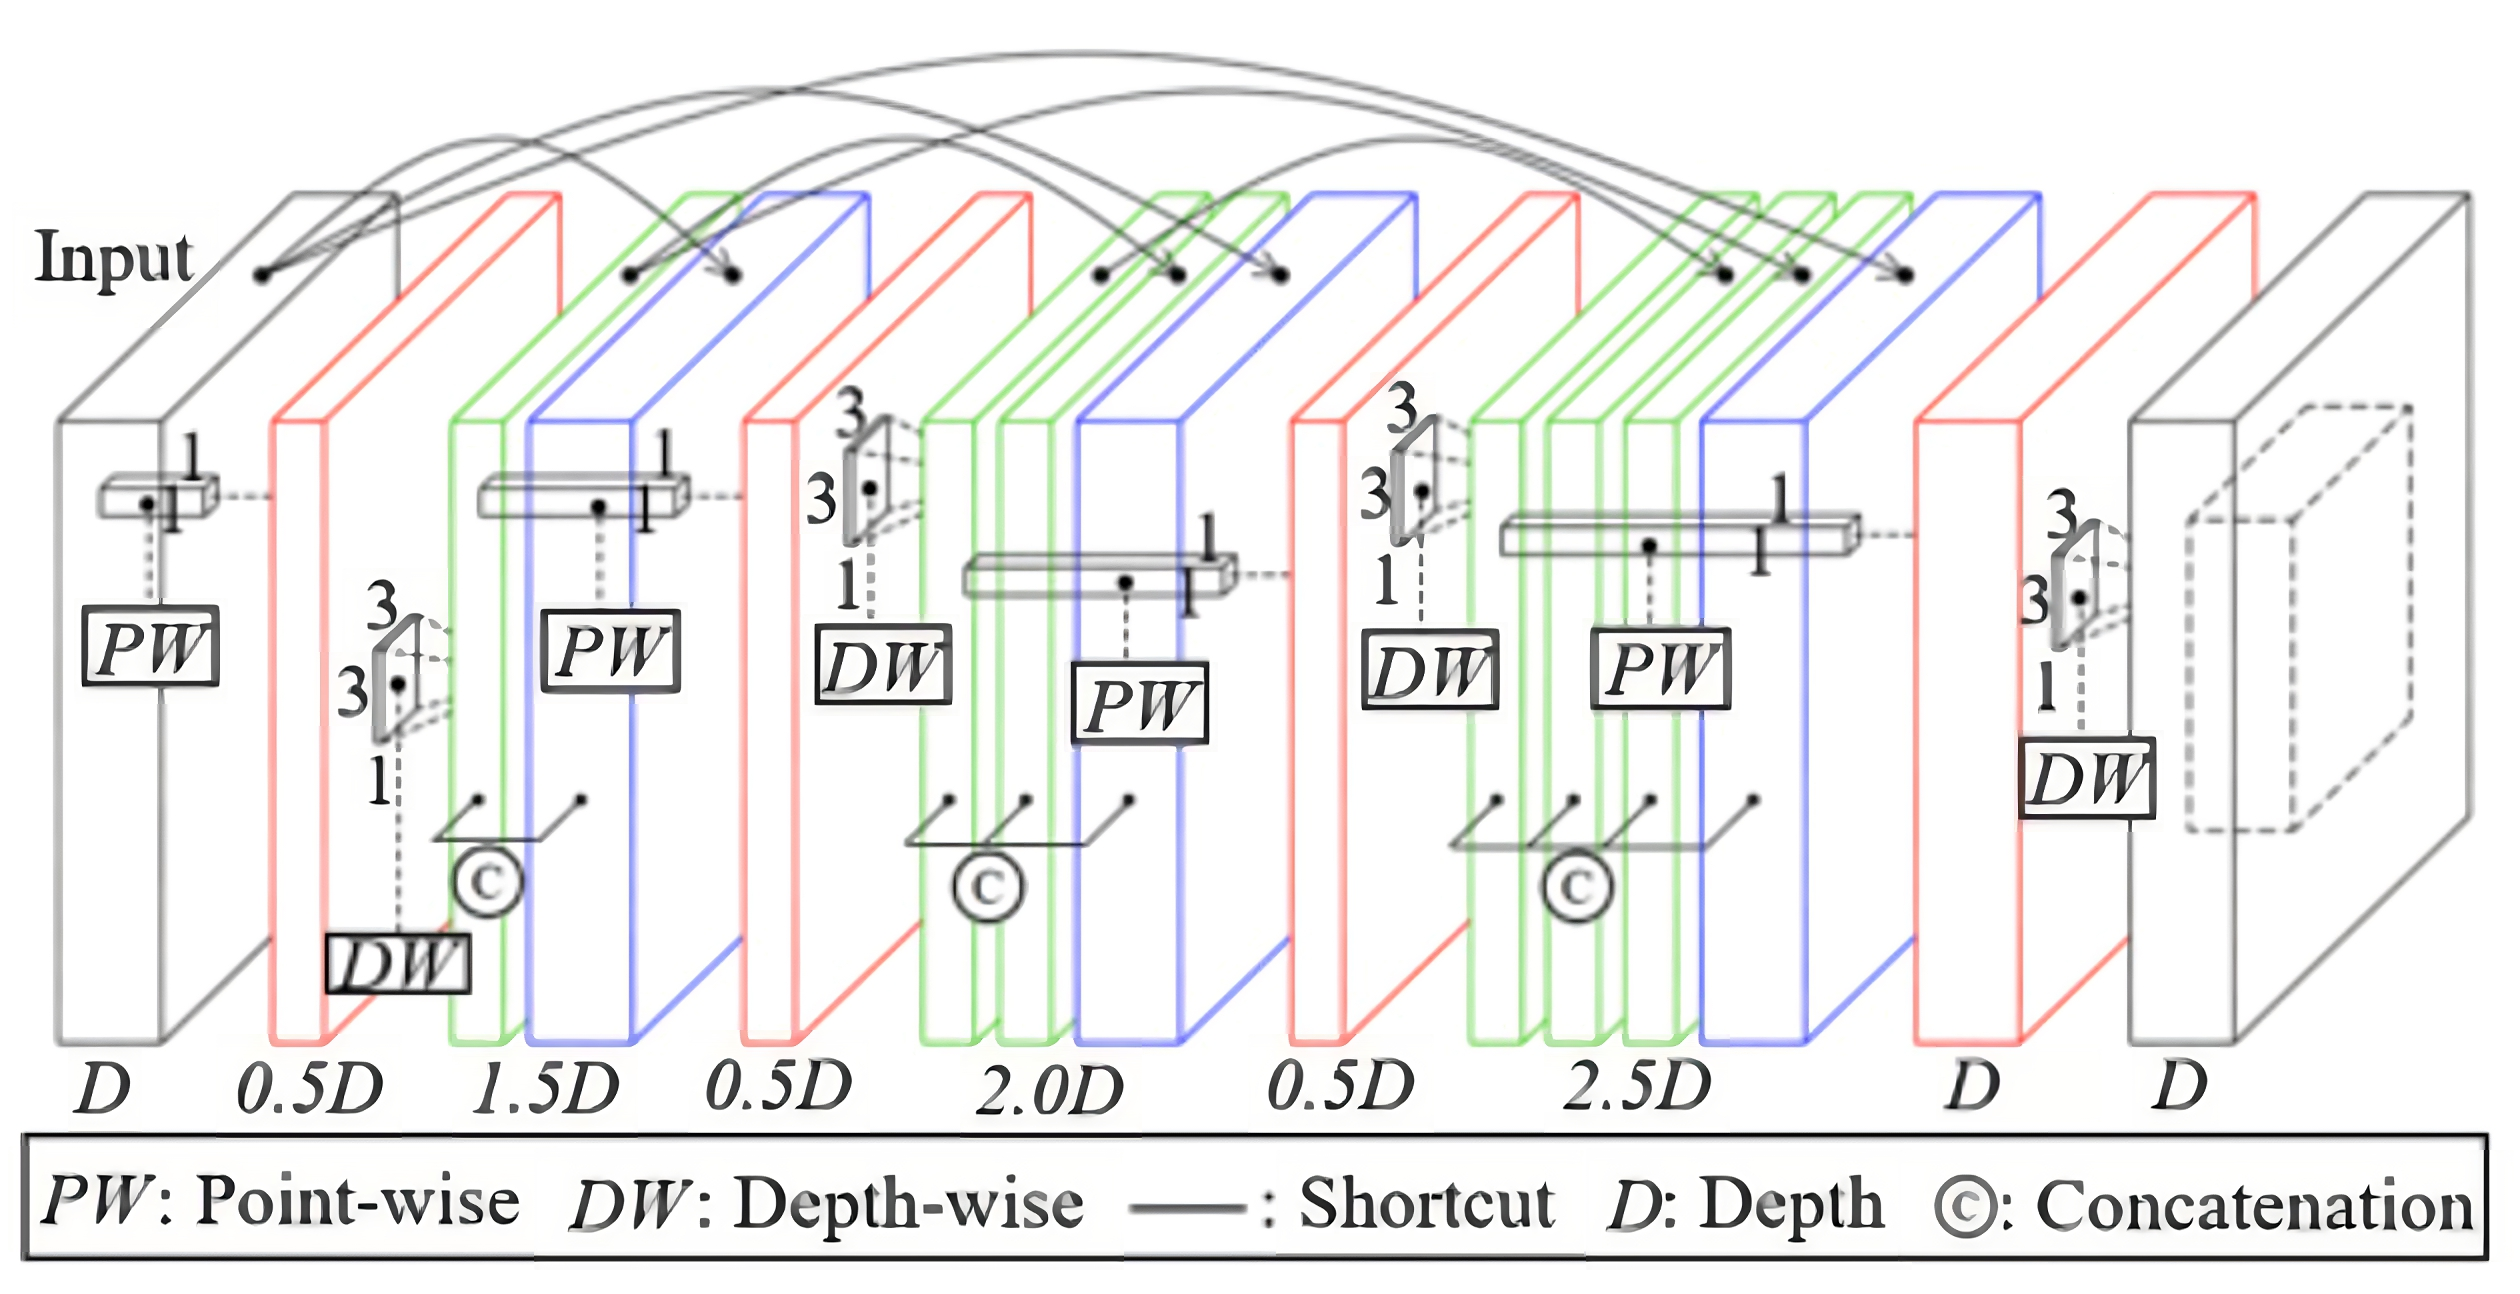
\includegraphics[width=0.5\textwidth]{res/sddnet-densep-module.png}
    \caption{SDDNet's \cite{choi_sddnet_2019} DenSep module. The number of channels maintained throughout the module is constant, though depth is periodically increased through concatenation and skip connections.}
    \label{fig:densep-module}
\end{figure}

SDDNet is primarily made up of DenSep modules, which consist of repeated reverse DSConv operations. The output of each operation is then fed into the input of all subsequent ones, permitting a large amount of feature extraction while keeping the number of channels very low, and thus computation extremely efficient. The authors found that, in terms of multiplications done, the DenSep module reduces computing cost by over 70\% an approach using traditional convolutions.

Finally, SDDNet's decoder upsamples input features in two stages, applying a skip connection from early in the model (when features were high resolution) combined with separable convolutions between the upsamples. This aids in the refinement of feature boundaries before they are upsampled further. SCMNet identified that multi-stage upsampling was, while more computationally expensive, significantly more effective than a single upsample \cite{singha_scmnet_2021}. SC-CrackSeg uses a similar approach to SDDNet, upsampling multiple times using skip connections from previous positions in the model. However, SC-CrackSeg downsamples far more than SDDNet, and only performs skip connections during the lower-resolution stages of upsampling.

\subsection{Modifications to CrackSeg}

\begin{figure*}[]
    \centering
    \begin{subfigure}[b]{0.3\textwidth}
        \centering
        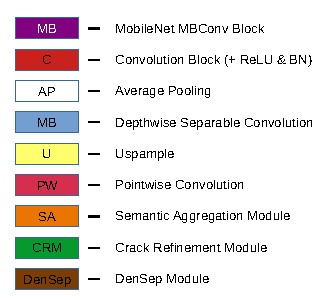
\includegraphics[width=\textwidth]{res/crack-experiment-diagrams/legend.pdf}
        \label{fig:sc-crackseg-versions-legend}
    \end{subfigure}
    \begin{subfigure}[b]{0.6964\textwidth}
        \centering
        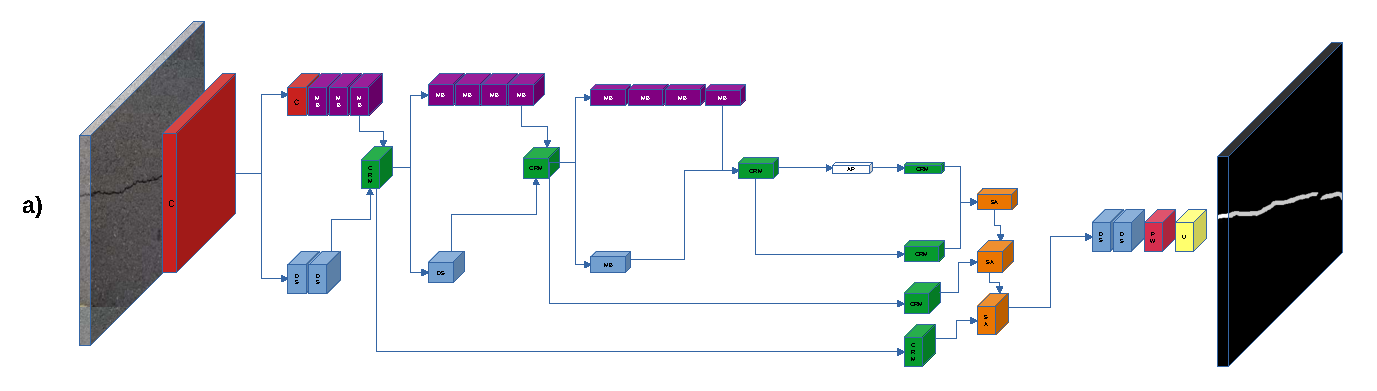
\includegraphics[width=\textwidth]{res/crack-experiment-diagrams/sc-crackseg.pdf}
        \caption{SC-CrackSeg}
        \label{fig:sc-crackseg-versions-sc-crackseg}
    \end{subfigure}
    \begin{subfigure}[b]{0.6964\textwidth}
        \centering
        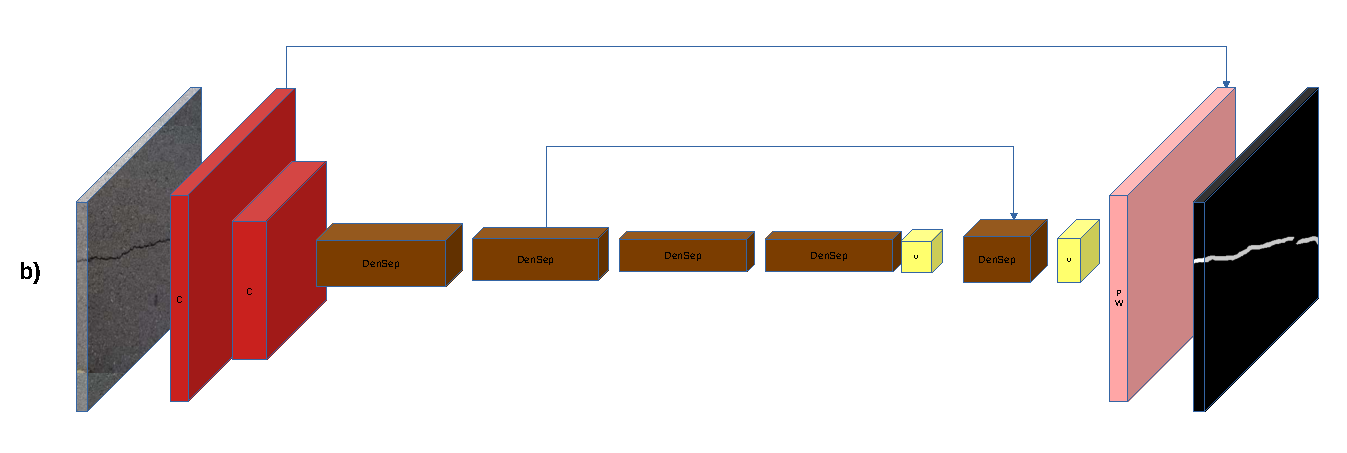
\includegraphics[width=\textwidth]{res/crack-experiment-diagrams/sddnet.pdf}
        \caption{SDDNet}
        \label{fig:sc-crackseg-versions-sddnet}
    \end{subfigure}
    \begin{subfigure}[b]{0.6964\textwidth}
        \centering
        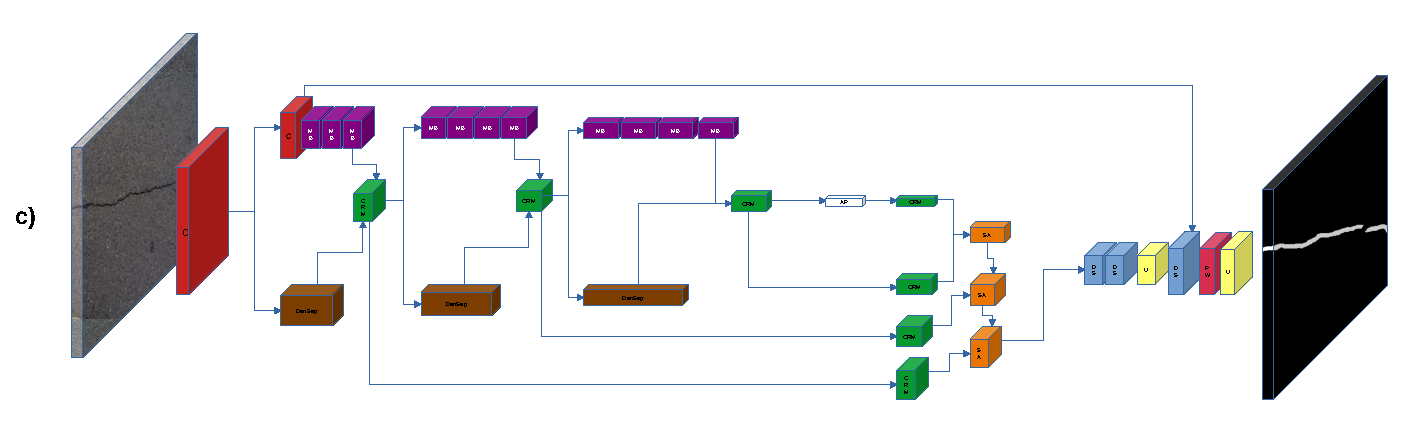
\includegraphics[width=\textwidth]{res/crack-experiment-diagrams/sc-crackseg-densep-skip.pdf}
        \caption{SC-CrackSeg with DenSep and skip connection}
        \label{fig:sc-crackseg-versions-sc-crackseg-densep-skip}
    \end{subfigure}
    \begin{subfigure}[b]{0.6964\textwidth}
        \centering
        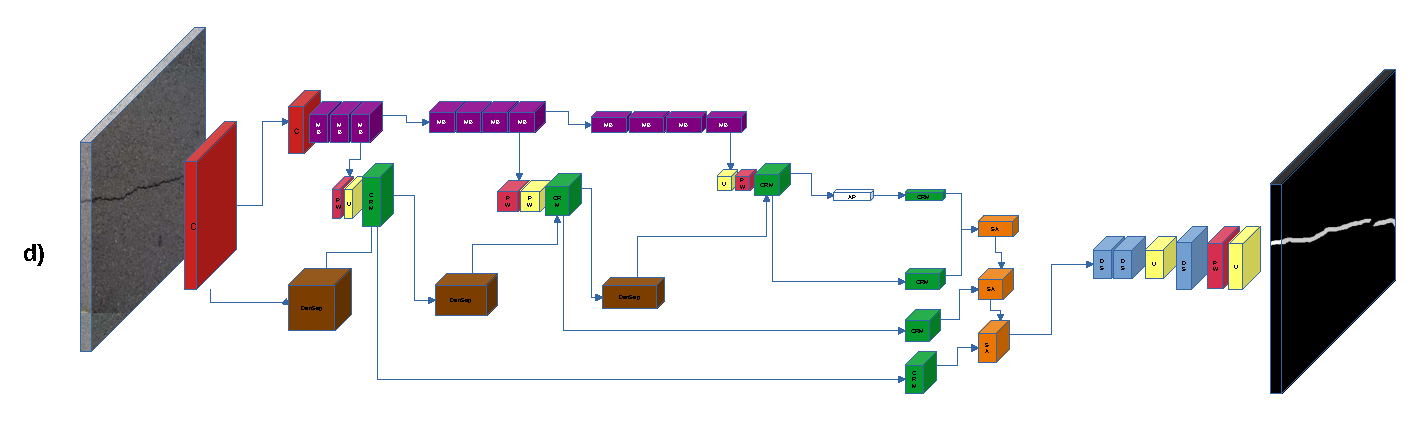
\includegraphics[width=\textwidth]{res/crack-experiment-diagrams/sc-crackseg-densep-upsample.pdf}
        \caption{SC-CrackSeg with DenSep and upsampled shallow branch}
        \label{fig:sc-crackseg-versions-sc-crackseg-densep-upsample}
    \end{subfigure}

    \caption{Diagrams representing significant architectures during experimentation.}
    \label{fig:sc-crackseg-versions}
\end{figure*}

Based on the strong performance of a simple model like SDDNet, we hypothesised that SC-CrackSeg could be optimised further towards the crack segmentation task. Therefore, we experimented with our architecture, seeking to take into consideration many of the design choices made in successful models like SDDNet.

We begin model development with a naive intuition: SC-CrackSeg's issues were caused by a lack of direct adaptation to the crack segmentation scenario - the model was too deep and too low-resolution. Two things have been identified throughout the review of crack segmentation - output quality depends on high-resolution, and the actual act of class distinguishing is simple relative to other tasks. The intuition was that decreasing the amount of downsampling done by the model would improve the granularity of produced features, while reducing the number of channels would counteract the performance cost of this operation while only minimally affecting results due to the simple semantic space. However, experiments showed the problem was not that simple. Increasing resolution immediately became prohibitively expensive in terms of performance, while decreasing channels significantly (to a maximum of 64) destroyed model performance.

Upon these initial failures, we instead explored a more nuanced approach. We designed iterations of SC-CrackSeg that place focus on the shallow branch while minimising the effect on the deep branch wherever possible. Unfortunately, we found any approach increasing shallow network convolution resolution to be unfeasible when combined with the deep branch, and also found simply increasing the number of convolutions in the shallow branch had minimal effect on model performance.

Inspired by SDDNet, we replace all shallow branch blocks with DenSep modules (\autoref{fig:sc-crackseg-versions-sc-crackseg-densep-skip}). This concatenation-based approach to feature extraction allows feature resolution to be maintained in the deep branch (where it is most essential) while minimising the downsampling done, as DenSep modules only downsample in their final block (\autoref{fig:densep-module}). An initial model with only these changes achieved promising results. An issue, however, is that since the deep and shallow branches share information, their dimensions must periodically match at the 3 information sharing points in the model, forcing the shallow branch to be downsampled further than in SDDNet. This is likely to reduce output granularity. We first addressed this by adjusting the information sharing system. Information would only be shared from the deep to the shallow branch, and the shallow branch would downsample less and possess fewer channels to counteract computing costs. Information sharing could then occur by reducing the deep branch's channels via pointwise convolution and then upsampling. These combined results produced one of our final architectures (\autoref{fig:sc-crackseg-versions-sc-crackseg-densep-upsample}).

Another consideration was the significance of the gradual upsampling skip connection in SDDNet. While SC-CrackSeg already possesses a number of skip-like connections and gradual upsampling, these largely occur to at lower resolutions, and are still followed by an $8 \times$ upsample. Therefore, we added another skip connection with the early parts of the model before final output is computed. The skip connection features were initially resolved with the decoder features using another SA module as with the other skip connections in the model, but we found this to degrade performance (perhaps as the SA module failed to produce fine output at the highest resolutions). Replacing the SA module with a simple depthwise separable convolution resolved these issues. This approach was most successful, and while multiple variations were assessed, any increase in complexity (introducing upsamples or adding further skip connections) seemed to decrease model stability and quickly cause overfitting issues.

Even though our best approaches introduced SDDNet's DenSep module, we notably did not borrow another core feature - the final ASPP stage. This is as SC-CrackSeg already possesses high-quality global context refinement via its deep branch, which aggregates global context through repeated downsampling and then merges these with the more fine features.

\subsection{Experimental Setup}
All new experiments were run using my available experimental environment, which consisted of a single Nvidia RTX 2080Ti, running TensorFlow 2.1 and python 3.6 using the Nvidia TensorFlow Docker container (nvcr.io/nvidia/tensorflow:20.03-tf2-py3). All experiments used the same random seed for consistency.

\subsection{Experiment Results}

Only some of the above experimental models were assessed. All models were trained to 300 epochs on the custom combined crack dataset.

For brevity, the following terms will describe SC-CrackSeg modifications:
\begin{itemize}
    \item \textbf{SC-CrackSeg-1}: Less downsampling and maximum channels of 64
    \item \textbf{SC-CrackSeg-2}: Less deep branch blocks, reduced channel numbers near end of encoder (specifically, remove 1 convolution block in deep block sequences and set 3rd deep branch block sequence to $108$ and $128$ channels instead of $128$ and $160$)
    \item \textbf{SC-CrackSeg-3}: Replace shallow branch blocks with DenSep module, add skip connection (\autoref{fig:sc-crackseg-versions-sc-crackseg-densep-skip})
    \item \textbf{SC-CrackSeg-4}: Replace shallow branch blocks with DenSep module, keep deep branch shallower and combine with deep branch via upsamples (\autoref{fig:sc-crackseg-versions-sc-crackseg-densep-upsample})
\end{itemize}

\begin{table*}[htbp]
    \begin{adjustbox}{width=\columnwidth,center}
        \begin{tabular}{|p{0.2\textwidth}|c|c|c|c|c|c|c|c|}
            \hline
                                                          & \textbf{U-Net} & \textbf{SDDNet} & \textbf{SC-CrackSeg} & \textbf{SCMNet} & \textbf{SC-CrackSeg-1} & \textbf{SC-CrackSeg-2} & \textbf{SC-CrackSeg-3} & \textbf{SC-CrackSeg-4} \\
            \hline
            \textbf{Parameters}                           & 0.35M          & \textbf{0.33M}  & 1.27M                & 1.26M           & 0.63M                  & 1.01M                  & 1.51M                  & 1.3M                   \\
            \hline
            \textbf{FLOPs}                                & 2.44G          & 2.75G           & 1.4G                 & 1.62G           & 18.12G                 & \textbf{1.24G}         & 2.16G                  & 4.32G                  \\
            \hline
            \textbf{Crack Test Set Performance (\% mIoU)} & 0.796          & \textbf{0.815}  & 0.807                & 0.81            & 0.63                   & 0.808                  & 0.812                  & 0.803                  \\
            \hline
            \textbf{FPS}                                  & \textbf{27.05} & 15.84           & 15.94                & 16.87           & 12.75                  & 15.87                  & 14.01                  & 13.15                  \\
            \hline
        \end{tabular}
    \end{adjustbox}
    \caption{Performance evaluation of modifications (and SDDNet) on Crack Test set.}%\label{tab5}
    \label{}
\end{table*}

SC-CrackSeg-1 achieved extremely poor results, and was highly prone to overfitting. Removing even 2 downsamples early in the model also massively increased the number of parameters, making this model too complex for the crack segmentation task and seemingly not permitting proper receptive field. SC-CrackSeg-2 was significantly more successful, removing unnecessary components of the original architecture. This model maintains the performance of the original SC-CrackSeg while possessing significantly fewer parameters and flops. SC-CrackSeg-3 achieves the strongest results out of our models, and achieves a strong balance between performance and cost. While SC-CrackSeg-4 achieved promising results, performing repeated upsamples significantly increases the model parameters. Ultimately, SDDNet achieves the strongest qualitative results, and does so with far fewer parameters than other models - a testament to the success of simple designs in the crack segmentation space. However, it possesses greater flops than our SC-CrackSeg implementations, affecting prediction time. I believe there may be some issues with the prediction time results, perhaps caused by the containerised training setup used - SC-CrackSeg-1 achieved far faster results than expected considering it has many times the flops of other models, and all models are slower than expected and highly similar in performance.

\begin{figure}[htbp]
    \begin{tabular}{ccc}
        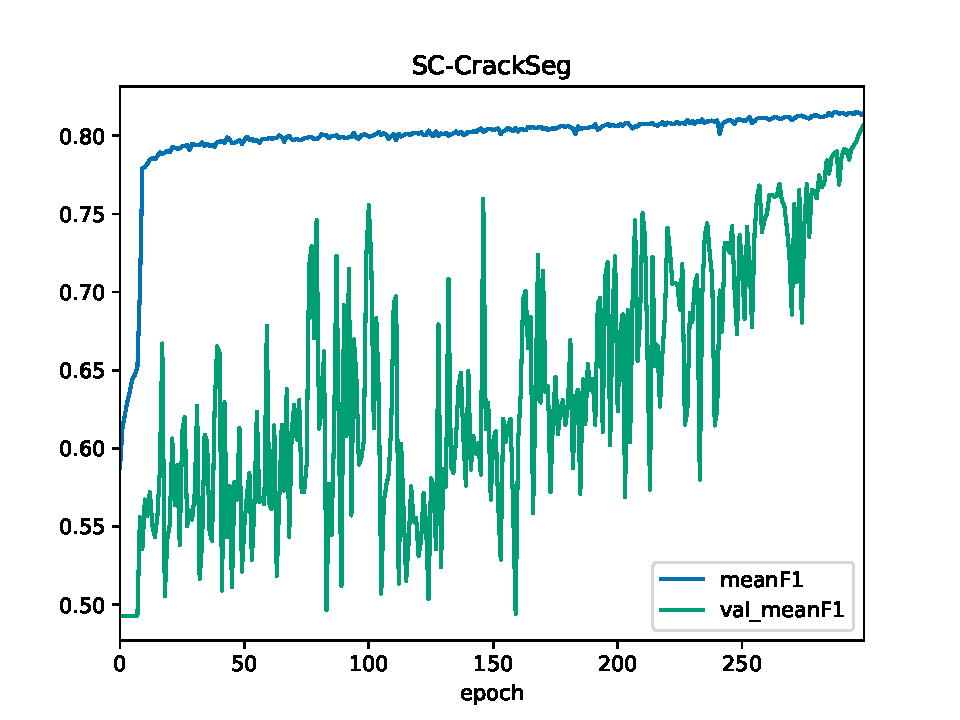
\includegraphics[width=0.3\textwidth]{res/crack-experiments-training-curves/sc-crackseg.pdf}   & 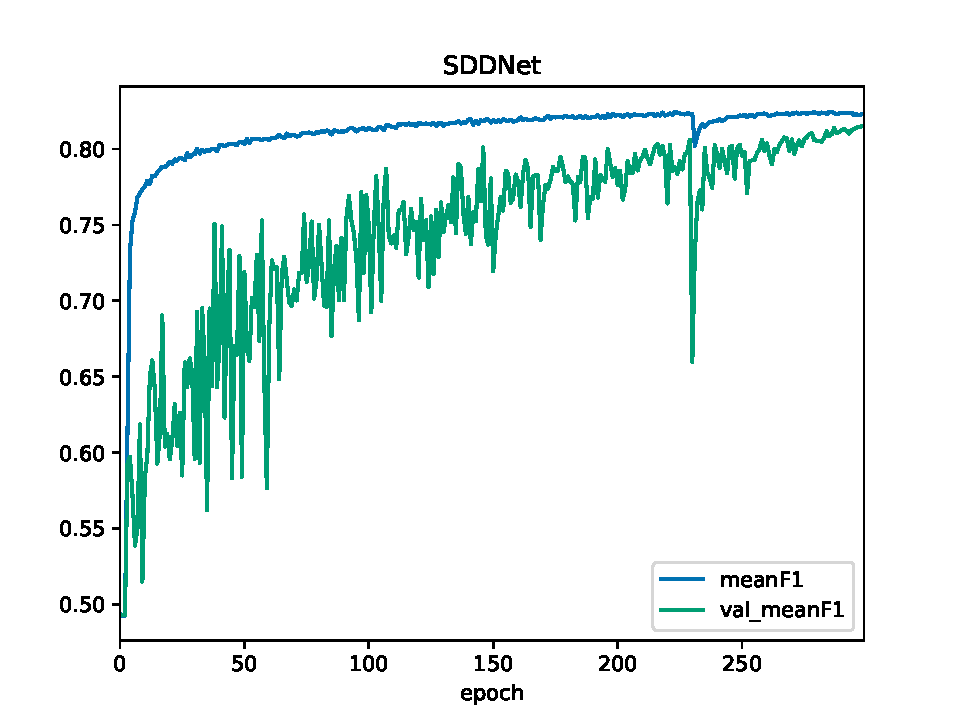
\includegraphics[width=0.3\textwidth]{res/crack-experiments-training-curves/sddnet.pdf}        & 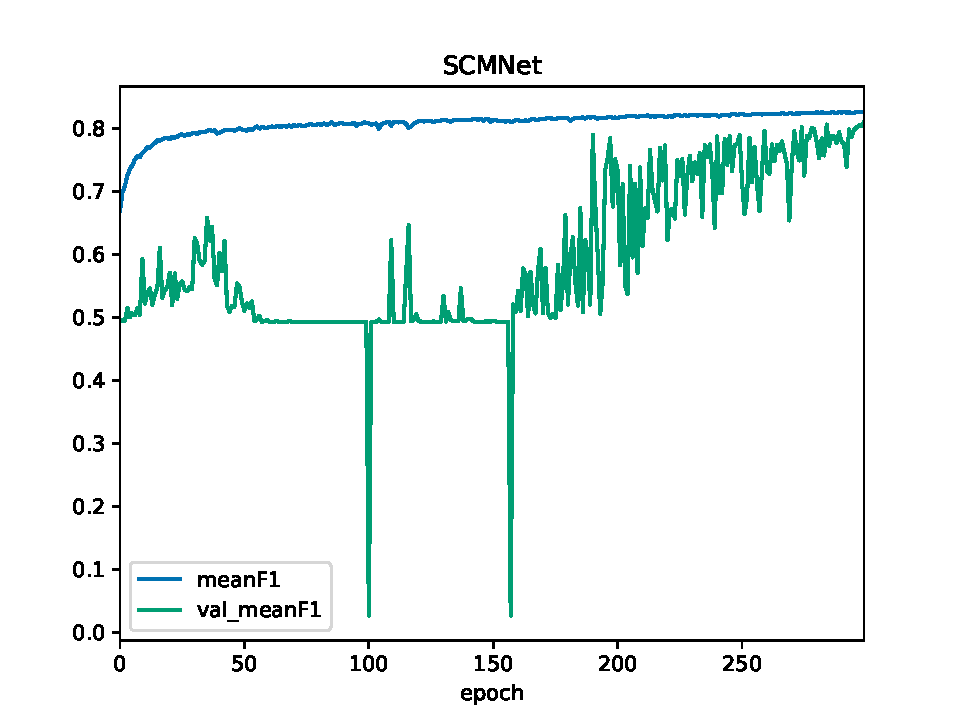
\includegraphics[width=0.3\textwidth]{res/crack-experiments-training-curves/scmnet.pdf}        \\
        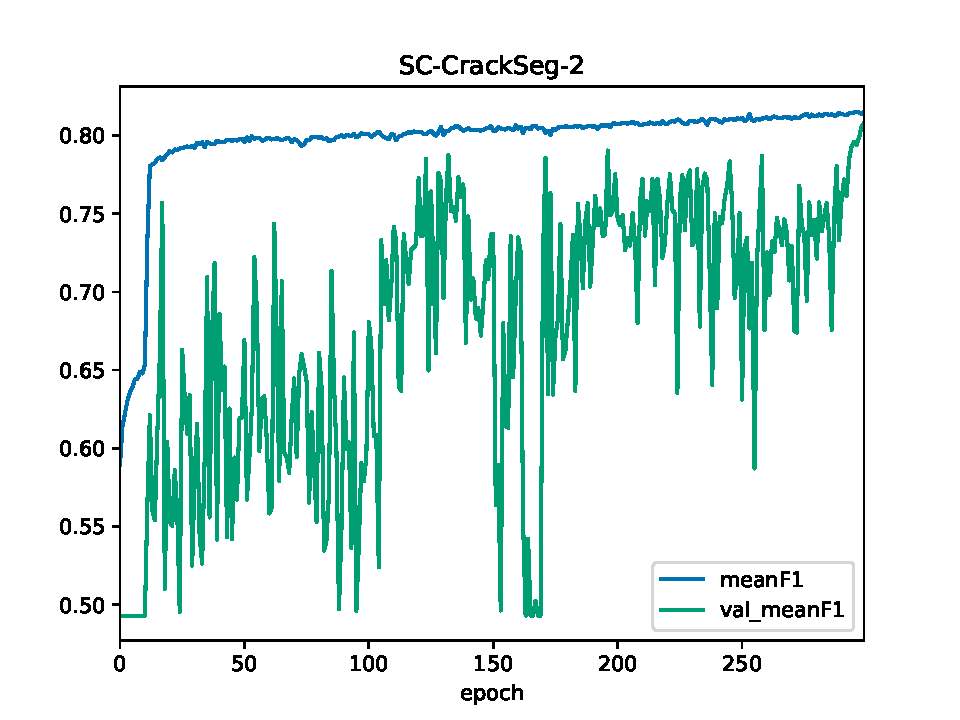
\includegraphics[width=0.3\textwidth]{res/crack-experiments-training-curves/sc-crackseg-2.pdf} & 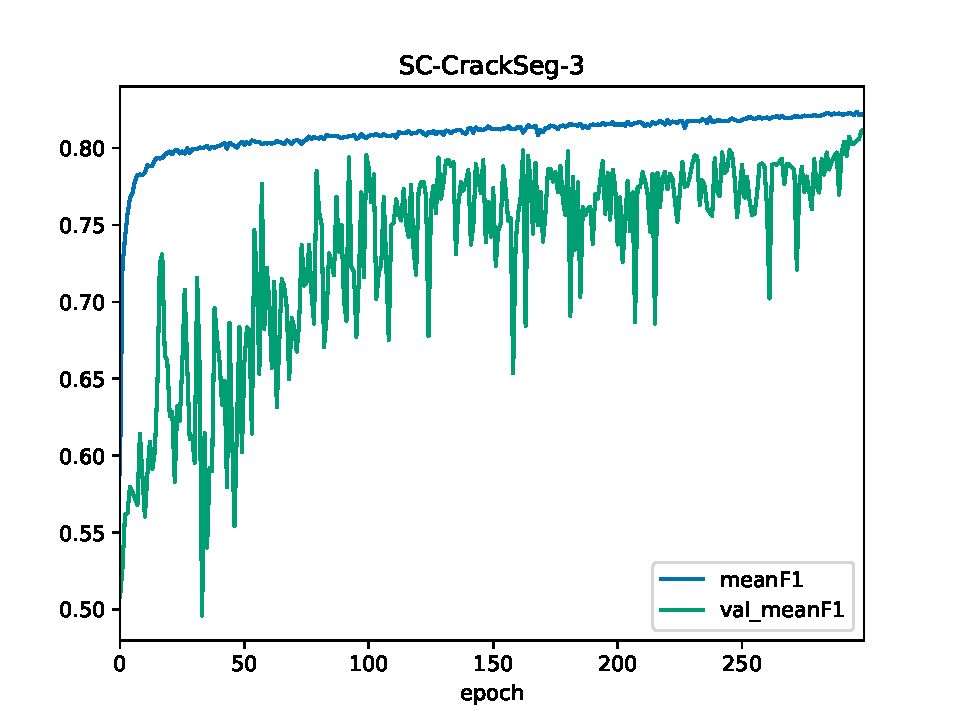
\includegraphics[width=0.3\textwidth]{res/crack-experiments-training-curves/sc-crackseg-3.pdf} & 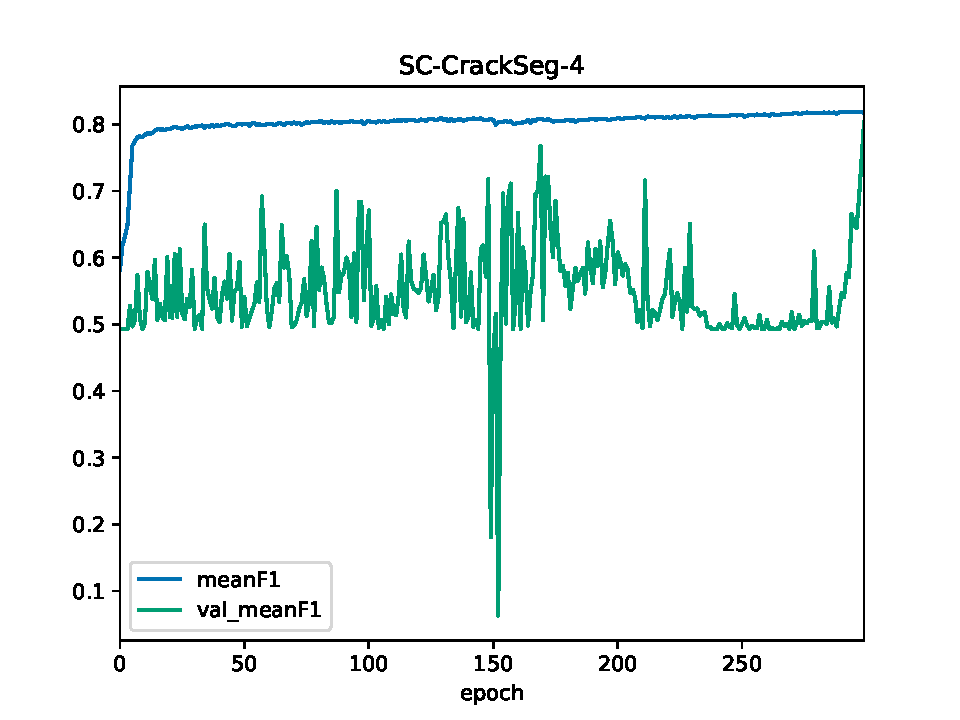
\includegraphics[width=0.3\textwidth]{res/crack-experiments-training-curves/sc-crackseg-4.pdf} \\
    \end{tabular}
    \caption{Train and test curves for SC-CrackSeg variations. Note the increased stability in models with DenSep modules (SDDNet, SC-CrackSeg-3, SC-CrackSeg-4).}
\end{figure}

Model stability also varied, with many models, especially SC-CrackSeg-2, often dropping in performance erratically during training. The introduction of the DenSep module appaeared to make models generally more stable. The larger models were, as expected, also more prone to overfitting.

Qualitative analysis (\autoref{fig:crackseg-experiment-qualitative}) revealed something interesting - only SDDNet and SC-CrackSeg-3 are capable of accurately segmenting specific crack boundaries. This performance does not appear to lead to major quantitative gains, but the distinction between "one crack" and "two cracks" could be significant in application context. SC-CrackSeg-3 may have this capability due to the enhanced global perspective provided by the deep branch and skip connections compared to SDDNet combined with the high-resolution detail provided by the skip connection, similarly to SDDNet.


\begin{figure}[htbp]
    \begin{tabular}{cccc}
        \begin{subfigure}[b]{0.23\textwidth}
            \centering
            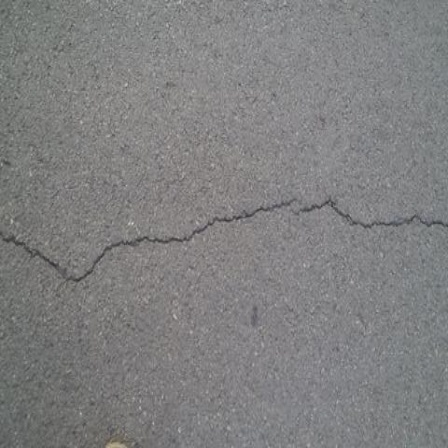
\includegraphics[width=\textwidth]{res/crackseg-experiment-qualitative/source.jpg}
            \caption{Source}
            \label{fig:crackseg-experiment-qualitative-source}
        \end{subfigure}
        \begin{subfigure}[b]{0.23\textwidth}
            \centering
            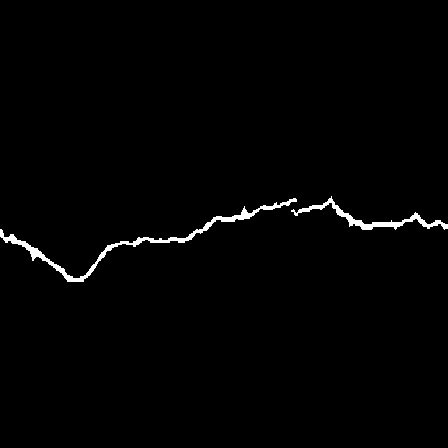
\includegraphics[width=\textwidth]{res/crackseg-experiment-qualitative/ground-truth.png}
            \caption{Ground Truth}
            \label{fig:crackseg-experiment-qualitative-ground-truth}
        \end{subfigure}
        \begin{subfigure}[b]{0.23\textwidth}
            \centering
            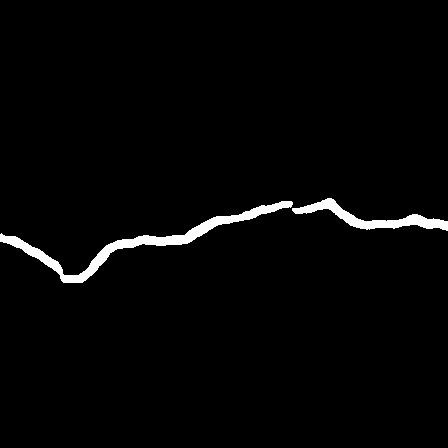
\includegraphics[width=\textwidth]{res/crackseg-experiment-qualitative/sddnet.png}
            \caption{SDDNet}
            \label{fig:crackseg-experiment-qualitative-sddnet}
        \end{subfigure}
        \begin{subfigure}[b]{0.23\textwidth}
            \centering
            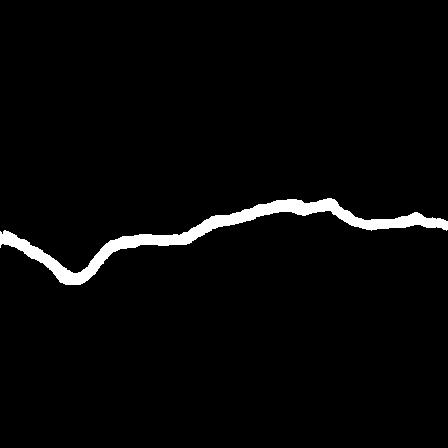
\includegraphics[width=\textwidth]{res/crackseg-experiment-qualitative/unet.png}
            \caption{U-Net}
            \label{fig:crackseg-experiment-qualitative-unet}
        \end{subfigure}
        \\
        \begin{subfigure}[b]{0.23\textwidth}
            \centering
            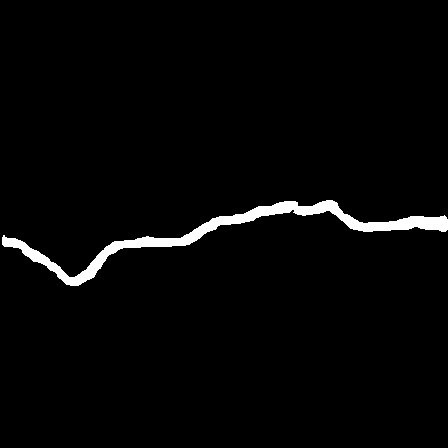
\includegraphics[width=\textwidth]{res/crackseg-experiment-qualitative/sc-crackseg.png}
            \caption{SC-CrackSeg}
            \label{fig:crackseg-experiment-qualitative-sc-crackseg}
        \end{subfigure}
        \begin{subfigure}[b]{0.23\textwidth}
            \centering
            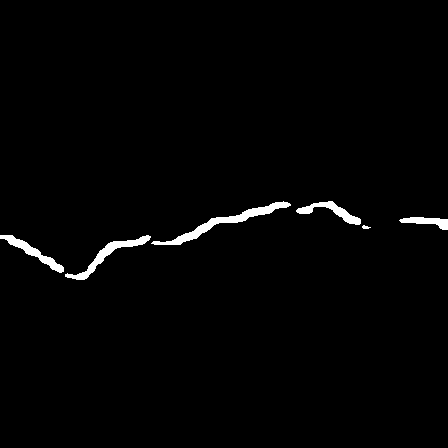
\includegraphics[width=\textwidth]{res/crackseg-experiment-qualitative/sc-crackseg-2.png}
            \caption{SC-CrackSeg-2}
            \label{fig:crackseg-experiment-qualitative-sc-crackseg-2}
        \end{subfigure}
        \begin{subfigure}[b]{0.23\textwidth}
            \centering
            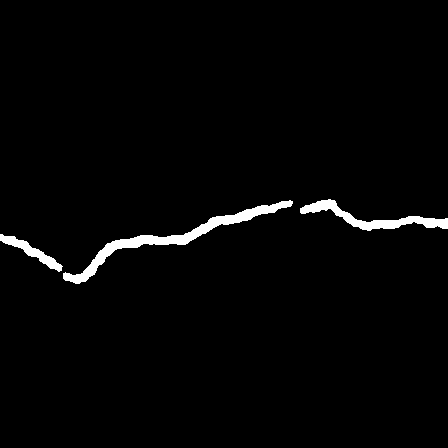
\includegraphics[width=\textwidth]{res/crackseg-experiment-qualitative/sc-crackseg-3.png}
            \caption{SC-CrackSeg-3}
            \label{fig:crackseg-experiment-qualitative-sc-crackseg-3}
        \end{subfigure}
        \begin{subfigure}[b]{0.23\textwidth}
            \centering
            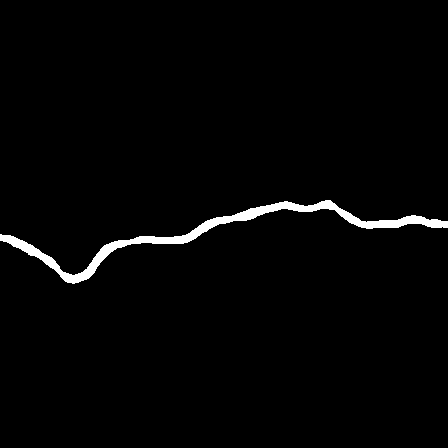
\includegraphics[width=\textwidth]{res/crackseg-experiment-qualitative/sc-crackseg-4.png}
            \caption{SC-CrackSeg-4}
            \label{fig:crackseg-experiment-qualitative-sc-crackseg-4}
        \end{subfigure}
    \end{tabular}
    \caption{Qualitative comparison of models on crack test set, displaying SC-CrackSeg-3 and SDDNet's ability to more finely segment crack components while maintaining quality.}
    \label{fig:crackseg-experiment-qualitative}
\end{figure}

Class balancing again achieved mixed success. While it initially appeared to have significant impact on performance, these were not consistent across experiments and random seeds. In fact, class imbalanced seemed to harm model performance in some areas, causing finely detailed crack segments to merged into a single large body (\autoref{fig:crackseg-class-balancing}). High class imbalance specifically seemed to reduce model performance significantly.

\begin{figure}[htbp]
    \centering
    \begin{tabular}{ccc}
        \begin{subfigure}[b]{0.3\textwidth}
            \centering
            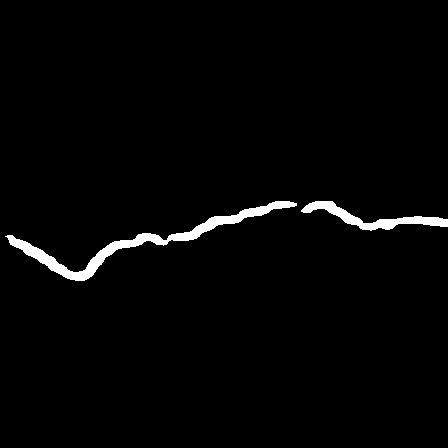
\includegraphics[width=0.75\textwidth]{res/class-balancing-comparison/sc-crackseg-none}
            \caption{None}
            \label{fig:crackseg-class-balancing-none}
        \end{subfigure}
        \begin{subfigure}[b]{0.3\textwidth}
            \centering
            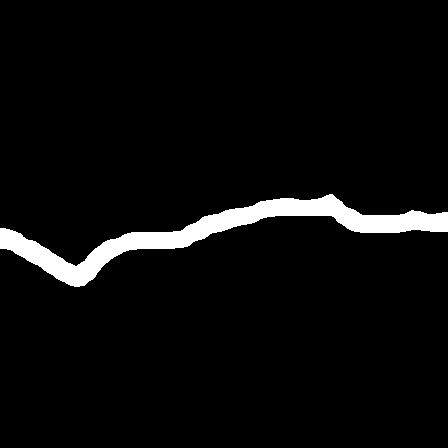
\includegraphics[width=0.75\textwidth]{res/class-balancing-comparison/sc-crackseg-low}
            \caption{Low}
            \label{fig:crackseg-class-balancing-low}
        \end{subfigure}
        \begin{subfigure}[b]{0.3\textwidth}
            \centering
            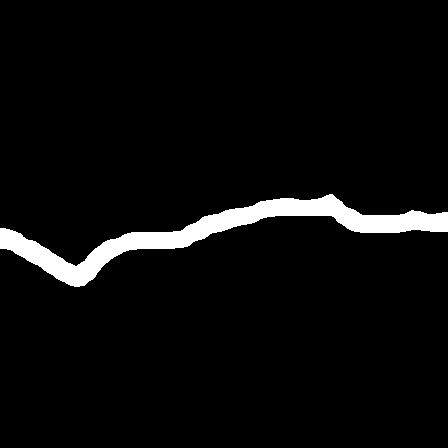
\includegraphics[width=0.75\textwidth]{res/class-balancing-comparison/sc-crackseg-high}
            \caption{High}
            \label{fig:crackseg-class-balancing-high}
        \end{subfigure}
    \end{tabular}
    \caption{Qualitative comparison of different levels of class balancing. Low balancing has class weights as $0.8:0.2$ for crack$:$non-crack respectively. High balancing has class weights as the inverse proportion of class frequency in the training set.}
    \label{fig:crackseg-class-balancing}
\end{figure}

\subsubsection*{Ablation study}

Modifications in SC-CrackSeg-2 and SC-CrackSeg-3b were ablated. SC-CrackSeg-3b performed surprisingly strongly without the additional skip connection, though it still helps to improve performance and stabilises the model. SC-CrackSeg-2 originally contained more channels and additional layers in the shallow branch to increase processing of fine details, but ablation identified this increased complexity was unnecessary.

\begin{table}[h]
    \resizebox{\textwidth}{!}{%
        \begin{tabular}{|r|r|l|r|l|l|}
            \hline
            \multicolumn{1}{|l|}{\textbf{\begin{tabular}[c]{@{}l@{}}Deep \\ Conv \\ Layers/Set \\ Removed\end{tabular}}} & \multicolumn{1}{l|}{\textbf{\begin{tabular}[c]{@{}l@{}}Shallow \\ Conv \\ Layers/Set \\ Added\end{tabular}}} & \textbf{\begin{tabular}[c]{@{}l@{}}Reduced \\ Max\\ Channels\end{tabular}} & \multicolumn{1}{l|}{\textbf{Val mF1}} & \textbf{FLOPS} & \textbf{Parameters} \\ \hline
            0                                                                                                            & 0                                                                                                            &                                                                            & 0.807                                 & 1.4M           & 1.27M               \\ \hline
            1                                                                                                            & 0                                                                                                            &                                                                            & \textbf{0.808}                        & 1.22M          & 0.97M               \\ \hline
            0                                                                                                            & 1                                                                                                            &                                                                            & 0.798                                 & 1.42M          & 1.31M               \\ \hline
            1                                                                                                            & 1                                                                                                            &                                                                            & \textbf{0.808}                        & 1.24M          & 1.01M               \\ \hline
            2                                                                                                            & 0                                                                                                            &                                                                            & 0.799                                 & \textbf{1.14M} & \textbf{0.7M}       \\ \hline
            1                                                                                                            & 0                                                                                                            & Yes                                                                        & 0.807                                 & 1.19M          & 0.81M               \\ \hline
        \end{tabular}

        \quad

        \begin{tabular}{|l|l|r|l|l|}
            \hline
            \textbf{Skip Connection} & \textbf{DenSep Module} & \multicolumn{1}{l|}{\textbf{Val mF1}} & \textbf{FLOPS} & \textbf{Parameters} \\ \hline
                                     &                        & 0.807                                 & \textbf{1.4M}  & \textbf{1.27M}      \\ \hline
            Yes                      &                        & 0.809                                 & 1.44M          & 1.28M               \\ \hline
                                     & Yes                    & 0.811                                 & 2.12M          & 1.5M                \\ \hline
            Yes                      & Yes                    & \textbf{0.812}                        & 2.16M          & 1.51M               \\ \hline
        \end{tabular}
    }
    \caption{Ablation study of SC-CrackSeg-2 (left) and SC-CrackSeg-3 (right). The final SC-CrackSeg-2 variation was chosen as it provided a strong balance between model efficiency and performance.}
    \label{cap:sc-crackseg-ablation}
\end{table}

\subsection*{Conclusions}

While conventional wisdom often states the strongest machine learning architectures are general, crack segmentation is an interesting example of a scenario where specifically tuned architectures can be valuable. SC-CrackSeg and its variations make select sacrifices in areas minimally impactful towards performance and apply specific optimisations for the crack segmentation task.

The lack of class balancing's effect is surprising, particularly due to effectiveness observed in other papers \cite{liu_deepcrack_2019}. It appears the effect of class imbalance is model and scenario-dependent in crack segmentation. Perhaps more effect would have been observed in a more complex task than crack segmentation where a larger number of classes must be balanced. In crack segmentation, predicting further crack pixels is often the only way to further reduce loss, since there are only two classes.

We further discover the extreme effectiveness of SDDNet. DenSep blocks are simple, possess few parameters, and yet achieve extremely strong performance. Introduction of these blocks increases model stability and, when applied properly, the performance of SC-CrackSeg. In general, our experiments confirm that increased complexity is not necessary for the crack segmentation task, and may even be a hindrance, producing instability and overfitting. Though SDDNet is effective, our own SC-CrackSeg models may prove more effective in scenarios where computation count and model size.

In general, the lack of difference between widely varying architectures was surprising - many model's top F1 scores were within 0.01 of each other, despite varying qualitative results. This indicates there are further metrics in the crack segmentation task (such as number of cracks detected) not covered by traditional qualitative metrics, and that performance in terms of qualitative metrics has been largely saturated using the chosen architectures.

Ultimately, we introduce a number of competitive crack segmentation architectures in SC-CrackSeg and it's variations. We explore the effects of different architectural and external choices on performance in the context of crack segmentation.

\section{Future work}
\begin{itemize}
    \item \textbf{Simpler architecture} - the results compared to SDDNet indicate SC-CrackSeg's architecture may still be fundamentally too complex. Simplifying branches (as in ContextNet \cite{poudel_contextnet_2018} to Fast-SCNN \cite{poudel_fast-scnn_2019}) may result in significant cost reductions.
    \item \textbf{Additional metrics} - Certain qualitative-level metrics may be needed to further develop meaningful improvements and comparisons in the crack segmentation space. These could include the number of cracks detected and the number of false positives, for instance.
\end{itemize}

% ------------------------------------------------------------------------------
% Unsupervised Domain Adaptation for Segmentation
% ------------------------------------------------------------------------------
\chapter{Adversarial Domain Adaptation for Transformer Segmentation}

Transformers are known for their high domain-adaptive potential. In this chapter, we explore the usage of the SegFormer \cite{xie_segformer_2021} transformer segmentation network to the unsupervised domain adaptation task. We do so using the common domain-adversarial approach to semantic segmentation, the effectiveness of which has not previously been assessed in this context.

\section{Background}

\subsection{Unsupervised domain adaptation}
Unsupervised Domain Adaptation (UDA) fundamentally seeks to address the lack of high-quality training data for specific machine learning tasks. A subset of transfer learning, domain adaptation explores how to transfer knowledge learned on a labelled source domain to an unlabelled target domain, where the two domains possess the same label space but contain a domain shift. This shift may be small (e.g. one city to another) or large (e.g. synthetic to real data). Formally, consider a source dataset $D_S$ consisting of inputs $X_S$ and labels $Y_S$ as samples from an overall distribution $P_S$. Similarly, a target set $D_T$ consists of images $X_T$ from a distribution $P_T$. Critically, the labels, $Y_T$, are not available. Due to the domain shift between the datasets, we can intuit $P_T \neq P_S$, but that $P_S$ will be a strong starting point for learning $P_T$ due to the similarity of the domains. UDA, then, involves strategies for moving from $P_S$ to $P_T$ \cite{wilson_survey_2020}, unsupervised labels for our true desired target $P_T$ are not available.

Many fundamentally different approaches to domain adaptation exist. Two in particular have become relevant to semantic segmentation: domain-adversarial learning and self-training. Domain adversarial learning is a subset of domain invariant feature learning \cite{wilson_survey_2020}, a UDA approach based on the intuition that a model will be more successful if producing on features similar to those it was trained on. In other words, this UDA approach improves performance by encouraging the model to produce features from the target set similar to those in the source set. This is usually achieved by adding another parameter to the model loss, such as the statistical distance between the source and target model's feature distributions \cite{gretton_kernel_2006} \cite{sun_return_2015}. Recently, many works \cite{ganin_unsupervised_2015} \cite{ganin_domain-adversarial_2016} instead implement an adversarial \cite{goodfellow_generative_2014} approach. One model is trained on the source/target dataset tasks, while another, the discriminator, takes features from the former as input and is trained to classify whether the features belong to the source or target dataset. The discriminator's loss is then negated and added to the original model's loss, training it to "trick" the discriminator. The intuition here is that producing source and target features that a neural network cannot distinguish is a more effective means of ensuring their similarity than traditional distances. This approach is known as domain adversarial learning \cite{ganin_domain-adversarial_2016}.

\begin{figure}[h]
    \centering
    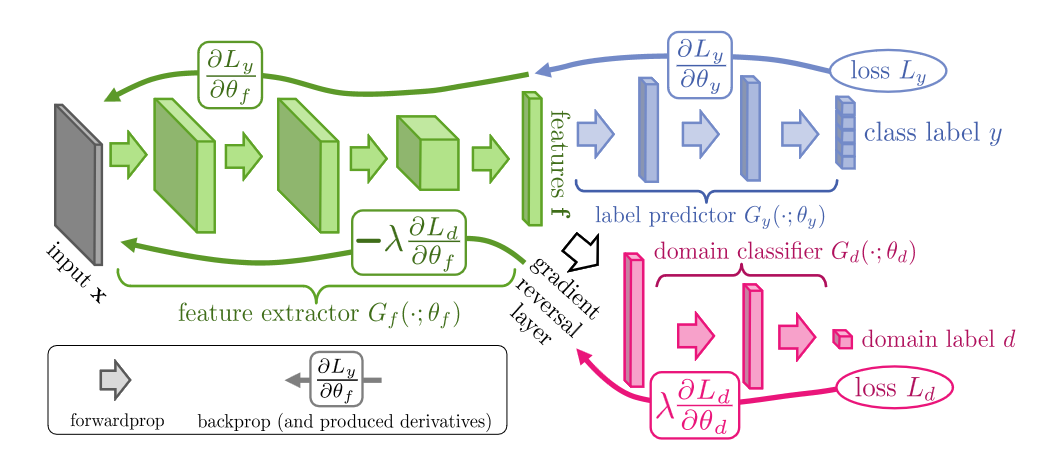
\includegraphics[width=0.67\textwidth]{res/domain-adversarial-training.png}
    \caption{Representation of domain adversarial training, retrieved from
        \cite{ganin_domain-adversarial_2016}}
    \label{fig:domain-adversarial-training}
\end{figure}

Self-training, or pseudo-labelling, is another common approach. Its intuition is that the highest quality, most "confident" predictions made by a source-trained model on target data will provide more valuable than non-valuable knowledge to the model \cite{wilson_survey_2020} \cite{kamnitsas_transductive_2021}. In essence, the source-trained model makes predictions on target samples, the most confident of these predictions - known as pseudo-labels - are added to the training set, and the cycle is repeated. How the confidence of a model is determined varies. Some studies use ensemble approaches \cite{kamnitsas_transductive_2021}, though many semantic segmentation techniques use the magnitude of a model's softmax output as a measure of confidence, where a greater softmax value is a more confident prediction \cite{zou_domain_2018}.

\subsection{Transformers for semantic segmentation}

The transformer architecture revolutionised the deep learning field in 2017 \cite{vaswani_attention_2017}. Initially applied for sequence-based natural language processing (NLP) tasks, transformers propose a fundamentally different approach to CNNs. Transformers are based on the concepts of self-attention and multi-head attention. These respectively give the model the ability to determine importance between different components o fa sequence, and compute this importance in a number of different ways, similar to having multiple filters for different features in CNNs. ViT \cite{dosovitskiy_image_2021} was the first attempt to produce a fully transformer-based vision architecture (as in \cite{vaswani_attention_2017}) modified for image inputs. Rather than encoding each pixel into an input sequence (which would be prohibitively expensive), ViT groups the input image into $16 \times 16$ patches for encoding into the input sequence. Transformers became ubiquitous in NLP due to their ability to map long-distance relationships and their extreme scalability with increasing amounts of data \cite{devlin_bert_2019} \cite{radford_language_2019}. However, transformers lack the translational equivariance and locality that are believed to make CNNs so effective for vision, and experiments indeed showed that ViT is outperformed by state-of-the-art CNNs when trained on smaller datasets. However, when trained on extremely large datasets, the scalability of transformers appears to win out against these biases.

\begin{figure}[h]
    \centering
    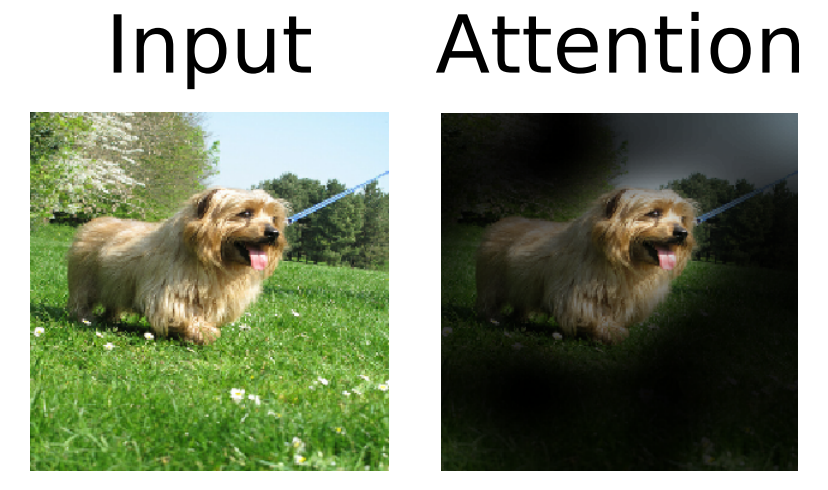
\includegraphics[scale=0.5]{res/vit-attention.png}
    \caption{Visualisation of self-attention for images in ViT \cite{dosovitskiy_image_2021}. Brighter pixels had greater importances computed between them by the transformer.}
    \label{fig:vit_attention}
\end{figure}

Other models have since built on ViT. Most significantly for segmentation, Pyramid Vision Transformer (PVT) \cite{wang_pyramid_2021} modifies ViT to be more suitable for dense prediction, implementing $4 \times 4$ instead of $16 \times 16$ image patches for increased feature detail. To maintain performance and develop multi-scale features, it then progressively merges patches between transformer blocks. DeIT \cite{touvron_training_2021} proposes a student-teacher and distilled training approach that allows ViT’s architecture to perform strongly even when pre-trained on far smaller datasets. Swin Transformer \cite{liu_swin_2021} builds hierarchical feature maps like PVT by merging image patches, but only computes self-attention within each window for efficiency. Twins \cite{chu_twins_2021} combines locally-grouped and global self-attention to achieve state-of-the-art performance. SETR \cite{zheng_rethinking_2021} uses an encoder-decoder architecture with a pre-trained vision transformer (such as ViT or DeIT) as a backbone, and found pre-training was essential. Without pre-training, SETR achieved only 42\% mIoU on Cityscapes, worse than models with 1\% the parameters \cite{paszke_enet_2016}. However, with pre-training, SETR achieved a state-of-the-art 82.15\% mIoU on Cityscapes.

\bigbreak
\begin{figure}[h]
    \centering
    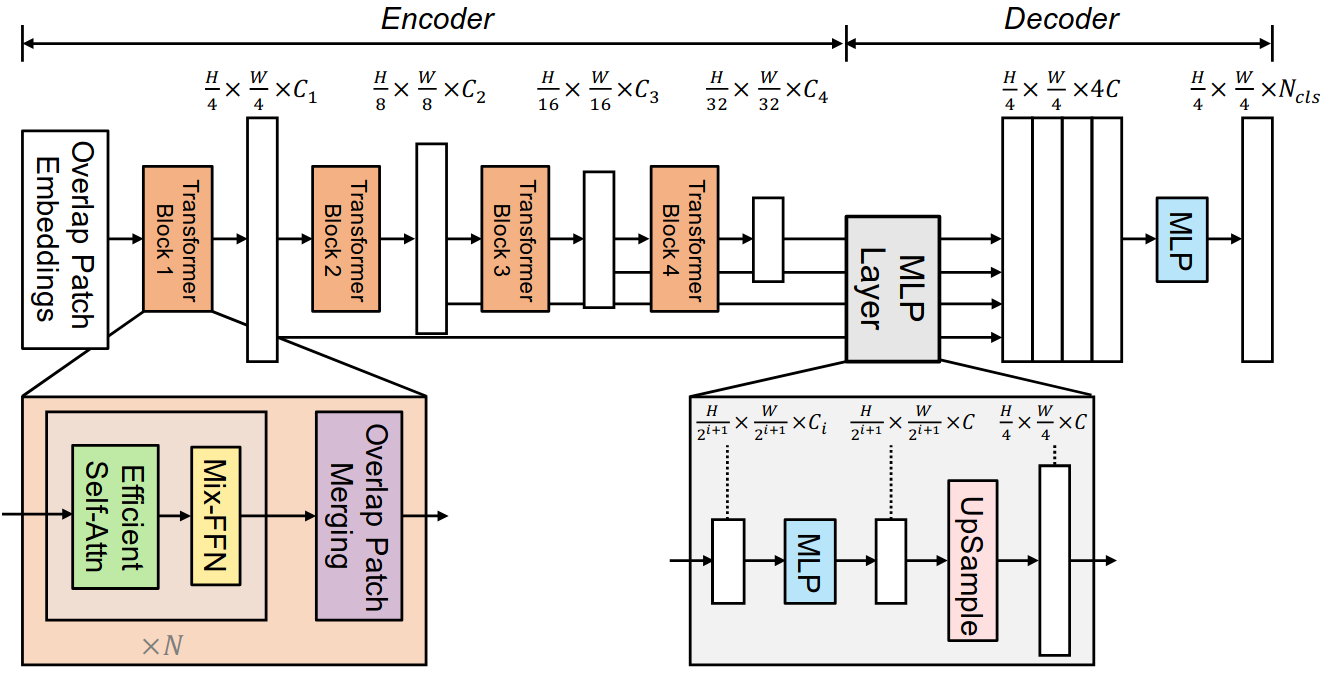
\includegraphics[width=0.8\textwidth]{res/segformer-architecture.png}
    \caption{Architecture of SegFormer \cite{xie_segformer_2021}.}
    \label{fig:das-discriminators-output}
\end{figure}

SETR demonstrated the capacity of transformers in segmentation, but was limited by its use of a backbone designed for classification. SegFormer \cite{xie_segformer_2021} addressed a number of these issues using it’s Mix Transformer Encoder (MiT). First, dense $4 \times 4$ pixel patches and progressive patch merging are used as in PVT \cite{wang_pyramid_2021}. Rather than pure-MLP layers after each attention block, SegFormer employs MLPs mixed with $3 \times 3$ convolutions without zero-padding. This leaks spatial spatial information to the model that bypasses the need for positional encoding. Combined with a simple all-MLP encoder, possible due to the transformer’s receptive field, SegFormer achieves a state-of-the art 51.0\% mIoU on the new, challenging ADE20K dataset \cite{zhou_semantic_2018}.

\subsection*{UDA for semantic segmentation}

Both domain adversarial and self-training approaches have been applied to semantic segmentation, but must be adjusted due to the increased complexity of dense prediction. It is also critical to consider that semantic segmentation requires many predictions to be made per input, rather than a single one as in classification. \cite{hoffman_fcns_2016} was first in domain adversarial approaches, using FCN with a discriminator that took in feature space in "patches", where each patch represented the size of the model's receptive field. It was found passing all dense features to the discriminator simultaneously marginalised fine-grained detail in output predictions. This was addressed via a class distribution loss to encourage learning of rare classes. On the contrary, \cite{tsai_learning_2020} use an output-level discriminator combined with multiple feature-level discriminators, intuiting that the complex output space of segmentation should look similar between approaches. FADA \cite{wang_classes_2020} applies a fine-grained discriminator that produces class-wise logits to encourage the model to effectively transfer each class. \cite{michieli_adversarial_2020} combines a pixel-wise adversarial approach with self-training.

Self-training approaches have produced many state-of-the art results. Many contributions were made in \cite{zou_domain_2018}, who apply pseudo-labelling to segmentation by masking out (making the model ignore) all but the $r\%$ most confident correct pixel predictions in each image. Confidence is measured using softmax magnitude. A scheduling system is introduced to gradually increase $r$ as target predictions become more reliable. Class-balancing is also introduced to counteract the domination of easy-to-predict classes. ADVENT \cite{vu_advent_2019} found focusing training on low-confidence regions could boost performance, and \cite{li_bidirectional_2019} combines pseudolabelling with GAN image translation.

\subsection*{Vision transformers in UDA}

Transformers are known to have extremely strong transfer learning capabilities \cite{radford_language_2019} \cite{wright_transformer_2020}. This extends to vision, where ViT \cite{dosovitskiy_image_2021} and SETR \cite{zheng_rethinking_2021} identified the effectiveness of pre-training on a large dataset like ImageNet before adapting to labelled segmentation data. Transferrable Vision Transformer (TVT) \cite{yang_tvt_2021} was the first to explore the domain adaptation abilities of vision transformers specifically, but did so in the classification space using ViT. It was found that ViT's zero-shot transferability outperformed many state-of-the-art CNN-based techniques for domain adaptation. This was built on using an adversarial patch-wise discriminator that de-emphasises easy-to-disciminate patch weights, combined with a loss that maximises feature clustering \cite{chapelle_semi-supervised_2005}. Patch-wise feature alignment was also applied in \cite{wang_exploring_2021} for object detection.

\subsection*{DAFormer}

The domain transferability of general vision transformers and the state-of-the art performance of segmentation transformers like SegFormer \cite{xie_segformer_2021} had both been established by early 2022. However, there had been no exploration into combining these strengths.
Our intuition was that, just as vision transformers outperformed existing domain transfer approaches even with naive examples, a similar boost of performance could be achieved by segmentation transformers.

An intuitive approach to this problem would be to apply a model like SegFormer to UDA, first evaluating its performance in a naive setting (train on source, evaluate on target) and then using an approach tailored to domain adaptation. To avoid having to interact with many of the complexities brought on by moving from a convolutional to transformer architecture, a largely architecture-independent approach proven for segmentation, such as self-training \cite{zou_domain_2018} may be preferable. While this was the initial plan for this chapter of the thesis, it was also unfortunately the precise subject of the 2022 paper DAFormer \cite{hoyer_daformer_2022}. DAFormer identifies the extreme domain-adaptive capacity of SegFormer and improves it for the purposes of UDA. It does so by modifying the SegFormer backbone, applying class balancing, and adding novel regularisation techniques such as distribution distance from features trained on the generic ImageNet dataset. As we sought to explore novel concepts and approaches, we instead shifted focus onto the other popular means of performing domain adaptation - domain-adversarial training. Domain adversarial approaches were not explored in DAFormer due to the recent success of self-training in other research and the difficulty of implementing domain adversarial methods in segmentation transformers. The challenge comes primarily from the large changes that must be made to the training pipeline - adding a peripheral network with a separate training goal - and the large number of peripheral network setups.

\section{Domain Adversarial SegFormer}

We here describe the experimental setup for Domain Adversarial SegFormer (DAS). Fundamentally, DAS follows the discriminator-based adversarial domain adaptation approach. Our system is trained two-fold: firstly, we perform conventional training by making our segmentation model, consisting of feature-extractor $F$ and classifier $C$, make predictions on samples $X_S$ from our source dataset, then using its labels $Y_s$ to produce the segmentation loss $\mathcal{L}_{seg}$. We then apply an adversarial discriminator $D$ to the features produced by the feature-extractor on source samples $X_S$ and unlabelled target samples $X_T$. This discriminator attempts to classify input features as belonging to the source or target distribution, and is evaluated to produce the discriminator loss $\mathcal{L}_{disc}$. The loss of the discriminator is then used to encourage the segmentation model, in theory pushing it to produce domain-invariant features and thus perform more strongly on the target set. This process can be thought of as alternately optimising the following two objectives:

\begin{itemize}
    \item Segmentation Network: $C(F(X_S)), D(F(X_S)), F(X_T) \rightarrow \mathcal{L}_{seg} - \mathcal{L}_{disc} $
    \item Discriminator: $D(F(X_S)), F(X_T) \rightarrow \mathcal{L}_{disc}$
\end{itemize}

We train both models in an end-to-end manner using a gradient reversal layer (GRL) \cite{ganin_domain-adversarial_2016}. The gradient is reversed at the beginning of the feature extractor, meaning backpropagation can simply be performed on $\mathcal{L}_{seg} + \mathcal{L}_{disc}$. This will encourage the discriminator to minimise domain classification error, while, upon gradient reversal, encouraging the segmentation model to maximise the domain classification error. The adaptation factor $\lambda$ scales the gradient as it moves through the GRLs - this can be used to reduce the effect of the discriminator loss on the segmentation model while still allowing the discriminator to learn effectively.

% \pagebreak
% \hspace*{1mm}
\bigbreak
\begin{lstlisting}[language=Python, caption=Gradient reversal function implemented in PyTorch \cite{paszke_pytorch_2019}. Based on \url{https://github.com/tadeephuy/GradientReversal}]
class GradientReversalFunction(Function):
    """Gradient reversal function. Acts as identity transform during forward pass, 
    but multiplies gradient by -da_lambda during backpropagation. this means da_lambda 
    effectively becomes the loss weight during training.
    """
    @staticmethod
    def forward(ctx, x, da_lambda):
        ctx.save_for_backward(x, da_lambda)
        return x
    
    @staticmethod
    def backward(ctx, grad_output):
        grad_input = None
        _, da_lambda = ctx.saved_tensors
        if ctx.needs_input_grad[0]:
            grad_input = - da_lambda*grad_output
        return grad_input, None

    revgrad = GradientReversalFunction.apply
\end{lstlisting}

For our experiments, we use SegFormer-B3 \cite{xie_segformer_2021} pre-trained on ImageNet as a backbone. While DAFormer uses the larger MiT-B5 backbone, introducing the domain discriminator increases the parameters (and therefore memory requirement) of the experimental setup, which we address by using a smaller backbone to compare results. Our SegFormer backbone is pre-trained on the ImageNet dataset. Pre-training is critical to the performance of transformers, especially in terms of domain adaptivity \cite{dosovitskiy_image_2021}. Consequently, we do not change the backbone structure as part of our experiments as this would complicate the use of the pre-trained weights.

DAS is built upon the DAFormer \cite{hoyer_daformer_2022} repository \footnote{\url{https://github.com/lhoyer/DAFormer}}, which itself is built upon the MMSegmentation Repository \footnote{\url{https://github.com/open-mmlab/mmsegmentation}} (version 0.16.0). We use this codebase as a baseline for our work to allow for improved accessibility to the project and interoperability with other research, as all MMSegmentation projects are structured and developed in the same way. In this work, we effectively engineer modular extensions to the MMSegmentation repository that permit domain adversarial training. To demonstrate the flexibility of the platform, we develop domain adversarial models not only using SegFormer, but also DeeplabV3+ \cite{chen_encoder-decoder_2018}.

The repository containing the code is hosted publicly on GitHub \footnote{\url{https://github.com/Moritz-Bergemann/domain-adversarial-segformer}}. Detailed steps to reproduce the training environment can be found in the repository README.

\subsection{Explored Iterations}
To effectively assess the effect of domain adversarial training when using segmentation transformers, we compare various adversarial discriminators and adversarial approaches.

\subsubsection{Basic feature discriminator}
The basic feature discriminator (as deployed in \cite{hoffman_fcns_2016}) takes the SegFormer encoder's features as input to make domain classification. The input features are in the $H \times W \times C$ non-patch-embedded format, similar to the input of many existing discriminators.

We implement a linear discriminator, consisting of 3 linear layers, mirroring SegFormer's simple decoder. We hope this allows the discriminator to learn from features that have been learned by the feature extractor for this structure.

Additionally, we also implement a more traditional convolutional discriminator, consisting of 2 convolutional layers before global average pooling.

\bigbreak
\begin{figure*}[h]
    \centering
    \begin{subfigure}[b]{\textwidth}
        \centering
        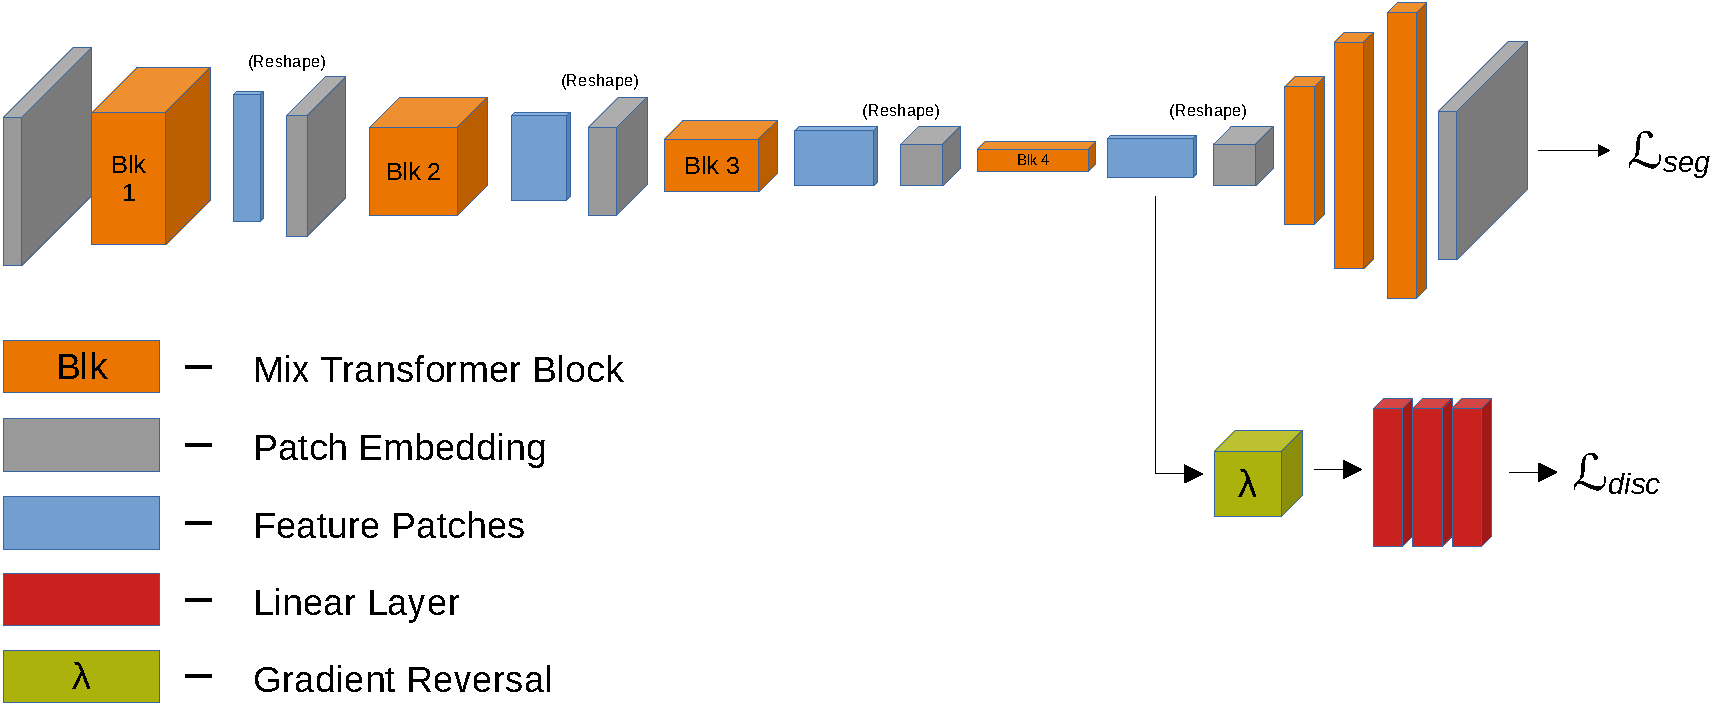
\includegraphics[width=0.6\textwidth]{res/discriminator-diagrams/linear.pdf}
        \label{fig:das-discriminators-linear}
    \end{subfigure}
    \begin{subfigure}[b]{\textwidth}
        \centering
        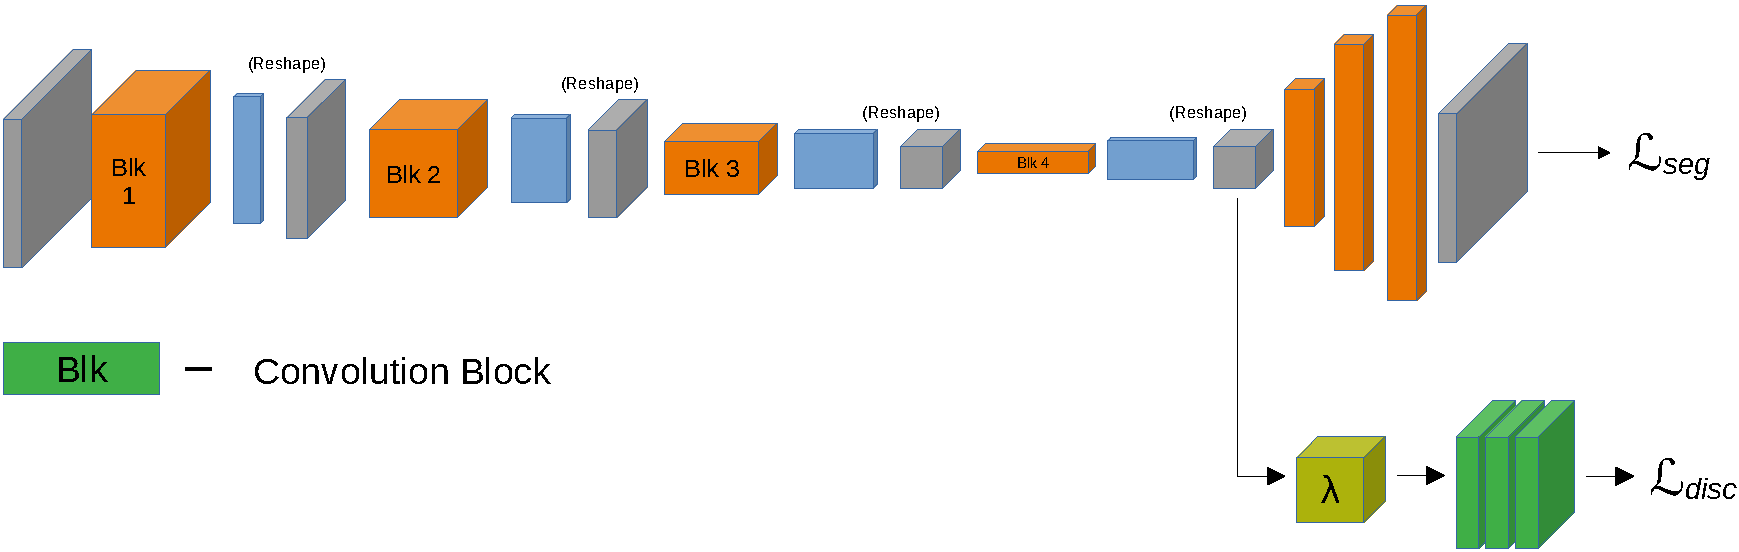
\includegraphics[width=0.6\textwidth]{res/discriminator-diagrams/convolutional.pdf}
        \label{fig:das-discriminators-conv}
    \end{subfigure}
    \caption{Architectures of linear (top) and convolutional (bottom) DAS discriminator architectures. Note the linear discriminator retrieves features from patch embeddings, while the convolutional retrieves them from the $H \times W \times C$ transformed features.}
    \label{fig:das-discriminators}
\end{figure*}

\subsubsection{Output discriminator}

Based on \cite{tsai_learning_2020}, we introduce a convolutional discriminator on the output space. While slightly different to the feature-level discriminators, the intuition here is similar - the structure of segmentation output produced from the source and target domains should be similar. Similar to Tsai et. al. \cite{tsai_learning_2020}, we use a convolutional discriminator with 6 layers, which takes the segmentation logits as input.

\bigbreak
\begin{figure}[h]
    \centering
    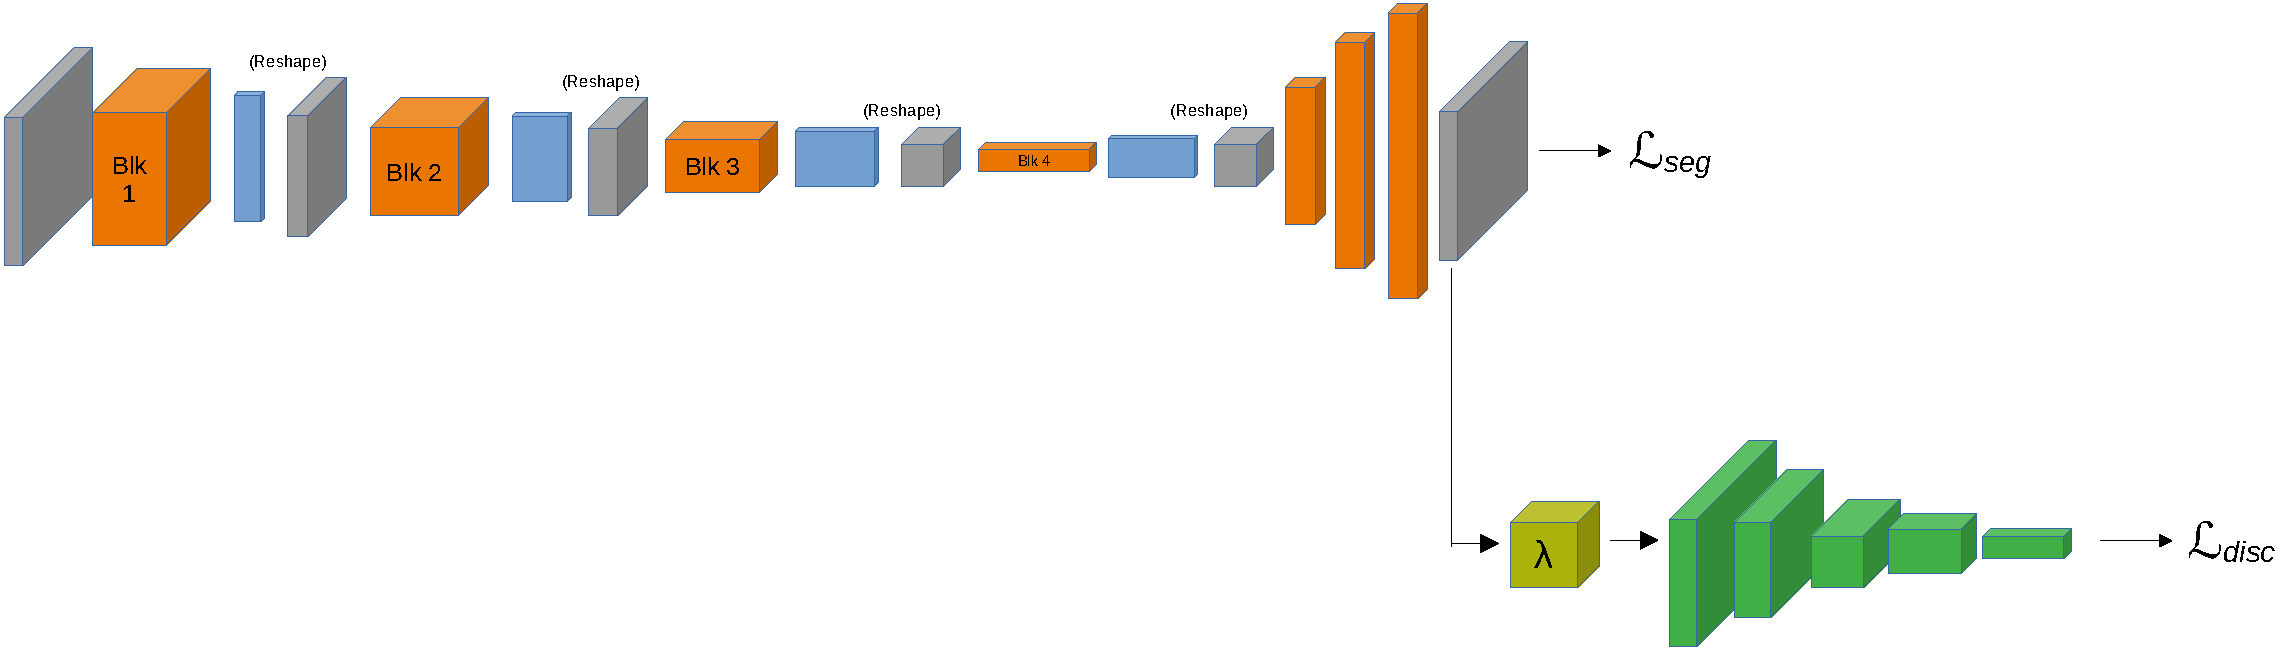
\includegraphics[width=0.8\textwidth]{res/discriminator-diagrams/dcgan-output.pdf}
    \caption{Architecture of convolutional DCGAN-like discriminator.}
    \label{fig:das-discriminators-output}
\end{figure}


\subsubsection{Patch-wise discriminator}
The patch-wise discriminator seeks to take specific advantage of the transformer architecture. As with TVT \cite{yang_tvt_2021}, we intuit that embedded patches within the transformer's self-attention represent different aspects or features of the input image. Therefore, we can apply discriminators to each patch individually to ensure feature components are domain indiscriminate without marginalising out distribution information.

In the conventional patch-wise discriminator, all features are passed in sequence to the same discriminator. In a further effort to avoid marginalising class distribution, we deploy a unique patch-wise discriminator, where each patch position (which we intuit to possess similar kinds of features across different inputs) receives its own discriminator with separate weights.

To maintain structure simple and similar to the rest of the transformer, each patch-wise discriminator consists of 3 linear layers, applied along patch channels.

\bigbreak
\begin{figure*}[h]
    \centering
    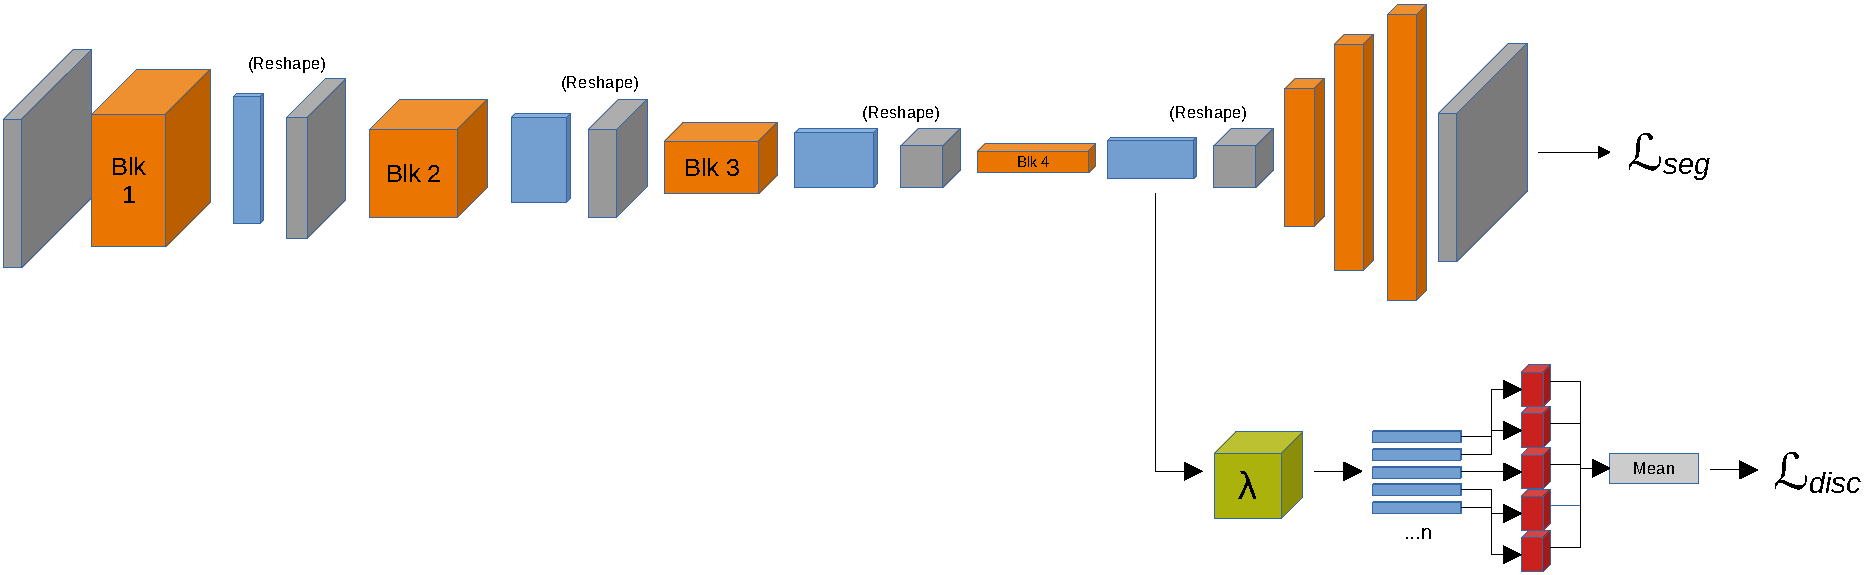
\includegraphics[width=0.8\textwidth]{res/discriminator-diagrams/patch.pdf}
    \caption{Architecture of patch-wise discriminator.}
    \label{fig:das-discriminators-patch-wise}
\end{figure*}

\subsubsection{Patch-wise output discriminator}
Applying the same principle as with the patch-wise discriminator, we follow an approach similar to \cite{hoffman_fcns_2016} by producing a convolutional output-level discriminator that takes in images in patches. \cite{hoffman_fcns_2016} operates at the feature level with patch size equal to the receptive field of the model. Since patch-level feature discrimination is already done by the patch-wise discriminator, we perform it at the output level. As "receptive field" does not exist in transformers as it does in CNNs, we make the patch size the output resolution divided by the resolution at the deepest level of SegFormer, which roughly corresponds to one prediction per patch encoding.

\bigbreak
\begin{figure*}[h]
    \centering
    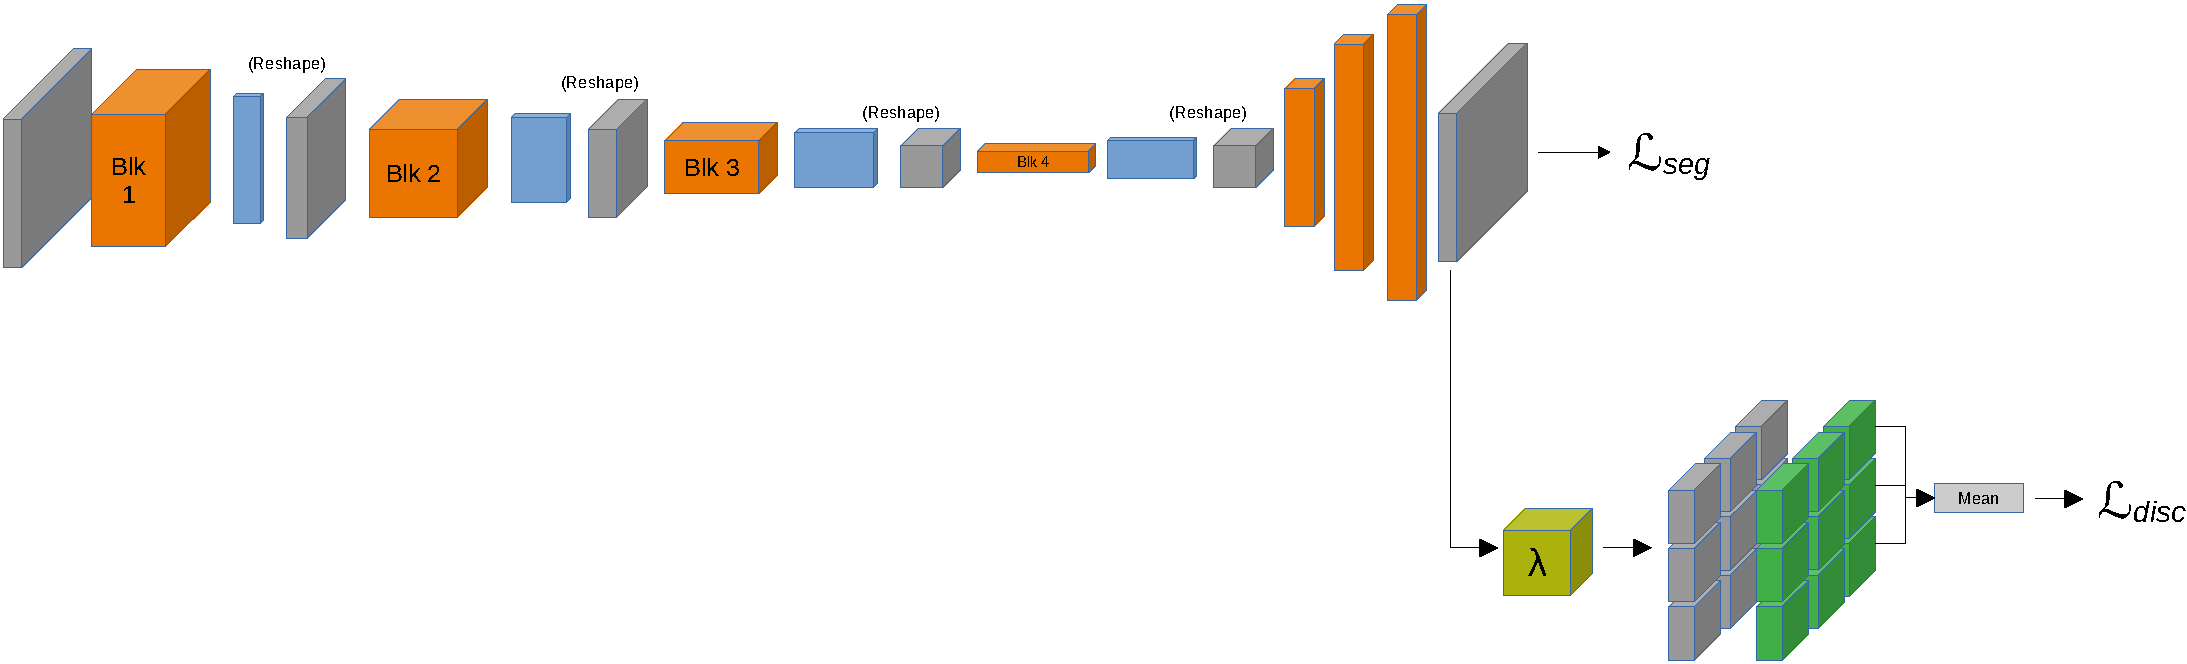
\includegraphics[width=0.8\textwidth]{res/discriminator-diagrams/patch-convolutional-output.pdf}
    \caption{Architecture of patch-wise convolutional output-level discriminator.}
    \label{fig:das-discriminators-patch-conv-output}
\end{figure*}

\subsubsection{Multi level discriminator ensemble}
As many approaches establish \cite{hoffman_fcns_2016} \cite{bermudez-chacon_domain-adaptive_2018}, the complexity of the semantic segmentation task means aligning features at a single point is often insufficient. Therefore, we deploy multiple combinations of different discriminators at multiple levels throughout the model. This includes multiple feature-level discriminators and a feature-level and output-level discriminator combination, similar to \cite{tsai_learning_2020}. Discriminator choices are based on the most successful configurations in previous experiments.

\subsubsection{Fine class-wise discriminator}
To combat the marginalisation of classes, we apply an approach similar to FADA \cite{wang_classes_2020}, making predictions not only on domain but also classes within the domain. This involves constructing fine domain labels from the segmentation head output to be passed to the discriminator (\autoref{fig:das-discriminators-fada}).

\bigbreak
\begin{figure*}[h]
    \centering
    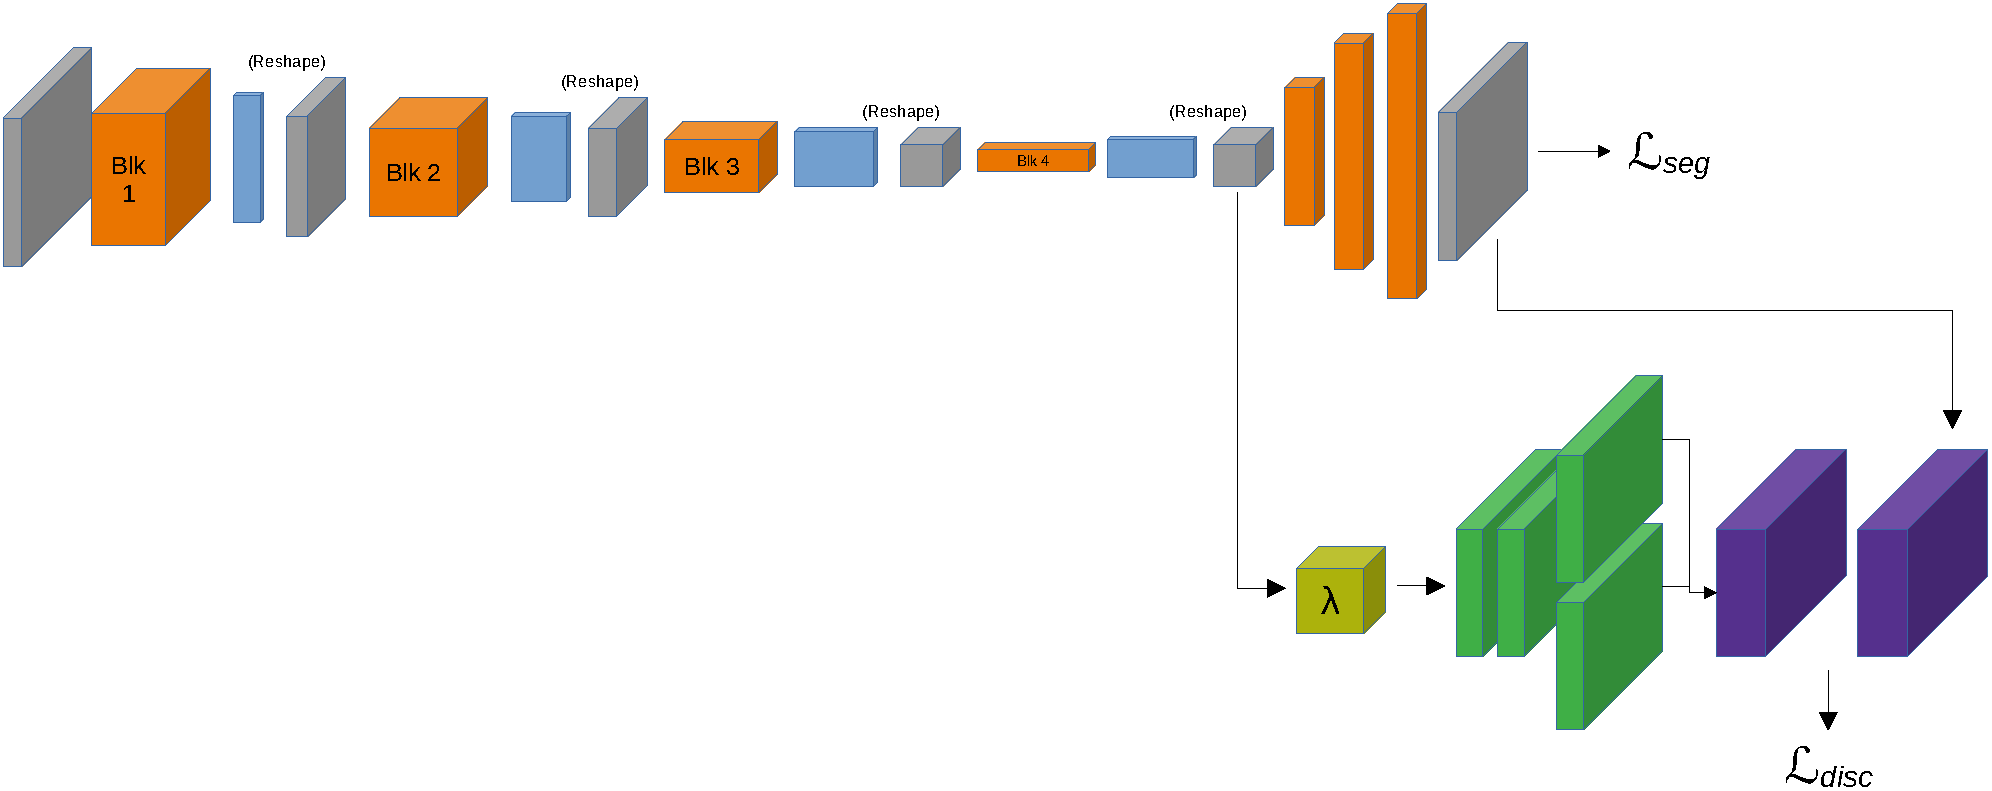
\includegraphics[width=0.8\textwidth]{res/discriminator-diagrams/fada.pdf}
    \caption{Architecture of FADA-like discriminator.}
    \label{fig:das-discriminators-fada}
\end{figure*}

\subsection{Auxiliary approaches}
A core issue identified since the inception of domain adversarial segmentation networks \cite{hoffman_fcns_2016} is the marginalisation of complex feature space caused by discriminators. While not a significant issue in simple single-class prediction tasks like classification, discriminators can encourage the model to make discriminator input features more similar at the cost of nuanced class details or distribution. For example, this could express itself in the Cityscapes dataset: As roads make up a large proportion of the training set, the model may sooner learn to make road features domain-indiscriminate compared to other features. Therefore, to fool the discriminator, it will predict road over other classes, reducing their accuracy in the training set. Several methods are explored in this work to mitigate these effects.

\subsubsection{Class distribution alignment}
Our own implementation of class distribution alignment is an extremely forward solution to the domain distribution problem. We make the assumption that the distribution between the source and target domains will be similar, and that the distribution of target dataset predicted classes should therefore also be similar. Therefore, we introduce a new loss component to source and target predictions in the similarity between the output prediction distribution and the overall distribution.

To this end, we first use pixel-counting scripts to determine the class distribution of the GTA and Cityscapes datasets (\autoref{tab:gta-dataset-distribution}), as this information was not found to be reliably available online. For the convenience of other researchers, we make the distribution publicly available \footnote{https://github.com/Moritz-Bergemann/gta5-dataset-class-distribution}. With the notable exception of the sky class, we find our intuition to be correct - in this case, the distribution of simulated and real-world data is similar. This would vary on a case-by-case basis, however.

\begin{table}[]
    \resizebox{\textwidth}{!}{%
        \begin{tabular}{|r|l|r|r|r|r|r|}
            \hline
            \multicolumn{1}{|l|}{Train Label}                                                      & Name(s)       & \multicolumn{1}{|l|}{GTA \# Pixels} & \multicolumn{1}{|l|}{\begin{tabular}[c]{@{}l@{}}GTA \\ Proportion\\ (\%)\end{tabular}} & \multicolumn{1}{|l|}{\begin{tabular}[c]{@{}l@{}}Cityscapes \# \\ Pixels\end{tabular}} & \multicolumn{1}{|l|}{\begin{tabular}[c]{@{}l@{}}Cityscapes \\ Proportion (\%)\end{tabular}} & \multicolumn{1}{|l|}{\begin{tabular}[c]{@{}l@{}}\textbf{Change} \\ \textbf{(GTA $\rightarrow$ CS)}\end{tabular}} \\ \hline
            0                                                                                      & road          & 16099193283                         & 36.14                                                                                  & 2381272463                                                                            & 36.99                                                                                       & \textbf{-0.85}                                                                                                   \\ \hline
            1                                                                                      & sidewalk      & 4155428633                          & 9.33                                                                                   & 385591016                                                                             & 5.99                                                                                        & \textbf{+3.34}                                                                                                   \\ \hline
            2                                                                                      & building      & 8478285320                          & 19.03                                                                                  & 1460671821                                                                            & 22.69                                                                                       & \textbf{-3.66}                                                                                                   \\ \hline
            3                                                                                      & wall          & 925367586                           & 2.08                                                                                   & 42931905                                                                              & 0.67                                                                                        & \textbf{+1.41}                                                                                                   \\ \hline
            4                                                                                      & fence         & 317481282                           & 0.71                                                                                   & 56014192                                                                              & 0.87                                                                                        & \textbf{-0.16}                                                                                                   \\ \hline
            5                                                                                      & pole          & 531401266                           & 1.19                                                                                   & 81333572                                                                              & 1.26                                                                                        & \textbf{-0.07}                                                                                                   \\ \hline
            6                                                                                      & traffic light & 67288808                            & 0.15                                                                                   & 13323699                                                                              & 0.21                                                                                        & \textbf{-0.06}                                                                                                   \\ \hline
            7                                                                                      & traffic sign  & 40463971                            & 0.09                                                                                   & 36631749                                                                              & 0.57                                                                                        & \textbf{-0.48}                                                                                                   \\ \hline
            8                                                                                      & vegetation    & 3810296251                          & 8.55                                                                                   & 1037416846                                                                            & 16.12                                                                                       & \textbf{-7.56}                                                                                                   \\ \hline
            9                                                                                      & terrain       & 1074861777                          & 2.41                                                                                   & 71590762                                                                              & 1.11                                                                                        & \textbf{+1.30}                                                                                                   \\ \hline
            10                                                                                     & sky           & 6784666433                          & 15.23                                                                                  & 252167629                                                                             & 3.92                                                                                        & \textbf{+11.31}                                                                                                  \\ \hline
            11                                                                                     & person        & 181828023                           & 0.41                                                                                   & 79092540                                                                              & 1.23                                                                                        & \textbf{-0.82}                                                                                                   \\ \hline
            12                                                                                     & rider         & 15321782                            & 0.03                                                                                   & 9415439                                                                               & 0.15                                                                                        & \textbf{-0.11}                                                                                                   \\ \hline
            13                                                                                     & car           & 1259269812                          & 2.83                                                                                   & 446261529                                                                             & 6.93                                                                                        & \textbf{-4.11}                                                                                                   \\ \hline
            14                                                                                     & truck         & 564950248                           & 1.27                                                                                   & 17535462                                                                              & 0.27                                                                                        & \textbf{+1.00}                                                                                                   \\ \hline
            15                                                                                     & bus           & 184638969                           & 0.41                                                                                   & 16560020                                                                              & 0.26                                                                                        & \textbf{+0.16}                                                                                                   \\ \hline
            16                                                                                     & train         & 32522117                            & 0.07                                                                                   & 13896040                                                                              & 0.22                                                                                        & \textbf{-0.14}                                                                                                   \\ \hline
            17                                                                                     & motorcycle    & 15799033                            & 0.04                                                                                   & 6174825                                                                               & 0.10                                                                                        & \textbf{-0.06}                                                                                                   \\ \hline
            18                                                                                     & bicycle       & 2718199                             & 0.01                                                                                   & 29350476                                                                              & 0.46                                                                                        & \textbf{-0.45}                                                                                                   \\ \hline
            255                                                                                    & void          & 5605086111                          & \multicolumn{1}{|l|}{-}                                                                & 850371215                                                                             & \multicolumn{1}{|l|}{-}                                                                     & \multicolumn{1}{|l|}{-}                                                                                          \\ \hline
            \multicolumn{1}{|l|}{\begin{tabular}[c]{@{}l@{}}Total \\ (Ignoring Void)\end{tabular}} & -             & 44541782793                         & 100.00                                                                                 & 6437231985                                                                            & 100.00                                                                                      & \multicolumn{1}{|l|}{}                                                                                           \\ \hline
        \end{tabular}
    }
    \caption{Class distribution of Cityscapes \cite{cordts_cityscapes_2016} vs GTA5 \cite{richter_playing_2016} datasets.}
    \label{tab:gta-dataset-distribution}
\end{table}


\subsubsection{Rare class sampling}
Another way of encouraging the model to predict rare classes is by increasing their proportion during training through oversampling of relevant images. We employ DAFormer's Rare Class Sampling (RCS) \cite{hoyer_daformer_2022}, which randomly selects a class in the target set and then selects images for the minibatch guaranteed to possess this class. The probablility of selecting each class is given by:

\begin{equation}
    P(c) = \frac{e^{(1-f_c)/T}}{\sum_{c'=1}^{C}{e^{(1-f_{c'})/T}}}
\end{equation}

Where $c$ is the class, $f_c$ is the frequency of the class, $C$ is the number of classes, and $T$ is a temperature hyperparameter, which we set to $0.01$.

\section{Experimental Results}
We use PyTorch 1.8 in an Ubuntu server with a single 2080Ti for all experiments. All experiments use a learning rate of $6 \times 10^{-5}$. All experimental results are on the Cityscapes validation dataset.


\subsection{Initial Results and Experimentation}
An interesting experiment helps demonstrate the adversarial learning approach. If the discriminator's gradient reversal layer is removed, source dataset performance will be maintained as normal, though target dataset performance will be completely destroyed, nearing 0\% mIoU. This is as the segmentation network's loss function essentially becomes $\mathcal{L}_{seg} + \mathcal{L}_{disc}$ - it is encouraged to both produce maximum performance on the source set and to make it as easy as possible for the discriminator to distinguish source and target samples, eliminating domain transfer knowledge from the model.

Initial experiments reveal a core issue with our approach. Regardless of what combinations of simple discriminators and parameters were attempted, performance on the target dataset was reduced, not increased. We initially believed this to be an issue in our experimental setup, but verified our methods using a baseline experiment. Taking advantage of the flexible domain adaptation built upon MMSegmentation, we attached a simple DCGAN-like output-level discriminator to DeepLabV3+ using ResNet-50. Though this was not an optimal setup, it should still be expected to produce some improvement based on existing works \cite{tsai_learning_2020}, and the model did improve DeepLabV3+'s performance in the GTA \textrightarrow Cityscapes task (\autoref{tab:das-baseline-experiment}). This indicates that our pipeline, while effective on existing models (and using a discriminator agnostic to feature space) improves the performance of past models but reduces the performance of SegFormer. While no specific cause could be diagnosed for this, we believe it to be an effect of transformers' baseline transferability due to self-attention \cite{dosovitskiy_image_2021} combined with the tendency for domain adversarial models to marginalise class distribution. In the case of SegFormer, the baseline model is already so effective that the improvement brought by making features domain indiscriminate is outweighed by the negative effects of marginalising the feature distribution and interfering with self-attention's input-adaptive features. Throughout the rest of this chapter, we explore how different domain adversarial approaches interact with this issue and approaches to mitigate it.

\begin{table}[]
    \resizebox{\textwidth}{!}{%
        \begin{tabular}{|l|r|r|r|}
            \hline
            Model                 & mIoU (source-only) & mIoU (with discriminator) & Relative Change \\
            \hline
            DeelabV3+ (ResNet-50) & 33.9               & 35.97                     & +2.07           \\
            \hline
            SegFormer (MiT-B3)    & 41.78              & 39.38                     & -2.40           \\
            \hline
        \end{tabular}
    }
    \caption{Baseline experiment results comparing SegFormer and DeeplabV3+. Both experiments used a simplified DCGAN-like \cite{radford_unsupervised_2016} discriminator consisting of 3 convolutional layers with 64, 128, and 2 channels respectively.}
    \label{tab:das-baseline-experiment}
\end{table}

\subsection{Adaptation factor settings}
As the adaptation factor $\lambda$ determines the extent to which the model is influenced by the discriminator, it is a key aspect of successful model performance. Therefore, we first compare a number of adaptation factor configurations. As the segmentation and discriminator model performances are expected to be low initially, many domain adversarial approaches schedule the learning rate to grow over time, typically using the following growth formula \cite{ganin_domain-adversarial_2016}:

\begin{equation}
    \lambda = \frac{2}{1 + \exp(-\gamma p)} - 1
\end{equation}

Our initial experiments ignored this factor and set $\lambda$ to a large value ($>1$), destroying model performance. To compare $\lambda$ values, we use a simple linear discriminator on the final encoder feature block output.

Many papers in the semantic segmentation space do not use gradient reversal, but scale the discriminator loss impact on the segmentation network by factors around $0.0001$-$0.001$ for a similar effect. Our results reinforce these values. While no discriminator still performs the strongest, small adaptation factors are very close. Using $\lambda$ growth with large values like 1 still achieves strong results, but strongest are achieved with small learning rate values of 0.01 (with growth) and 0.001 (without growth). Surprisingly, using growth did not achieve the strongest results, which may be as the growth becomes too large near the end of training. We initially considered (since performing source-only training performs best) that the smallest adaptation factor would perform best by minimally interfering with source-only training, but the poor performance of $\lambda = 0.0001$ indicates influences that are too small can degrade performance further.

\begin{table}[]
    \centering
    \begin{tabular}{|r|l|r|l|}
        \hline
        \multicolumn{1}{|l|}{Max AF} & Use Growth & \multicolumn{1}{l|}{\ \ \ \ \ \ \ mIoU} & Notes       \\ \hline
        \multicolumn{1}{|l|}{-}      & -          & \textbf{41.78}                          & Source-Only \\ \hline
        0.001                        & No         & \textbf{40.11}                          &             \\ \hline
        0.0001                       & No         & 35.53                                   &             \\ \hline
        1                            & Yes        & 30.53                                   &             \\ \hline
        0.1                          & Yes        & 39.46                                   &             \\ \hline
        0.01                         & Yes        & 39.28                                   &             \\ \hline
    \end{tabular}
    \caption{Results of using different adaptation factor ($\lambda$) for GTA \textrightarrow CS}
\end{table}

\subsection{Comparison of DAS architectures}

We assess all discriminator architectures using the same adaptation factor growth settings. Specific configuration information can be seen in \autoref{tab:das-disc-configurations}.

\subsubsection{Individual Discriminators}
Unfortunately, all tested discriminators were unable to surpass the baseline performance of SegFormer-MiTB3. Some discriminators had significantly less negative effects than others. The patch-wise discriminators performed strongest, which may be as its focus on individual patches minimally marginalises the overall distribution. However, the unique patch-wise discriminator only performed very slightly better than the patch-wise using the same weights for all patches, indicating avoiding marginalisation at this level is not relevant to domain transfer. Linear discriminators also performed strongly, suggesting discriminators aligned with the structure of the remaining model may be beneficial. The patch-wise discriminator mirrors the SegFormer blocks, while the linear discriminator is modelled after SegFormer's decoder. Surprisingly, the convolutional patch-wise discriminator performed extremely poorly, unlike its feature patch-wise counterpart. Investigation found no implementation issues, and integrated evaluation metrics show the discriminator is predicting accurately (~80\% accuracy).

\begin{table}[h]
    \centering
    \begin{tabular}{|l|l|r|}
        \hline
        Discriminator     & Position   & \multicolumn{1}{l|}{mIoU (\%)} \\ \hline
        Linear            & Last Feat. & 40.11                          \\ \hline
        Convolutional     & Last Feat. & 38.95                          \\ \hline
        DCGAN             & Output     & 39.65                          \\ \hline
        Patch-Wise        & Last Feat. & 40.41                          \\ \hline
        Unique Patch-Wise & Last Feat. & 40.4                           \\ \hline
        Conv Patch-wise   & Output     & 6.88                           \\ \hline
    \end{tabular}
    \caption{Baseline performance of DAS discriminators. All use $\lambda=0.001$ without growth.}
\end{table}

\subsubsection{Ensemble methods}
Our ensembles consisted of a feature-level ensemble (using patch discriminators) and a feature-output level ensemble, using patch and DCGAN-like discriminators. Following \cite{tsai_learning_2020}, we deploy discriminators in the final 2 layers of the model. For memory-related reasons, the DCGAN discriminator was reduced in size.

\begin{table}[h]
    \centering
    \begin{tabular}{|l|r|}
        \hline
        Ensemble                      & \multicolumn{1}{l|}{mIoU} \\ \hline
        2 feature-level patch         & 39.32                     \\ \hline
        2 feature-level patch + DCGAN & 34.43                     \\ \hline
    \end{tabular}
    \caption{Results of ensemble discriminators on DAS.}
\end{table}

Surprisingly, ensemble methods did not outperform their individual counterparts, and in fact performed worse. We expected the ensembles to aid in the alignment of the overall feature space as in previous approaches \cite{hoffman_fcns_2016} \cite{chen_learning_2017}, but found this not to be the case. This may be as the issue of class-level alignment or dynamic feature marginalisation is present at a deeper level.

\begin{table}[]
    \centering
    \resizebox{!}{0.35\paperheight}{%
        \begin{tabular}{|l|l|}
            \hline
            \textbf{Discriminator}                 & \textbf{Specific layout}                                                                                                                                                                                                                                                                                                                                                                                                                                           \\ \hline
            Linear                                 & \begin{tabular}[c]{@{}l@{}}Linear Layer ($F$ input to 768 output channels)\\ ReLU\\ LInear Layer (768 input to 768 output channels)\\ ReLU\\ Pointwise Convolutional Layer (768 input to 2 output channels)\\ Global average pooling\end{tabular}                                                                                                                                                                                                                  \\ \hline
            Convolutional                          & \begin{tabular}[c]{@{}l@{}}Convolutional Layer ($F$ input to 32 output channels)\\ Convolutional Layer (32 input to 2 output channels)\\ Global average pooling\end{tabular}                                                                                                                                                                                                                                                                                       \\ \hline
            DCGAN \cite{radford_unsupervised_2016} & \begin{tabular}[c]{@{}l@{}}Conv. Layer ($C$ input channels, 64 output channels, stride 2)\\ Leaky ReLU\\ Conv. Layer (64 input channels, 128 output channels, stride 2)\\ Leaky ReLU\\ Conv. Layer (128 input channels, 256 output channels, stride 2)\\ Leaky ReLU\\ Conv. Layer (256 input channels, 512 output channels, stride 2)\\ Leaky ReLU\\ Conv. Layer (512 input channels, 2 output channels, stride 2)\\ Global average pooling\\ Sigmoid\end{tabular} \\ \hline
            patch-wise                             & \begin{tabular}[c]{@{}l@{}}256 patches:\\ Linear layer (512 input channels, 512 // 4 = 128 output channels)\\ ReLU\\ Linear layer (128 input channels, 128 output channels)\\ ReLU\\ Linear layer (128 input channels, 2 output channels)\\ Global average pooling\\ Sigmoid\end{tabular}                                                                                                                                                                          \\ \hline
            Unique patch-wise                      & Same as patch-wise                                                                                                                                                                                                                                                                                                                                                                                                                                                 \\ \hline
            Conv patch-wise                        & \begin{tabular}[c]{@{}l@{}}16 * 16 = 256 patches\\ Conv. Layer ($C$ input channels, 32 output channels, stride 1)\\ Leaky ReLU\\ Conv. Layer (32 input channels, 64 output channels, stride 1)\\ Leaky ReLU\\ Conv. Layer (64 input channels, 2 output channels, stride 1)\\ Global average pooling\\ Sigmoid\end{tabular}                                                                                                                                         \\ \hline
            FADA \cite{wang_classes_2020}          & \begin{tabular}[c]{@{}l@{}}Conv. Layer ($F$ input channels, 512 output channels, stride 1)\\ Leaky ReLU\\ Conv. Layer (512 input channels, 256 output channels, stride 1)\\ Leaky ReLU\\ 2 $\times$ Conv. Layer (256 input channels, $C$ output channels, stride 1)\\ Concatenate previous 2 channels\end{tabular}                                                                                                                                                 \\ \hline
        \end{tabular}
    }
    \caption{Specific configuration of DAS discriminators. $C$ denotes number of classes, $F$ denotes feature depth.}
    \label{tab:das-disc-configurations}
\end{table}

\subsection{Auxiliary approaches}
We keep the loss factor for class distribution loss large (1.0) as the loss produced by the function itself is small. Due to memory restrictions, we were forced to use the simpler DCGAN disc instead of patch-wise discriminators for this stage.

\begin{figure}[h]
    \centering
    \begin{tabular}{|l|l|r|}
        \hline
        Auxiliary Method            & Discriminator & \multicolumn{1}{l|}{mIoU} \\ \hline
        RCS                         & DCGAN         & \textbf{44.76}            \\ \hline
        Class distribution matching & DCGAN         & 39.4                      \\ \hline
        Fine class matching         & DCGAN         & 37.22                     \\ \hline
        Source-Only                 & -             & 41.78                     \\ \hline
    \end{tabular}
    \caption{Results of auxiliary approaches on DAS. Adding RCS improves performance over baseline.}
\end{figure}

Distribution alignment approaches finally allowed us to improve over baseline performance. The addition of RCS increased mIoU to 44.76\%, over the baseline 41.78\%, and qualitative results show visible improvement (\autoref{fig:das-qualitative}). These results prove that it is possible to SegFormer over source-only performance using adversarial discriminators, and that at least part of the issue is related to class marginalisation and can be addressed through oversampling of rare classes. Disappointingly, neither FADA nor class distribution matching were able to mirror these results. Class-wise performance analysis showed that, while improving performance on baseline classes, these approaches reduced performance on common classes and thus overall mIoU.

\begin{figure}[]
    % \resizebox{\textwidth}{!}{%
    \centering
    \begin{tabular}{llll}
        Source Image                                                                       & Ground Truth                                                                        \\
        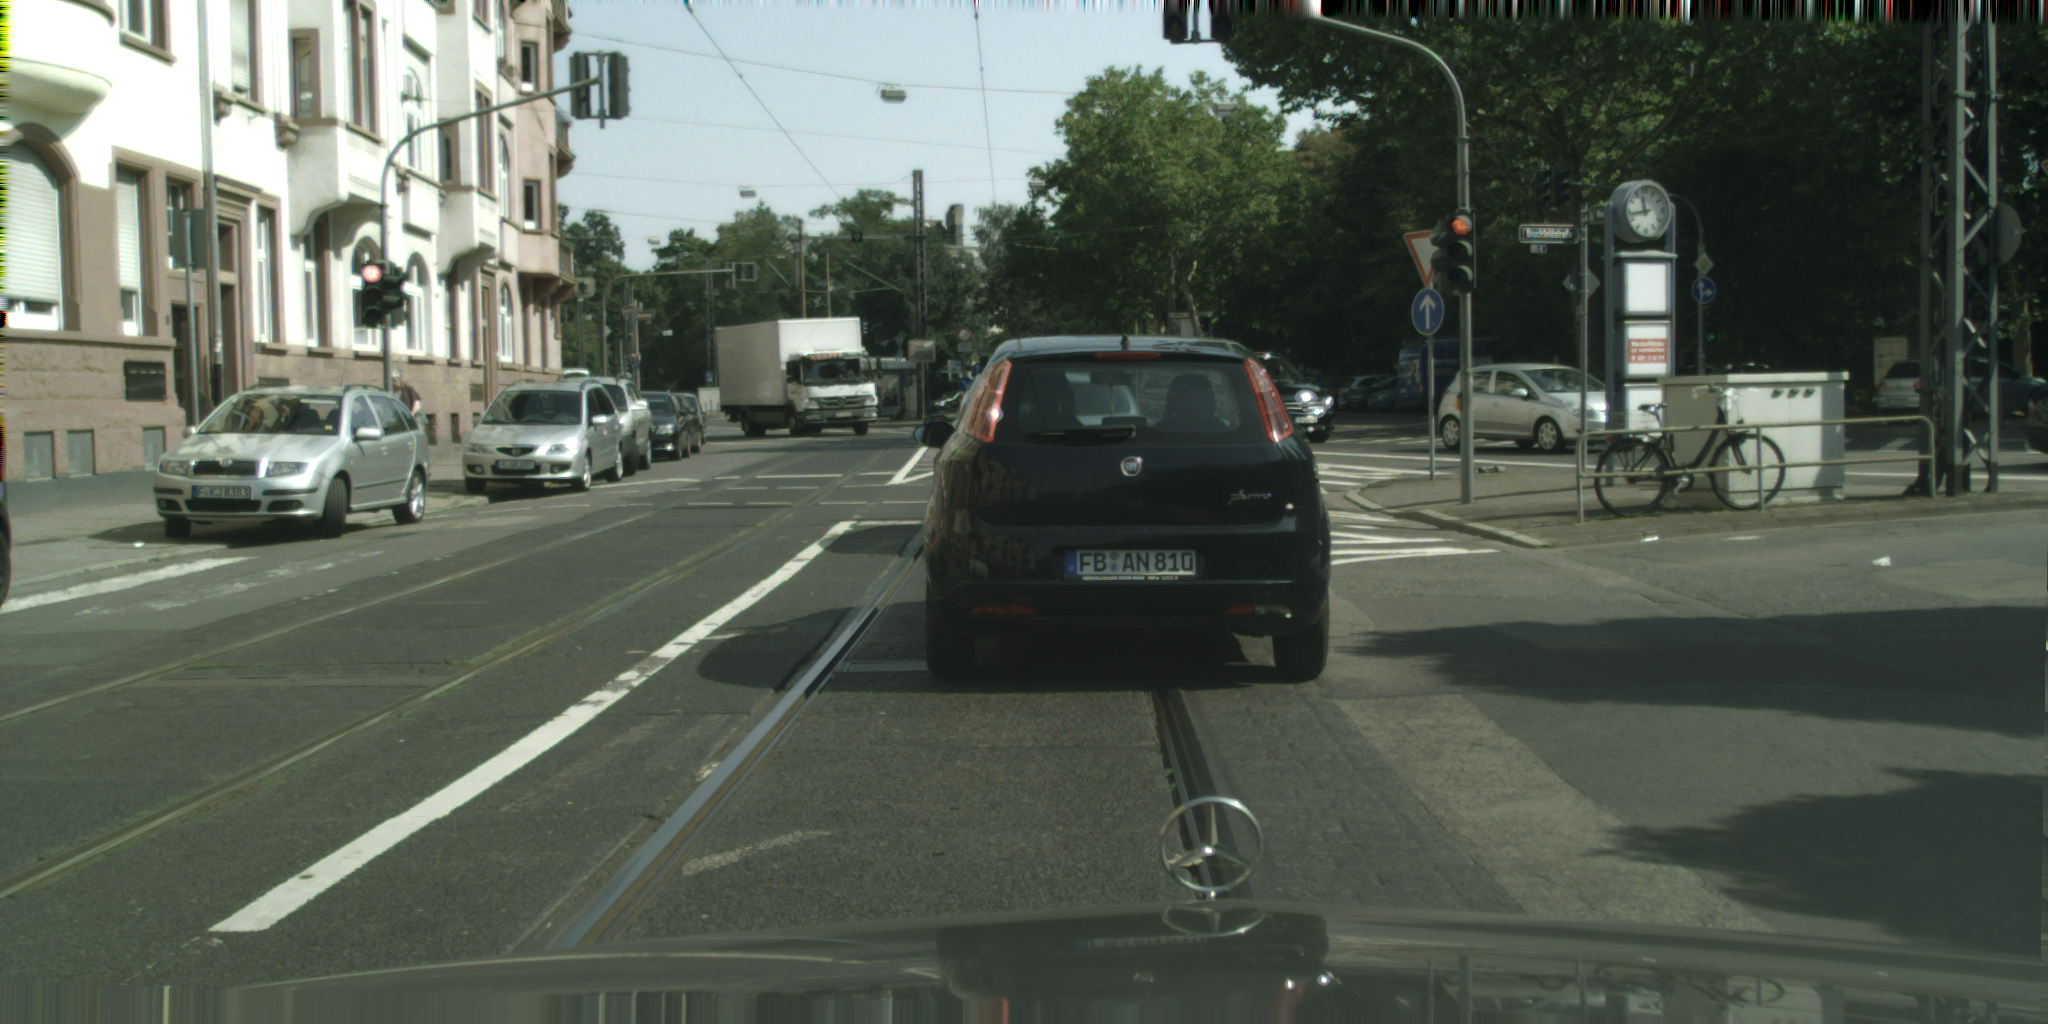
\includegraphics[width=.4\linewidth,valign=m]{res/das-qualitative/image.png}       & 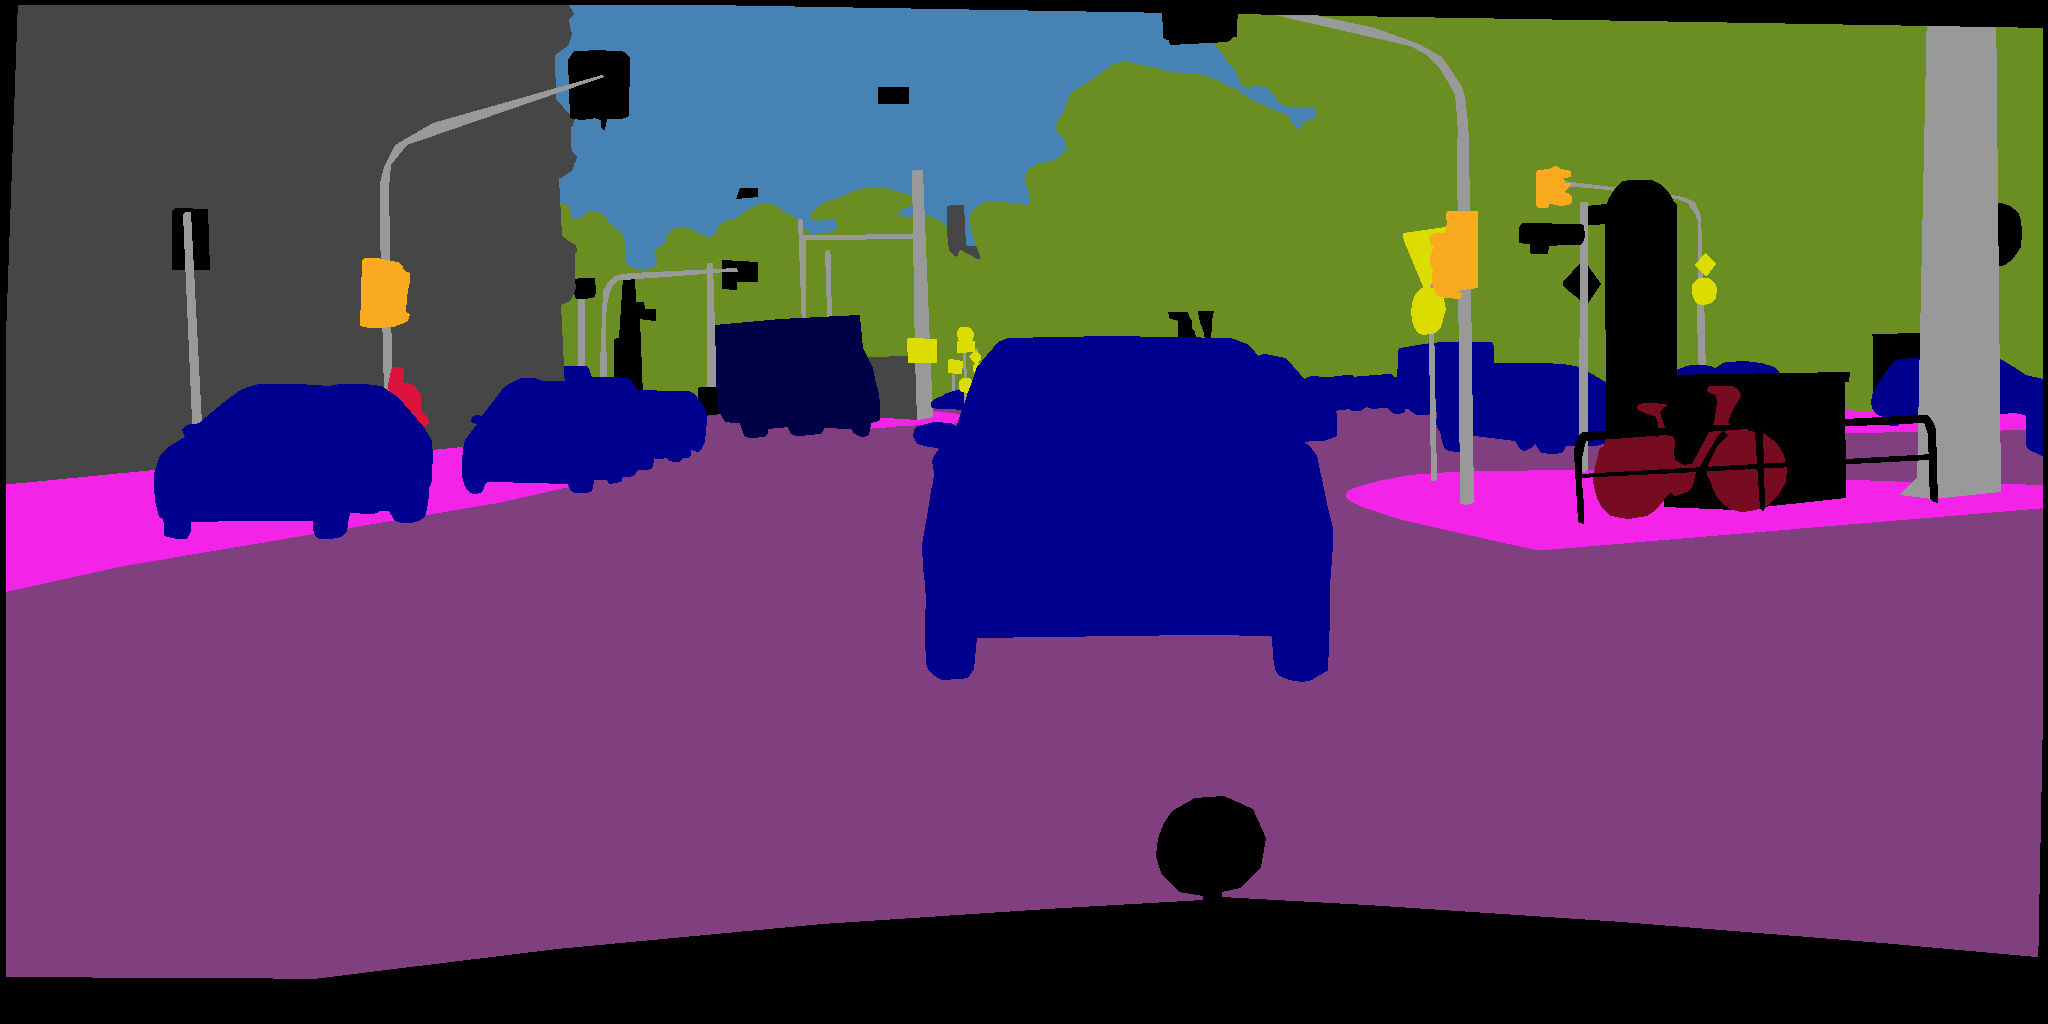
\includegraphics[width=.4\linewidth,valign=m]{res/das-qualitative/ground-truth.png} \\
        Source-Only                                                                        & DCGAN + RCS                                                                         \\
        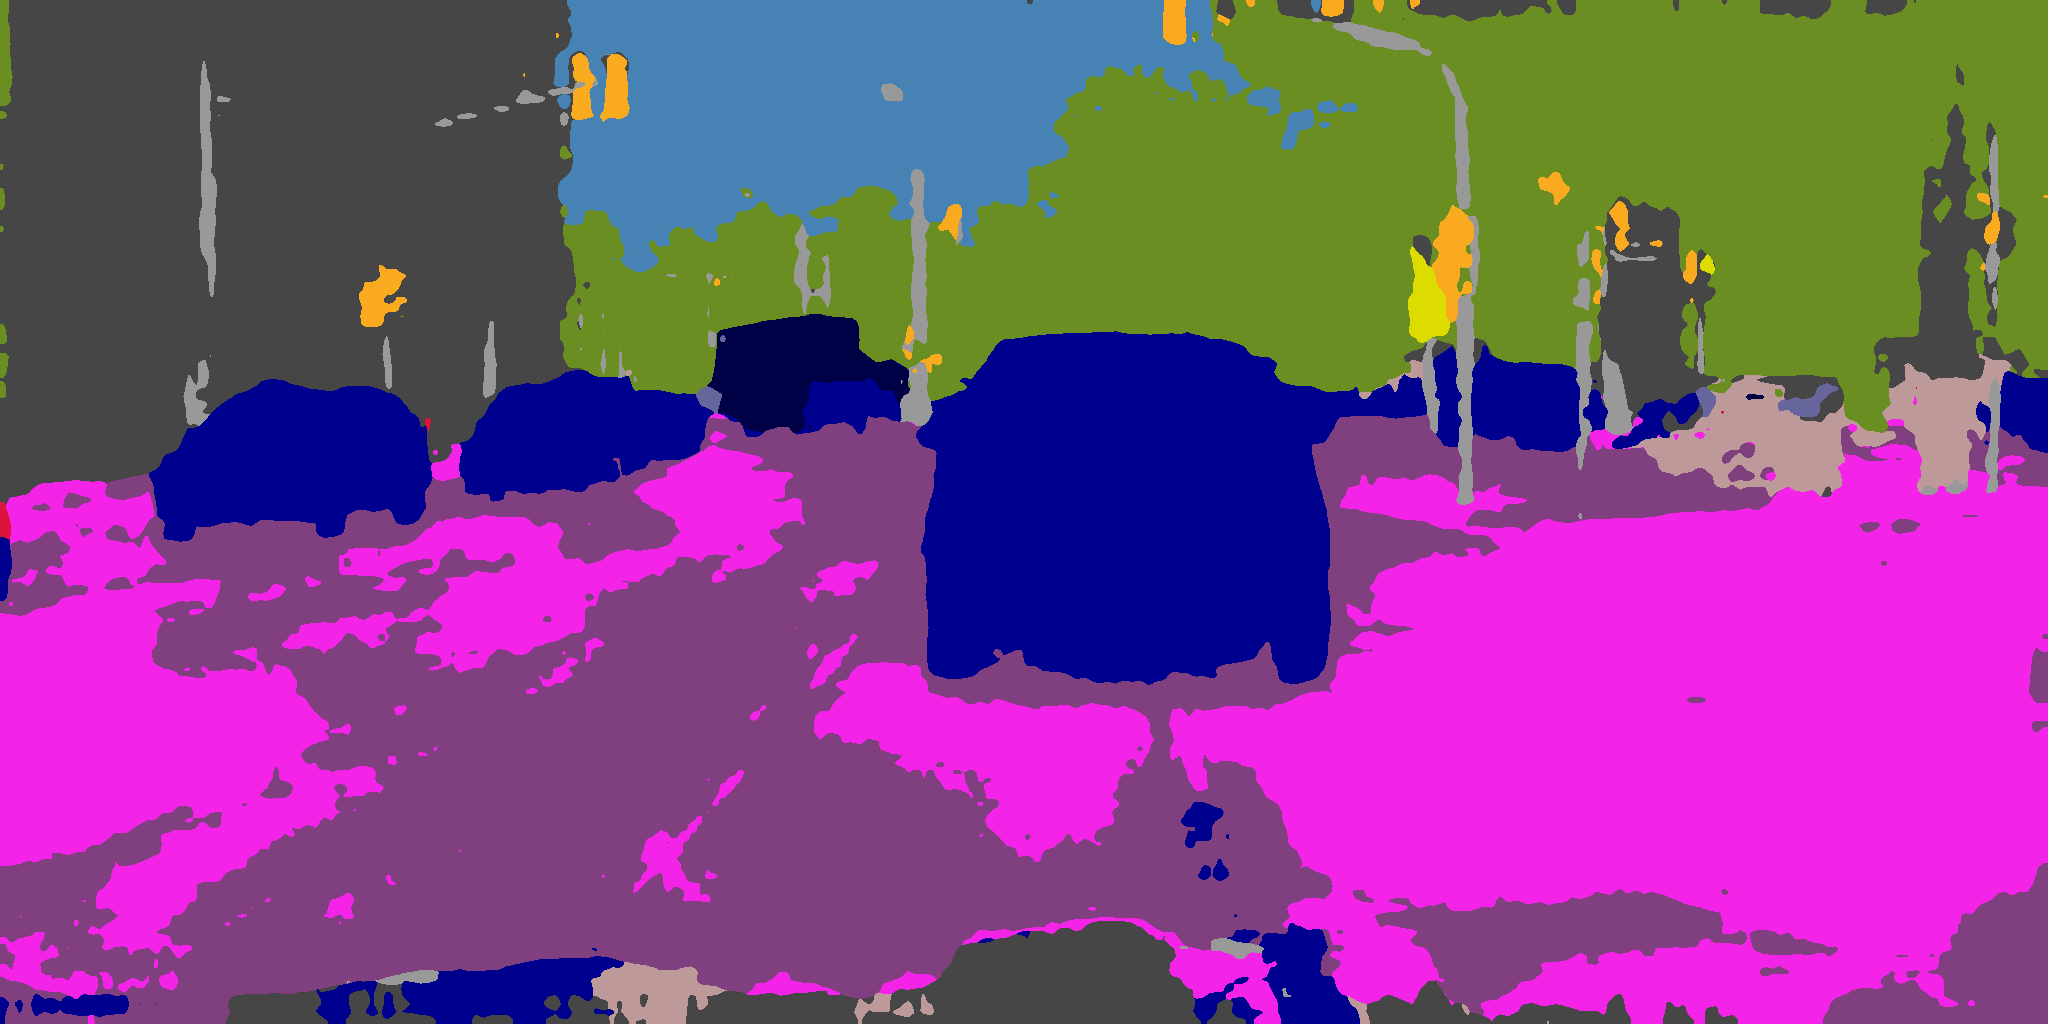
\includegraphics[width=.4\linewidth,valign=m]{res/das-qualitative/source-only.png} & 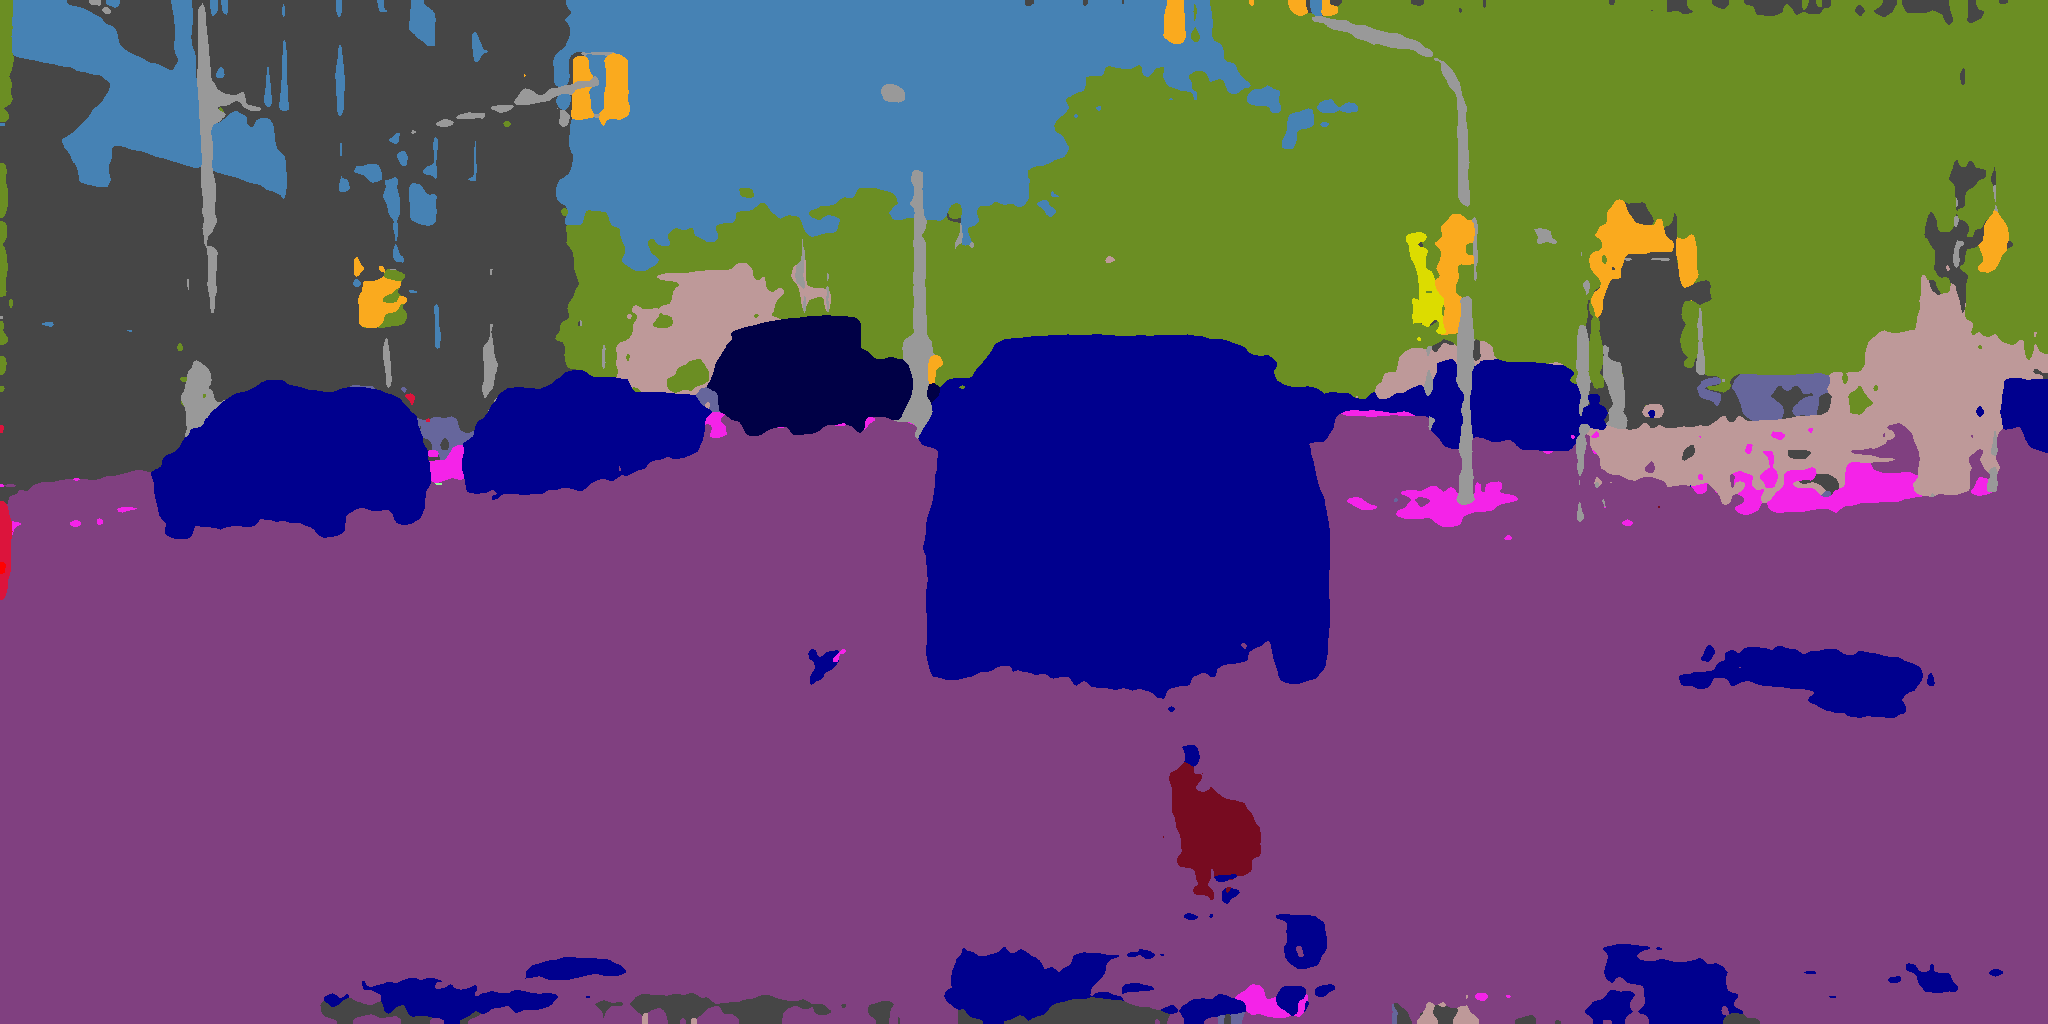
\includegraphics[width=.4\linewidth,valign=m]{res/das-qualitative/dcgan-rcs.png}    \\
    \end{tabular}
    \caption{Comparison of DCGAN + RCS DAS against source-only training.}
    \label{fig:das-qualitative}
\end{figure}

\subsection{General comments}
\subsubsection{Efficiency}
Compared to DAFormer, significantly less work is done during most DAS training approaches. Experiment duration is typically significantly shorter - DAFormer MiT-B3 experiments take around 12 hours on a 2080Ti GPU, while many DAS experiments require less than 6 hours. However, this comes at the cost of memory efficiency during training. While DAFormer is capable of running MitB5 training on a 12GB 2080Ti GPU, DAS is only capable of running all experiments using the smaller MiTB3 architecture. The increased memory cost could be somewhat mitigated by avoiding using gradient reversal and instead performing model inferences separately, but this would increase inference time and code complexity.

\section{Conclusion}
The complexity of semantic segmentation models continues to grow, and difficulty in applying a technique that simplifies model features in this chapter demonstrates this. We believe that the inherent domain adaptivity and ability to dynamically scale weights of SegFormer is only hindered by the distribution marginalisation brought by an adversarial discriminator, thus producing the worse-than-baseline results we observe.

We still demonstrate that, with the correct parameters, it is possible to improve performance over baseline with DAS, and we are confident more significant improvements are possible. However, our results are not as promising as those achieved using DAFormer's Self-Training.

\begin{table}[h]
    \centering
    \begin{tabular}{|l|l|}
        \hline
        Approach & mIoU (\%)     \\ \hline
        Baseline & 41.78         \\ \hline
        DAS      & 44.76         \\ \hline
        DAFormer \cite{hoyer_daformer_2022} & \textbf{50.8} \\ \hline
    \end{tabular}
    \caption{Comparison of best results achieved using UDA approaches on the Cityscapes dataset. All approaches use MiT-B3 as the backbone.}
\end{table}

Though disappointing, we believe the comprehensive results provided are still valuable. We demonstrate that, though there are significant and previously unseen issues, it is possible to achieve above-baseline performance with a carefully implemented strategy. In addition, the creation of an adaptive framework for domain adversarial semantic segmentation (though still in need of improvements and documentation) provides its own value, and we hope it will provide a framework that others will be able to build upon.

\section{Future work}
\begin{itemize}
    \item \textbf{Further datasets}: Due to time and resource constraints, only the common GTA \textrightarrow Cityscapes domain adaptation task was assessed in this chapter. Assessment of other datasets (e.g. Synthia \textrightarrow Cityscapes, Cityscapes \textrightarrow Cross-city) should be performed for more comprehensive results.
    \item \textbf{Patch-wise feature encouragement}: ViT's advanced method involved a discirminator that re-weighted feature patches based on their transferability. This was not implemented due to its complexity, but could aid in providing a more dynamic way of encouraging indiscriminate features.
    \item \textbf{Patch-wise class predictions} - It may be promising to combine the class-level predictions of FADA \cite{wang_classes_2020} with the patch-wise discrimination approach of TVT \cite{yang_tvt_2021}. As the latter discusses, patches often represent class-level or global feature-level information. Therefore, enocuraging patches to learn domain-indiscriminate encodings while maintaining class features may allow adversarial approaches to overcome class marginalisation. However, this approach would require a means of labelling source and target patches with class information that we could not identify.
    \item \textbf{Further regularisation techniques} - Final results indicate specific auxiliary and regularisation methods are necessary to improve performance. Approaches like ImageNet thing-class feature distance \cite{hoyer_daformer_2022} could be used to further regularise the model in attempts to reduce performance drop.
\end{itemize}

% ----------------------------------------------------------------
% Efficient Domain Adaptation with Lightweight Transformers via Pseudo-Teacher Training
% ----------------------------------------------------------------

\chapter{Efficient Domain Adaptation with Lightweight Transformers via Pseudo-Teacher Training}

Little research has been published exploring the usage of efficient neural networks for domain adaptation, especially in the segmentation space. Therefore, we explore in this chapter the domain-transferability of modern lightweight semantic segmentation networks, and propose a novel domain adaptation strategy using an autolabelling-like approach we denote pseudo-teacher learning. Using this approach, we achieve an mIoU of 61.18 on the Cityscapes dataset on a model orders of magnitude smaller and more efficient than SegFormer-B5 without using any Cityscapes labels.

\section{Background}

\subsection{Efficient Transformers for Semantic Segmentation}

While the power of large vision transformers such as ViT and SegFormer trained on larger datasets is established, these properties do not properly present themselves in highly resource-constrained contexts, where the direct inductive biases of CNNs appear to win out. For instance, \cite{mehta_mobilevit_2022} identified a version of DEiT \cite{touvron_training_2021} with only around 6 million parameters, is outperformed by the traditional CNN-based MobileNetV3 \cite{howard_searching_2019}. Therefore, recent attempts have been made to produce lightweight transformer-based computer vision models, typically by combining the efficiency and inductive biases of CNNs with the strong global learning capability of transformers.

MobileViT \cite{mehta_mobilevit_2022} is an early popular approach, which introduces CNN-like inductive biases into transformer vision models to achieve lightweight inference. MobileViT, similar to SegFormer \cite{xie_segformer_2021}, has each block's input and output be in the form of a $\mathbb{R}^{H \times W \times C}$ tensor (where $H$ is height, $W$ is width, and $C$ is channels). However, instead of performing patch embedding, MobileViT blocks first use pointwise convolutions to transform input into a high-dimensional space $\mathbb{R}^{H \times W \times d}, d > C$, then unfold it into a $\mathbb{R}^{P \times N \times d}$ tensor, (where $P$ is product of patch dimensions $h \times w$ and $N$ is the patch number). Attention is then applied along individual pixels of each patch block (\autoref{fig:mobilevit_block}) before refolding to $\mathbb{R}^{H \times W \times D}$. This process of unfolding, folding, and processing, mirrors the same process that occurs during standard convolutions \cite{contributors_unfold_nodate}, transferring over the inductive biases of the operation while applying global receptive field. MobileViT outperforms may state-of-the-art CNNs and transformer networks while possessing few parameters, using DeeplabV3's ASPP head \cite{chen_rethinking_2017} for segmentation output. It was also found to improve generalisability, the ability to perform on unseen datasets, compared to similarly-scaled transformer models.

\begin{figure}[t!]
    \centering
    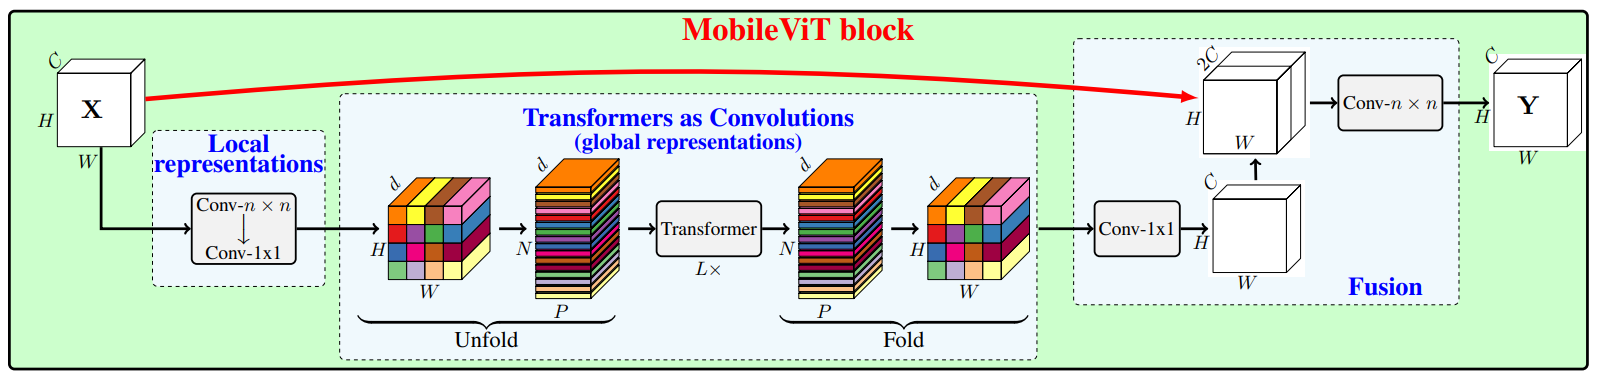
\includegraphics[width=\textwidth]{res/mobilevit-block.png}
    \caption{Architecture of a MobileViT block \cite{mehta_mobilevit_2022}. Features are input in CNN-like $H \times W \times C$ format, unfolded into a transformer input sequence, then re-folded into before being output.}
    \label{fig:mobilevit_block}
\end{figure}

Other approaches seeking efficiency combine CNNs and transformers more directly. Mobile-Former \cite{chen_mobile-former_2022} runs MobileNet and transformer blocks in parallel to achieve performance and efficiency gains over MobileNetV3, though at a still high number of FLOPs and parameters. More recently, TopFormer \cite{zhang_topformer_2022} focuses specifically on fast transformer based segmentation by using a feature pyramid-like design. First, MobileNet blocks are used to build a multiscale feature pyramid to reduce input dimension (down to $\frac{1}{64}$ of target size). All block output tokens are then average pooled to the size of the smallest and concatenated. After patch embedding, these tokens are passed through a standard vision transformer. The tokens are then reshaped, de-concatenated, and upsampled before being combined with their original counterparts. The final tokens are then combined in a convolution-based gradual upsampling process, similar to U-Net \cite{ronneberger_u-net_2015} and approaches discussed in chapter 2. The benefit of this approach is tow-fold: CNN inductive biases are applied during downsampling and upsampling and the global receptive field of transformers is applied at low convolutional cost due to the small input size. The transformer's attention also enables the sharing of features across resolutions. TopFormer achieves particularly strong results on the challenging ADE20K dataset, known for its complex scenery.

% "MobileNet convolutional" CHECK IF IT SHOULD BE BOTTLENECK?


\section{Baseline Experiments}
Note all experimental results in this chapter are on the Cityscapes validation dataset.

In order to explore efficient segmentation UDA, we apply existing methods to common state-of-the-art efficient segmentation networks. For our experiments, we specifically use Fast-SCNN \cite{poudel_fast-scnn_2019} as an example of an extremely lightweight CNN, and MobileViT \cite{mehta_mobilevit_2022} and TopFormer \cite{zhang_topformer_2022} as lightweight transformer models we expect to be more domain-adaptive. We also assess on the most light-weight possible versions of SegFormer and DAFormer, using the MiT-B0 backbone. Since DAFormer does not include a decoder for the MiT-B0 backbone, we follow SegFormer and produce one by halving channel depths in its decoder. For all experiments in this chapter, we use a batch size of 4 permitted by the increase in available memory. Wherever possible, learning rates and other hyperparameters follow the original papers.

We first compare source-only performance. Fast-SCNN performs poorly, indicating its lightweight, CNN-based architecture is not suitable for retaining complex domain-independent features. The lack of pre-training (as \cite{poudel_fast-scnn_2019} identify it does not improve model performance) may further extrapolate this. As expected, MobileViT and TopFormer both perform significantly more strongly, though their computing cost (FLOPs and parameters) is non-negligibly higher.

\begin{table}[]
    \resizebox{\textwidth}{!}{%
        \begin{tabular}{|l|l|r|l|r|r|r|}
            \hline
            Model                & \begin{tabular}[c]{@{}l@{}}Reported\\ Params\end{tabular} & \multicolumn{1}{l|}{\begin{tabular}[c]{@{}l@{}}Measured \\ Params (M)\end{tabular}} & \begin{tabular}[c]{@{}l@{}}Reported \\ FLOPs \\ (GFlops)\end{tabular} & \multicolumn{1}{l|}{\begin{tabular}[c]{@{}l@{}}Measured \\ FLOPs \\ (GFlops)\end{tabular}} & \multicolumn{1}{l|}{\begin{tabular}[c]{@{}l@{}}mIoU \\ (Source-Only)\end{tabular}} & \multicolumn{1}{l|}{\begin{tabular}[c]{@{}l@{}}mIoU \\ (UDA)\end{tabular}} \\ \hline
            Fast-SCNN            & 1.11M                                                     & 1.46                                                                                & -                                                                     & \textbf{0.94}                                                                              & 20.95                                                                              & \multicolumn{1}{l|}{-}                                                     \\ \hline
            Segformer(MiT-B0)    & 3.8M                                                      & 6.09                                                                                & \multicolumn{1}{r|}{8.4}                                              & 42.94                                                                                      & 26.57                                                                              & 47.55                                                                      \\ \hline
            DAFormer (MiT-B0)    & -                                                         & 4.26                                                                                & -                                                                     & 17.69                                                                                      & 28.12                                                                              & \textbf{50.56}                                                             \\ \hline
            MobileViT (Small)    & 6.4 M                                                     & 12.65                                                                               & -                                                                     & 16.93                                                                                      & 31.86                                                                              & 46.73                                                                      \\ \hline
            MobileViT (XX-Small) & -                                                         & 6.28                                                                                & -                                                                     & 7.08                                                                                       & 30.35                                                                              & 41.38                                                                      \\ \hline
            TopFormer (Base)     & 5.1M                                                      & 1.81                                                                                & \multicolumn{1}{r|}{2.7}                                              & 5.06                                                                                       & \textbf{33.32}                                                                     & 43.15                                                                      \\ \hline
            TopFormer (Tiny)     & 1.4M                                                      & \textbf{1.39}                                                                       & -                                                                     & 0.58                                                                                       & 27.78                                                                              & 36.98                                                                      \\ \hline
        \end{tabular}
    }
    \caption{Performance comparison of lightweight segmentation models on GTA \textrightarrow CS, with both source-only and self-training approaches.}
    \label{tab:lightweit-da-baseline}
\end{table}

\begin{figure}[]
    % \resizebox{\textwidth}{!}{%
    \centering
    \begin{tabular}{lll}
        Ground Truth       & 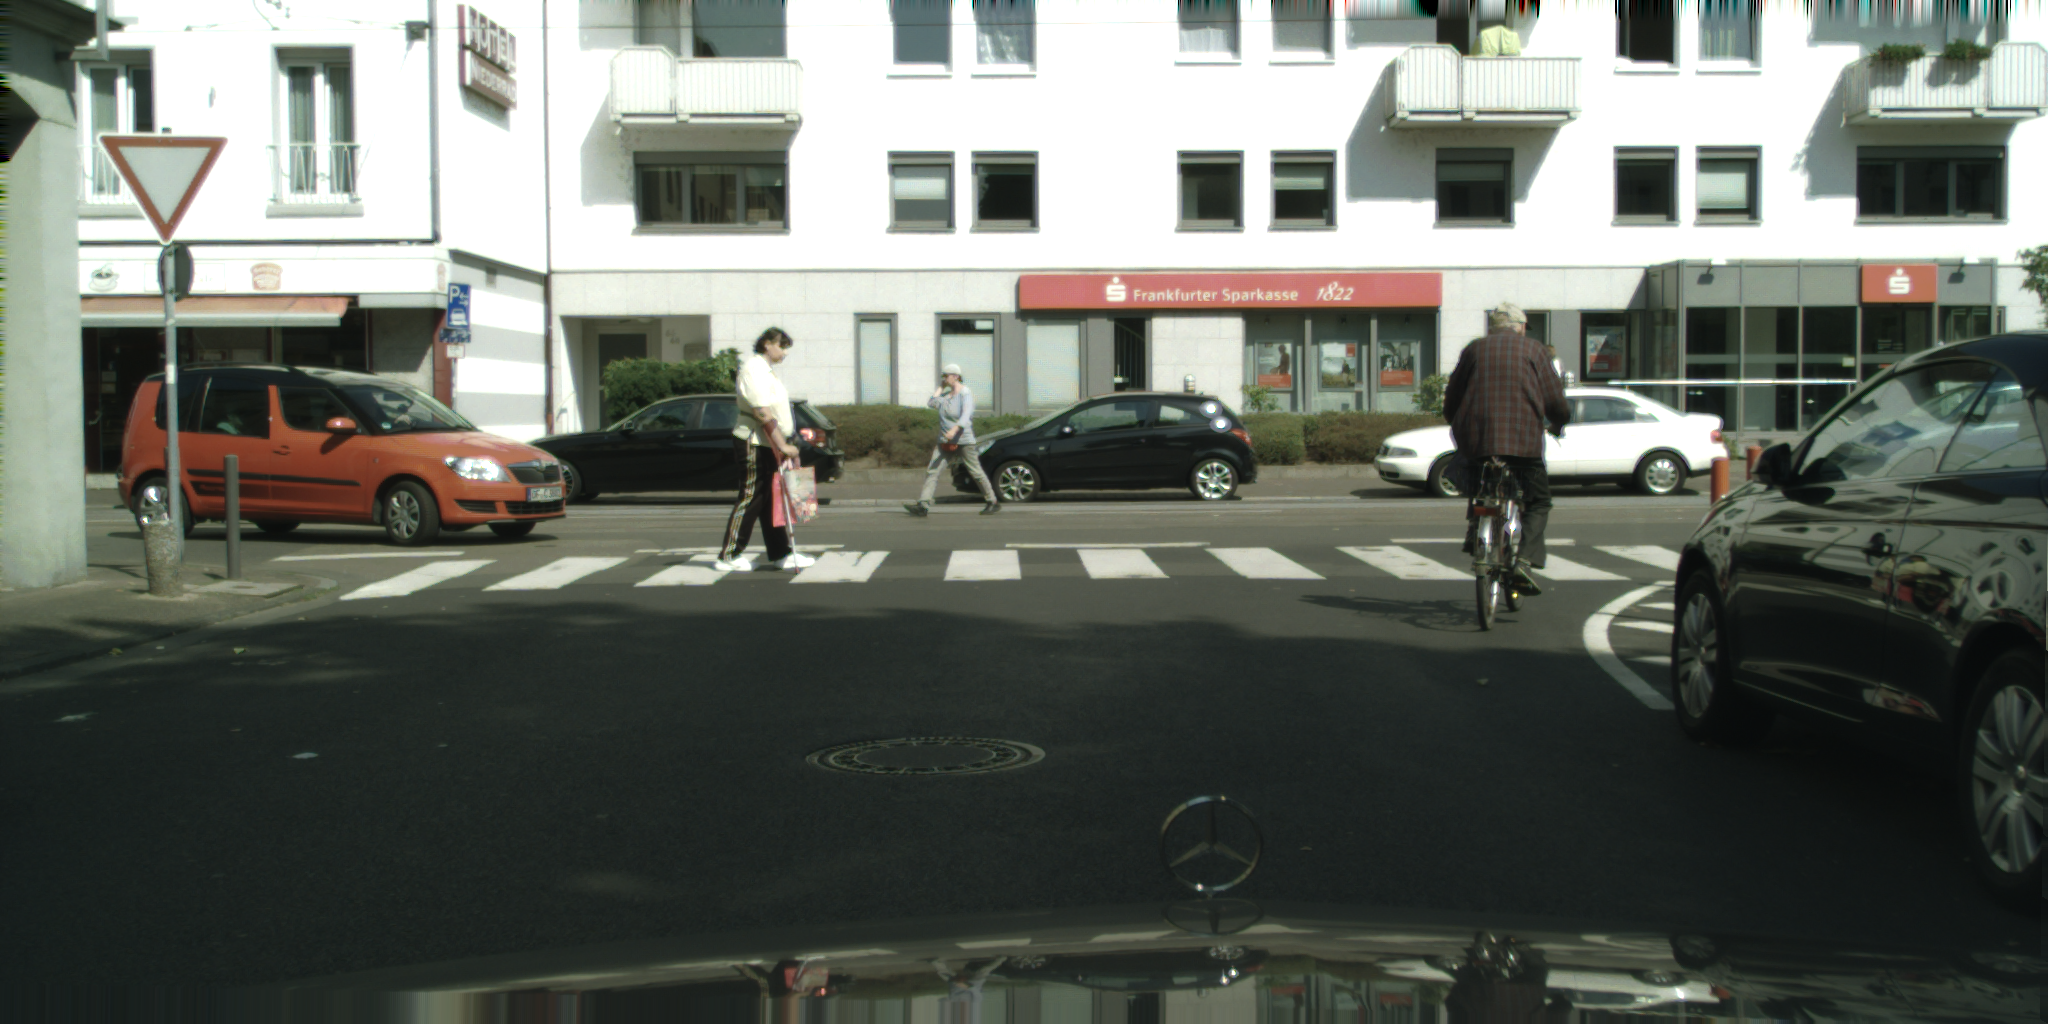
\includegraphics[width=.3\linewidth,valign=m]{res/lightweight-uda-baseline-qualitative/image.png}                         & 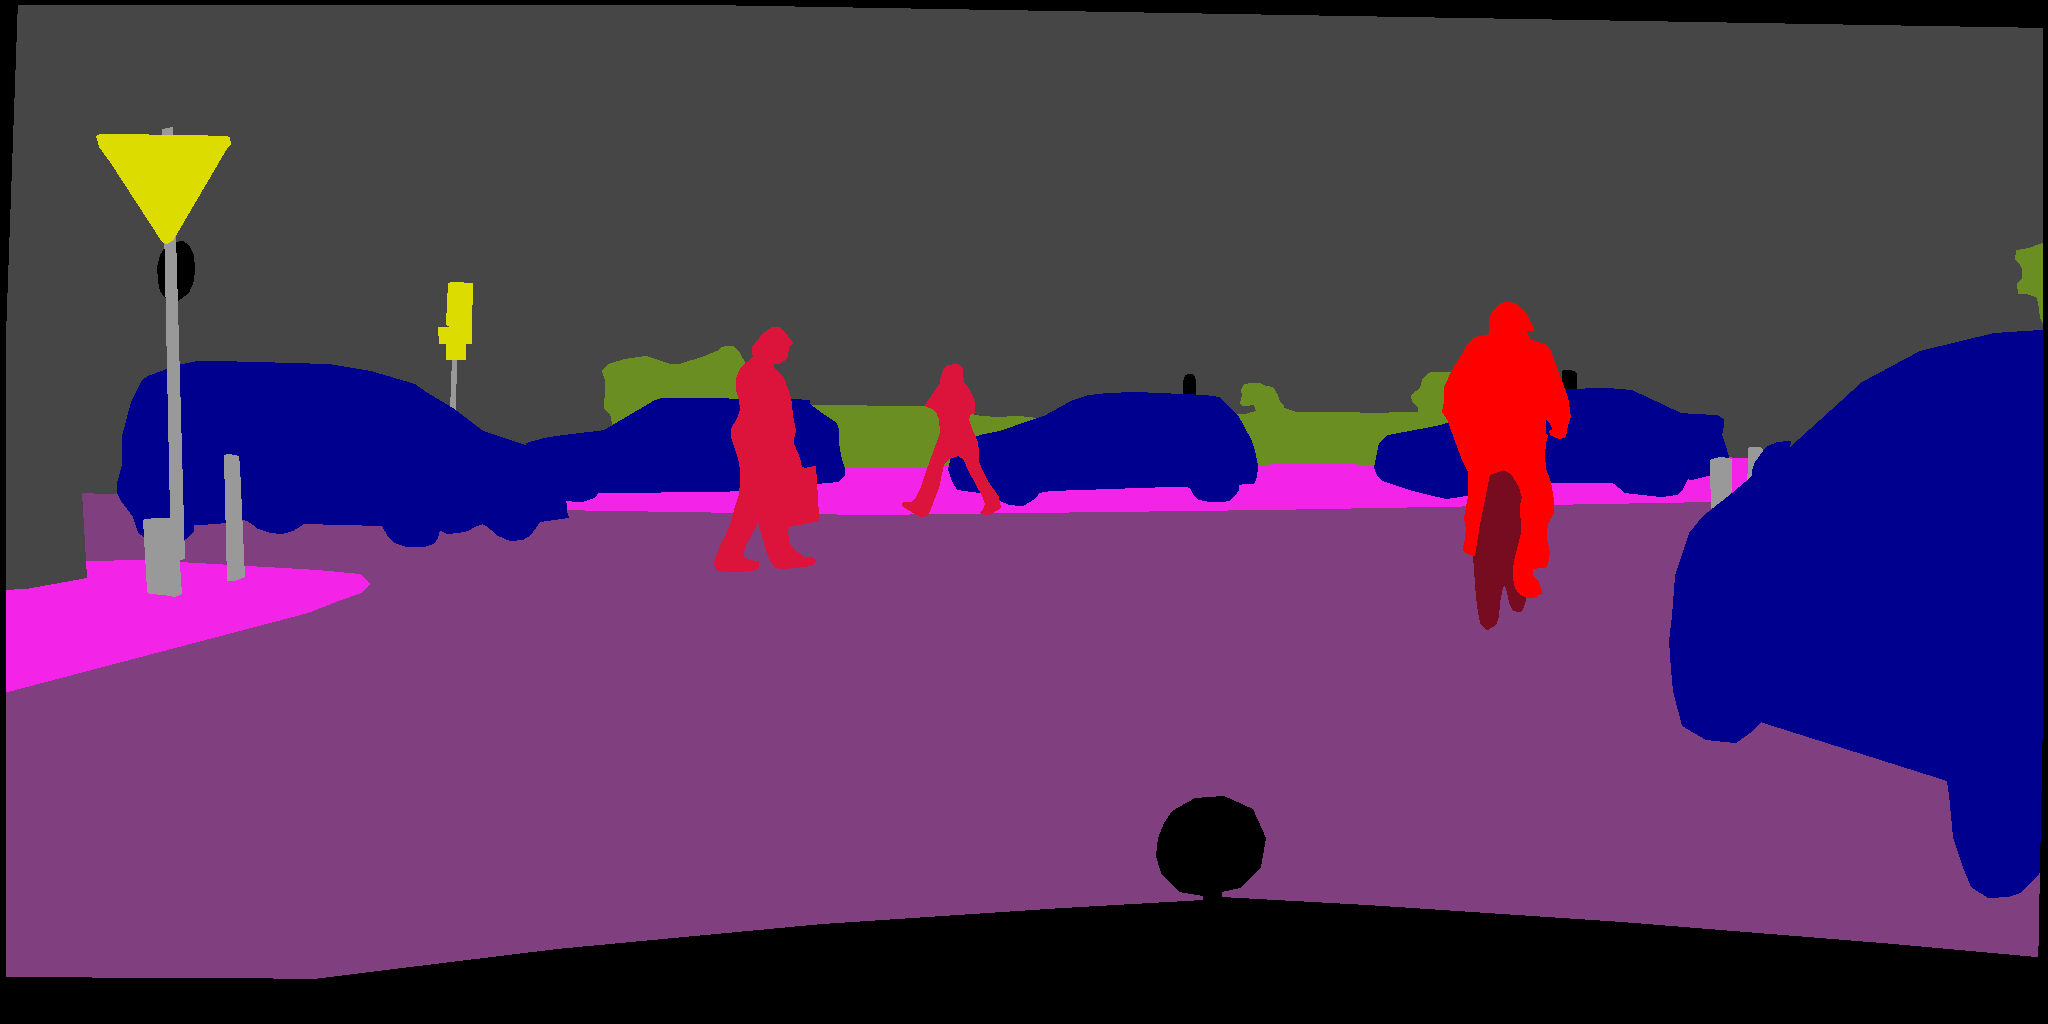
\includegraphics[width=.3\linewidth,valign=m]{res/lightweight-uda-baseline-qualitative/ground-truth.png}                    \\
        \textbf{Model}     & \textbf{Source-Only}                                                                                                      & \textbf{Self-Training}                                                                                                      \\
        Topformer-Base     & 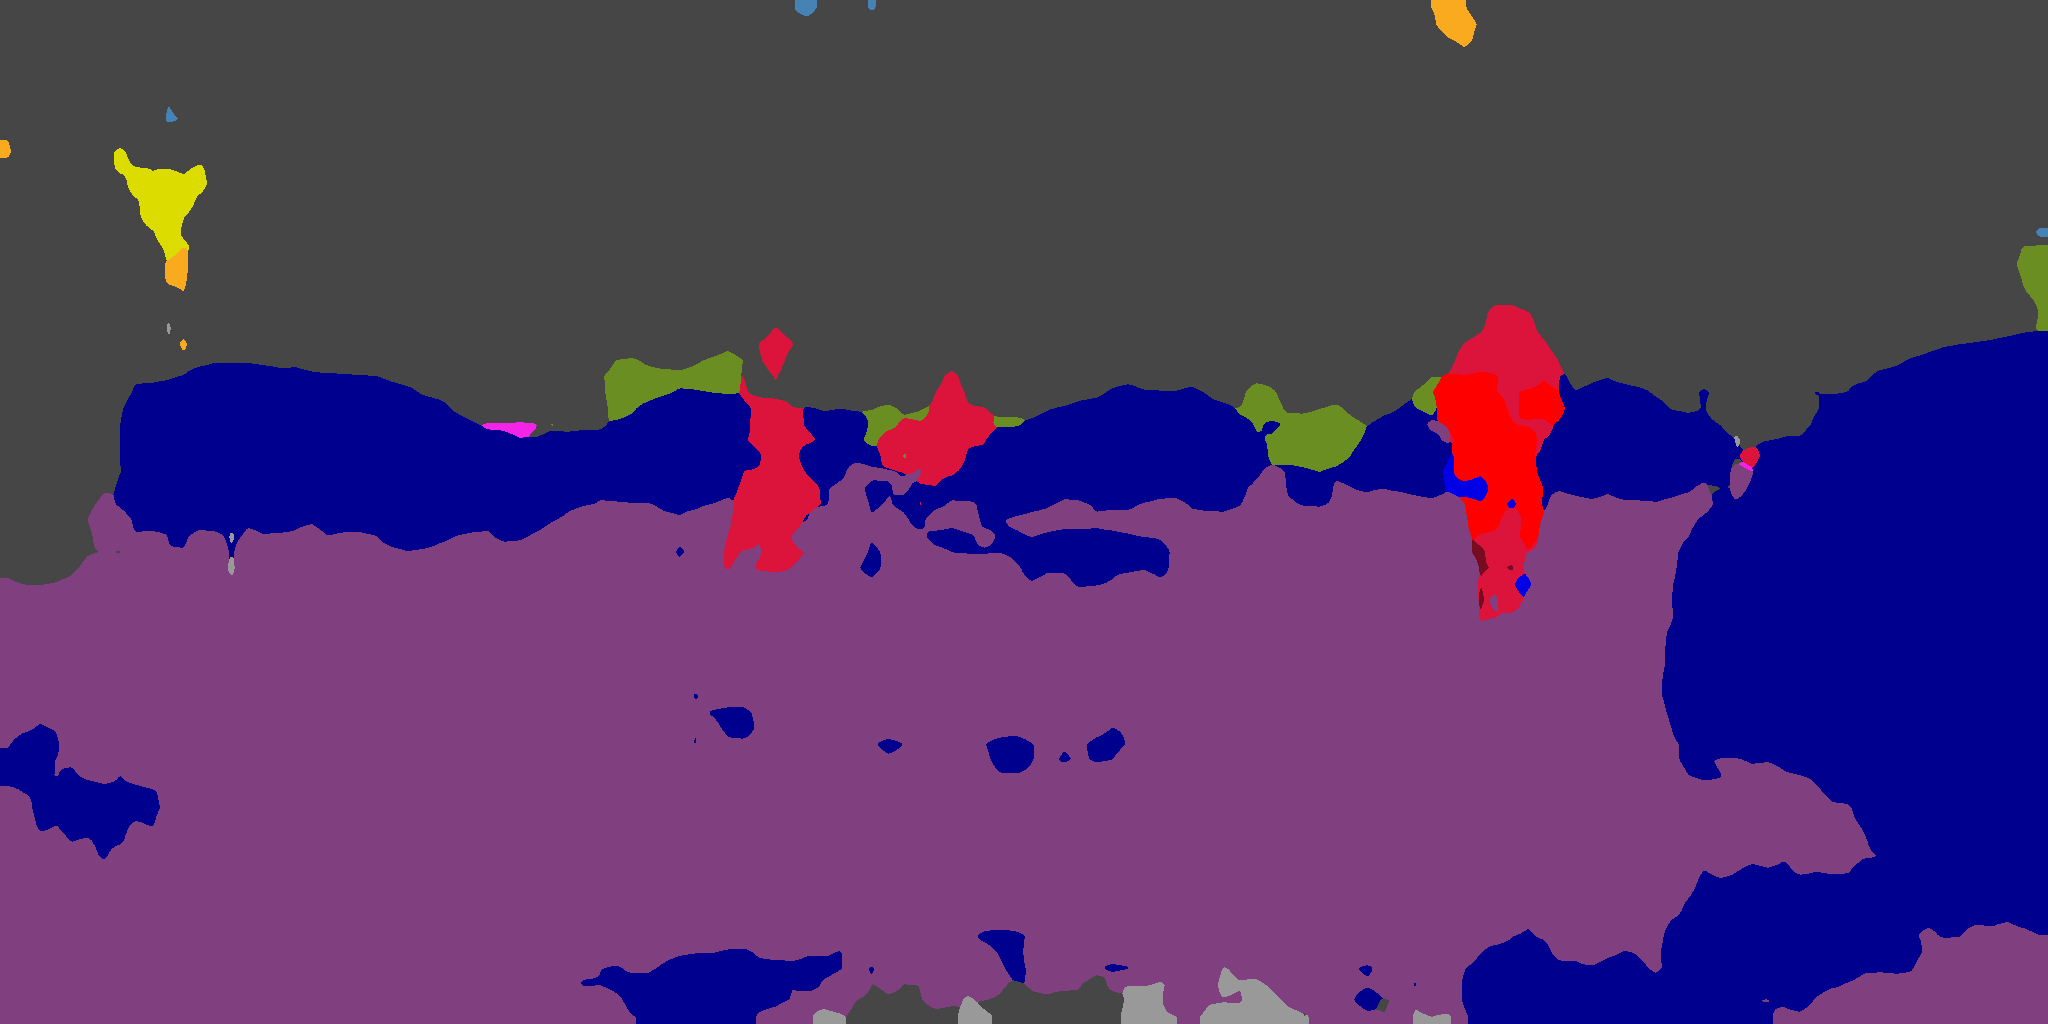
\includegraphics[width=.3\linewidth,valign=m]{res/lightweight-uda-baseline-qualitative/topformer-base-sourceonly.png}     & \includegraphics[width=.3\linewidth,valign=m]{res/lightweight-uda-baseline-qualitative/topformer-base-selftraining.png}     \\
        Topformer-Tiny     & \includegraphics[width=.3\linewidth,valign=m]{res/lightweight-uda-baseline-qualitative/topformer-tiny-sourceonly.png}     & \includegraphics[width=.3\linewidth,valign=m]{res/lightweight-uda-baseline-qualitative/topformer-tiny-selftraining.png}     \\
        MobileViT-Small    & \includegraphics[width=.3\linewidth,valign=m]{res/lightweight-uda-baseline-qualitative/mobilevit-small-sourceonly.png}    & \includegraphics[width=.3\linewidth,valign=m]{res/lightweight-uda-baseline-qualitative/mobilevit-small-selftraining.png}    \\
        MobileViT-XX-Small & \includegraphics[width=.3\linewidth,valign=m]{res/lightweight-uda-baseline-qualitative/mobilevit-xx-small-sourceonly.png} & \includegraphics[width=.3\linewidth,valign=m]{res/lightweight-uda-baseline-qualitative/mobilevit-xx-small-selftraining.png} \\
        Fast-SCNN          & \includegraphics[width=.3\linewidth,valign=m]{res/lightweight-uda-baseline-qualitative/fast-scnn-sourceonly.png}          & N/A                                                                                                                         \\
        SegFormer-B0       & \includegraphics[width=.3\linewidth,valign=m]{res/lightweight-uda-baseline-qualitative/segformer-mitb0-sourceonly.png}    & \includegraphics[width=.3\linewidth,valign=m]{res/lightweight-uda-baseline-qualitative/segformer-mitb0-selftraining.png}    \\
        DAFormer-B0        & \includegraphics[width=.3\linewidth,valign=m]{res/lightweight-uda-baseline-qualitative/daformer-mitb0-sourceonly.png}     & \includegraphics[width=.3\linewidth,valign=m]{res/lightweight-uda-baseline-qualitative/daformer-mitb0-selftraining.png}     \\
    \end{tabular}
    % }
    \caption{Qualitative baseline experiment results.}
    \label{fig: lightweight-model-baseline}
\end{figure}

\subsection{Applying UDA methods}
We subsequently attempt to apply the state-of-the-art DAFormer self-training strategies to the provided models.

Fast-SCNN was also found to significantly degrade in performance during self-training, which may be as it is unable to produce effective pseudo-labels early in training which only serve to further reduce it's accuracy. Therefore, we did not complete this experiment with Fast-SCNN.

As may be expected, SegFormer and DAFormer, the models around which the DAFormer training pipeline was designed, significantly outperform the competition. All models see improvement from the application of self-training, though to a much lesser extent than SegFormer and DAFormer. Therefore, we find applying domain adaptation most effectively to efficient architectures requires a different approach.

\subsection{FLOPs and parameter measurement}

FLOPs and parameters were measured using a script from the official SegFormer repository. The nuances of the script and our implementations of the models relative to the originals make the results somewhat unreliable, however, and most suitable for comparing the relative computing cost of different versions of the same model (e.g. MobileViT-Small vs MobileViT-XX-Small) due to the similar model layouts. For instance, TopFormer-Tiny appears to have significantly less parameters than its TopFormer-Base counterpart. Therefore, both iterations of TopFormer appear to be the strongest-performing segmentation models for the segmentation task.

\section{Pseudo-Teacher UDA}
After assessing the baseline transferability of small transformer-based segmentation methods, we move to our primary contribution - the creation of an effective UDA approach for lightweight segmentation networks. Our final approach is based on two key intuitions: First, it is unlikely that significantly smaller neural networks, even transformers, can mirror the effectiveness of their larger counterparts - they simply do not possess as much capacity to represent transferable features. Secondly, from a practical standpoint, large improvements in inference time/efficiency are often more valuable than large reductions in training time. Therefore, we propose the following: If smaller and more efficient models struggle with domain adaptation, why don't we simply delegate the task of learning transferable representations to a larger model? This "teacher" model can then be used to provide its target distribution information to the small, "student" model.

\begin{figure}[ht]
    \centering
    \includegraphics[width=\textwidth]{res/pseudo-teacher-pipeline.pdf}
    \caption{The pseudo-teacher pipeline.}
    \label{fig:pseudo-teacher-pipeline}
\end{figure}

Our Pseudo-Teacher method follows this approach by having the student learn from the teacher's most obvious and flexible representations of the target distribution - its target dataset pseudo-labels. In essence, we first train a large UDA segmentation model (in our case the state-of-the-art DAFormer \cite{hoyer_daformer_2022}) to learn the target distribution, then use it to produce pseudo-labels on the entire target dataset. These pseudo-labels are then used to train a much smaller segmentation model to make accurate predictions on the target set, without it having to perform any UDA itself.

Many existing approaches are similar to our pseudo-teacher UDA. Knowledge distillation involves using the soft outputs of a larger model to train a smaller one, with the soft outputs allowing the small model to learn how to represent features. An industry approach sometimes known as autolabelling involves using a pre-trained neural network to predict on many unlabelled samples, then manually adjusting these samples to quickly produce large datasets. However, our approach does not use soft labels for simplicity, and is targeted specifically at teaching domain-adapted features.

\subsection{Experimental Results}
As TopFormer was the best efficient network for source-only training (and our pseudo-teacher UDA does not involve other means of UDA), we opted to use it for our experiments. As with other UDA tasks, we do not allow our model, including the teacher model, to see validation set images during training. For our pseudo-teacher, we use DAFormer-B5 with the same experimental settings as outlined in the DAFormer paper \cite{hoyer_daformer_2022}.

\begin{table}[h]
    \resizebox{\textwidth}{!}{%
        \begin{tabular}{|l|l|r|r|r|r|}
            \hline
            Model             & UDA Approach       & \multicolumn{1}{l|}{Source-Only} & \multicolumn{1}{l|}{With UDA} & \multicolumn{1}{l|}{Oracle} & \multicolumn{1}{l|}{\begin{tabular}[c]{@{}l@{}}Relative \\ Performance\end{tabular}} \\ \hline
            TopFormer-Base    & Pseudo-Teacher & \textbf{33.32}                   & \textbf{61.18}                & 66.56                       & 91.92\%                                                                              \\ \hline
            TopFormer-Tiny    & Pseudo-Teacher & 27.78                            & 56.26                         & 59.39                       & \textbf{94.73\%}                                                                     \\ \hline
            DAFormer (MiT-B0) & Self-Training  & 28.12                            & 47.55                         & \textbf{70.78}              & 67.18\%                                                                              \\ \hline
        \end{tabular}
    }
    \caption{Results of Pseudo-Teacher UDA on GTA \textrightarrow CS. All performance values are in \% mIoU}
\end{table}

TopFormer's pseudo-teacher results are extremely impressive. With only ImageNet pre-training, TopFormer is able to achieve 61.18\% mean IoU using the teacher labels, an almost 40\% improvement over performing direct self-training with the most lightweight DAFormer. It achieves all this while still possessing significantly fewer parameters (figure \autoref{tab:lightweit-da-baseline}). TopFormer-Tiny also sees an incredible jump in performance, and both models achieve results near 90\% of those we observe when the training set is made available. This indicates that, even though the DAFormer-B5 teacher only achieves 68.3\% mIoU on the dataset itself, the smaller models are able to accurately learn the most relevant information to achieve similar results. In the qualitative results, the efficient model's ability to mirror fine details like signs and traffic lights is significantly of note, something efficient models previously struggled with in UDA..

\begin{table}[hb]
    \resizebox{\textwidth}{!}{%
        \begin{tabular}{lllll}
            \centering
            Ground Truth   &                   & \includegraphics[width=.2\linewidth,valign=m]{res/pseudo-teacher-qualitative/image.png}                     & \includegraphics[width=.2\linewidth,valign=m]{res/pseudo-teacher-qualitative/ground-truth.png}                  &                                                                                                         \\
            \textbf{Model} & \textbf{Approach} & \textbf{Source-Only}                                                                                        & \textbf{UDA}                                                                                                    & \textbf{Oracle}                                                                                         \\
            Topformer-Base & Pseudo-Teacher    & \includegraphics[width=.2\linewidth,valign=m]{res/pseudo-teacher-qualitative/topformer-base-sourceonly.png} & \includegraphics[width=.2\linewidth,valign=m]{res/pseudo-teacher-qualitative/topformer-base-pseudo-teacher.png} & \includegraphics[width=.2\linewidth,valign=m]{res/pseudo-teacher-qualitative/topformer-base-oracle.png} \\
            Topformer-Tiny & Pseudo-Teacher    & \includegraphics[width=.2\linewidth,valign=m]{res/pseudo-teacher-qualitative/topformer-tiny-sourceonly.png} & \includegraphics[width=.2\linewidth,valign=m]{res/pseudo-teacher-qualitative/topformer-tiny-pseudo-teacher.png} & \includegraphics[width=.2\linewidth,valign=m]{res/pseudo-teacher-qualitative/topformer-tiny-oracle.png} \\
            DAFormer       & Pseudo-Teacher    & \includegraphics[width=.2\linewidth,valign=m]{res/pseudo-teacher-qualitative/daformer-sourceonly.png}       & \includegraphics[width=.2\linewidth,valign=m]{res/pseudo-teacher-qualitative/daformer-uda.png}                  & \includegraphics[width=.2\linewidth,valign=m]{res/pseudo-teacher-qualitative/daformer-oracle.png}       \\
        \end{tabular}
    }
    \caption{Qualitative results of Pseudo-Teacher approach on Cityscapes dataset.}
    \label{fig:pseudo-teacher-qualitative}
\end{table}

Pre-training on the GTA dataset significantly reduced performance, the opposite of what was expected. This may be as the model is in a more generalisable state with only an ImageNet pre-trained backbone.

It is worth noting that the actual "oracle" accuracies of TopFormer are likely higher, but reduced due to nuances in our training approach, such as the use of $512 \times 512$ patches. TopFormer-base, for instance, reportedly achieves 75.0\% mIoU when trained at full resolution \cite{zhang_topformer_2022}.


\section{Conclusions}
We believe the under-explored domain of domain adaptation for efficient semantic segmentation has significant potential. Even in the simple approach we demonstrate here, we achieve extremely strong results. That training a small model on a domain-adaptive model's outputs would yield good results may not itself be surprising, but the extent of the performance increase is. Performance with TopFormer, for instance, is almost comparable to that of training with the target labels.
While this approach does not improve training-time speed, we do not consider a one-time training cost equivalent to approximately ~16 GPU hours with a single RTX 2080Ti prohibitively costly.

\section{Future work}
\begin{itemize}
    \item \textbf{Further datasets} - As in the previous chapter, further datasets should be explored for more comprehensive results.
    \item \textbf{Distillation} - The current approach simply trains the student model on the pseudo-teacher's output. Subsequent approaches could further communicate representation information by applying distillation techniques.
    \item \textbf{Application of domain adaptation techniques} - Domain adaptation techniques are used extensively in the teacher, but not the student. Taking advantage of target labels or applying domain regularisation techniques may further improve performance
    \item \textbf{Improving training time} - While the inference model is lightweight, training cost is limited by training of the teacher model. It may be beneficial to investigate memory usage specifically, as this will likely be a bottleneck for any application contexts where resources are limited.
\end{itemize}

\FloatBarrier

% \begin{figure}
%     \centering
%     \includegraphics[width=\textwidth]{}
%     \caption{example figure}
%     \label{fig:example-fig}
% \end{figure}

\chapter{Conclusion}
Semantic segmentation may be a fundamental task for computer vision, but its application in real-world scenarios requires extensive consideration. Through the development of SC-CrackSeg, we demonstrate it is possible to improve an application-level problem within semantic segmentation through the careful consideration of architecture. We also demonstrate that the ever-growing expressive potential of segmentation models makes certain approaches more challenging than before. While domain adversarial training had seen success in segmentation in the past, the dynamic adaptivity of transformer encoders combined with the nuanced feature space left us unable to make any improvement over baseline approaches. However, we find many specific application-level techniques remain unexplored. Through the application of our simple yet extremely effective pseudo-teacher approach, we allow lightweight segmentation models to achieve UDA performance that approaches results when target labels are available.

% \section{acknowledgement}
% Supervisors - Aneesh & Sonny

% ******************
\bibliography{thesis}{}
\bibliographystyle{IEEEtran}

\end{document}